\documentclass[twoside,12pt]{report}
\usepackage[polish]{babel}
\usepackage[T1]{fontenc}
\usepackage[utf8]{inputenc}
\usepackage{txfonts} % czcionka
\usepackage{graphicx}
\usepackage{pdfpages} % insert external PDF
\usepackage[unicode]{hyperref} % url
\usepackage{listings} % lstlisting
\usepackage{fancyhdr} % header and footer
\usepackage{indentfirst} % first paragraph ident
\usepackage{blindtext} % lorem impsum
\usepackage{geometry}
\usepackage{caption}
\usepackage{tabularx}

\widowpenalty=10000
\clubpenalty=10000
\brokenpenalty 10000 
\sloppy

\geometry{a4paper,left=35mm,right=25mm,top=25mm,bottom=25mm}

\renewcommand{\headrulewidth}{0.1pt}
\renewcommand{\chaptername}{Rozdział}
\renewcommand{\contentsname}{Spis treści}
\renewcommand{\figurename}{Rys.}
\renewcommand{\tablename}{Tab.}
\renewcommand{\lstlistingname}{Listing}
\renewcommand{\listfigurename}{Spis rysunków}
\renewcommand{\listtablename}{Spis tabel}
\renewcommand{\lstlistlistingname}{Spis listingów}
\renewcommand{\bibname}{Bibliografia}

\linespread{1.3} % Jeśli chcesz używać interlinii równej 1,5 jako wartość należy wstawić "1.3".

\pagestyle{fancy}
\fancyhf{}
\fancyhead[LE,RO]{\rightmark}
\fancyfoot[LE,RO]{\thepage}
\setlength{\headheight}{15.13202pt}
\setlength{\parindent}{1.5em}
\setlength{\emergencystretch}{3em}
\urlstyle{rm}

\let\oldsection\chapter
\def\chapter{\cleardoublepage\oldsection}

\newtheorem{definition}{Definicja} % przykład nowego środowiska 
\newtheorem{example}{Przykład}[chapter] % przykład nowego środowiska 
\newtheorem{corollary}{Wniosek}[chapter] % przykład nowego środowiska 

\begin{document}


\includepdf[pages={1,2}]{titlepage.pdf}

\tableofcontents	% generuje spis treści ze stronami

\chapter{Wstęp.} \label{rozdz.wstep} 

W rozdziale \ref{rozdz.wstep} zostały pokrótce opisane motywy wyboru tematu pracy dyplomowej i omówiono najważniejsze aspekty tej dziedziny. Ponadto w rozdziale umieszczono sformułowane cele pracy.

\section{Problematyka i~zakres pracy.}

Niniejsza praca obejmuje zagadnienia z~zakresu inżynierii oprogramowania i~sztucznej inteligencji. Głównym jej celem jest stworzenie aplikacji optymalizującej strukturę sieci drogowej.

Problemy komunikacji w~dzisiejszych miastach są wszystkim znane. Zatory drogowe i~korki w~godzinach szczytu są chlebem powszednim. Pomimo wielu prób i~sposobów, wciąż nie istnieje metoda jednoznacznie rozwiązująca tę kwestię. Bezspornie, dotyczy to wszystkich miast na świecie. Z~teoretycznego punktu widzenia, jedynym rozwiązaniem jest komunikacja publiczna. Oczywistym jest jednak, że nigdy nie doprowadzimy do sytuacji, gdy wszyscy mieszkańcy zrezygnują ze swoich pojazdów. Dodatkowo, wiele osób i~usług wymaga oddzielnej formy transportu. W~obliczu tych faktów miasta decydują się na rozwój swojej infrastruktury drogowej. Budowa nowych tras oraz poszerzanie starych przynosi nadzieję mniejszych zatorów, a~co za tym idzie, szybszego przejazdu do celu. Niestety, historia pokazuje, że takie inwestycje nie zawsze przynoszą oczekiwane korzyści.

Teorii próbujących wytłumaczyć te zjawiska, jak również dowodów, które je popierają lub obalają jest wiele. Jedną z~najpopularniejszych oraz taką która została wykorzystana w~niektórych miastach na świecie jest paradoks Braessa~\cite{braess}. Jest to twierdzenie matematyczne orzekające, że w~pewnym modelu ruchu drogowego, czasy podróży pojazdów mogą ulec wydłużeniu po dodaniu do sieci drogowej nowego połączenia. Ma ono również  zastosowanie w~przypadku  sieci komputerowych oraz istnieją jego analogie dla doświadczeń fizycznych.

Celem pracy jest opracowanie metody, która dla danej struktury sieci drogowej, zmodyfikuje ją wykorzystując prawidłowość z~powyższego paradoksu. W~efekcie poprzez zamknięcie wybranych ulic w~danej sieci drogowej, średni czas podróży powinien ulec skróceniu.

\section{Metoda badawcza i~cel pracy.}
\subsubsection{Studia literaturowe.}
Badania rozpoczęliśmy od poszukiwania źródeł traktujących o~opisywanym problemie. Paradoks Braessa został sformułowany w~1970 roku i~był od tego czasu wykorzystywany przy planowaniu przestrzeni i~infrastruktury wielu miast, np:

\begin{itemize}
\item Korea, Seul, likwidacja m.in. estakad Cheonggyecheon,
\item Niemcy, Stuttgart, likwidacja dróg zbudowanych w~latach 60,
\item USA, Nowy Jork, czasowe zamknięcie ulicy 42,
\item USA, Winnipeg.~\cite{urban}
\end{itemize}  

\subsubsection{Propozycja rozwiązania problemu.}
Oczywistym rozwiązaniem problemu komunikacji mogłoby być stworzenie idealnej sieci odpowiadającej potrzebom danego miasta. Rozbudowa lub modyfikacja tej infrastruktury jest jednak kosztowna i~czasochłonna. Z~tego powodu postanowiliśmy sprawdzić rozwiązanie zaproponowane przez Braessa. Ponieważ istnieją prace negujące lub podważające paradoks~\cite{newinsights} , zdecydowaliśmy by przy potwierdzaniu wyniku optymalizacji nie kierować się wyłącznie założeniami zawartymi w~twierdzeniu.

\subsubsection{Opis zastosowania algorytmów genetycznych.}
Ponieważ nie znaleźliśmy żadnych przesłanek wykazujących jednoznaczną ocenę co do słuszności zamknięcia danej ulicy, zdecydowaliśmy się na losowe przeszukiwanie przestrzeni rozwiązań.~Jednym z~rozwiązań w~przypadku takich poszukiwań są algorytmy genetyczne, które zostały wykorzystane w~pracy.

\subsubsection{Przedstawienie oceny optymalizacji.}
Paradoks Braessa zakłada dość oczywiste potwierdzenie swojej wiarygodności. Dlatego, w~celu potwierdzenia jego słuszności, zdecydowaliśmy się na zastosowanie zewnętrznego systemu oceny. Taką rolę spełniają systemy symulacji. System, który został wybrany działa zupełnie oddzielnie od metody twierdzenia, symulując rzeczywisty ruch na danej sieci drogowej. Wynik symulacji jest jednoznaczną wartością liczbową, przedstawiającą średni czas przejazdów wszystkich agentów biorących udział w~danym scenariuszu. Zakładając stały zestaw agentów dla zmieniających się w~wyżej opisany sposób sieci, dążymy oczywiście do minimalizacji średniego czasu przejazdu.

\subsubsection{Ocena możliwości wdrożenia proponowanych rozwiązań.}
Paradoks Braessa nie jest jedynym twierdzeniem traktującym o~problemach komunikacyjnych miast. Wiele teorii jest opartych głownie na socjologicznych lub psychologicznych założeniach\footnote{np. paradoks Downsa Thomsona~\cite{downs} czy prawo Lewisa Mogridge’a~\cite{lewis}}. Są jednak niemniej ważne. Biorąc pod uwagę złożoność problemu, wynik otrzymany podczas eksperymentu nie może być dowodem, ani decydującym głosem w~decyzjach dotyczących ustalaniu rzeczywistej sieci drogowej miasta. 


\section{Przegląd literatury w~dziedzinie.}
By przybliżyć temat problemów komunikacyjnych i~rozwiązania zaproponowanego przez Braessa polecamy pracę magisterską \textit{Leslie Arthura Keith Bloy}~\cite{investigation}. W~pracy zostały opisane również inne twierdzenia dotyczące ruchu drogowego. Publikacja \textit{Reducing the Effects of the Braess Paradox with Information Manipulation}~\cite{reducingtheeffects} jest bardzo dobrym uzupełnieniem tematu o~interesującą nas kwestię symulacji wieloagentowych. Prezentuje ona różnice w~wynikach dla przypadku losowego wyboru drogi przez agentów oraz tej wybranej przy użyciu inteligencji kolektywnej\footnote{ang. Collective Intelligence (COIN)}. 

Zbiorowa praca napisana na potrzeby międzynarodowej konferencji dotyczącej technologii symulacji~\cite{reducingtheeffects} jest pozycją, która opisuje podobny do podejmowanego przez nas problem. Mianowicie skupia się na modyfikacjach drogi poprzez zmiany dostępności jej składowych.

W zupełnie oddzielnej tematyce, algorytmów genetycznych, polecamy pozycję, która jest wstępem do tej tematyki~\cite{gene}. Pozycja zawiera bogaty zestaw problemów przykładowych wraz z~opisem ich rozwiązania. Ponadto dogłębnie opisuje ona każdy aspekt działania zastosowanych algorytmów. 

\section{Cel pracy.}
Tematem pracy jest optymalizacja struktury sieci drogowej. Za główny cel przyjęto stworzenie rozwiązania, które przy pomocy algorytmów genetycznych dokona optymalizacji sieci wejściowej. Optymalizacja zostanie przeprowadzona wykorzystując pewne ustalone z~góry parametry algorytmu genetycznego.
 
\section{Układ pracy.}
Rozdział \ref{rozdz.wstep} zawiera wstęp i~cele pracy. W~rozdziale \ref{rozdz.optymalizacja} przybliżamy istotę optymalizacji struktur sieci drogowych
oraz opisujemy teoretycznie, wykorzystane przeze nas rozwiązania. W~rozdziale \ref{rozdz.technologie} wymieniamy technologie, w~których wykonaliśmy aplikację oraz przybliżamy zewnętrzne biblioteki, o~które oparliśmy swoje rozwiązanie. Głównym rozdziałem pracy jest rozdział \ref{rozdz.opis},
w którym przedstawiamy wykonaną aplikację oraz wyniki optymalizacji przykładowej sieci. W~rozdziale podsumowującym \ref{rozdz.podsumowanie}, zawarliśmy wnioski oraz możliwości rozwoju pracy. Po rozdziale 5, podsumowującym, załączamy spis rysunków, tabel, listingów i~bibliografie, w~tej kolejności.

\chapter{Optymalizacja struktury sieci drogowej.}\label{rozdz.optymalizacja} 

W rozdziale \ref{rozdz.optymalizacja} zostały opisane teoretyczne aspekty pracy. Ich źródła opierają się o wybraną literaturę naukową.

\section{Podstawowe definicje.}

\begin{definition}\label{Graf nieskierowany}
\textbf{Grafem (nieskierowanym)} nazywamy parę zbiorów $(V,E)$. Elementy zbioru $V$ nazywają się \textit{wierzchołkami}, natomiast elementy zbioru $E$ nazywają się \textit{krawędziami}. Każda krawędź jest parą wierzchołków, tzn. $E \subseteq {{u,v}:u,v \in V}$~\cite{grafy}.
\end{definition}

\begin{figure}[ht]
\begin{center}
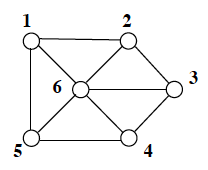
\includegraphics[width=0.40\textwidth]{img/graf1}
\caption{Przykładowy graf nieskierowany.} 
\end{center}
\end{figure}

Przykładowy graf nieskierowany może zostać opisany przez zbiory:
\begin{center}
\begin{math}
V=\{1,2,3,4,5,6\} \hspace*{40px} E=\{\{1,2\},\{2,3\},\{3,4\},\{4,5\},\{6,5\},\{6,1\},\{2,6\},\{3,6\},\{4,6\}\}
\end{math}
\end{center}

\vspace*{30px}
\begin{definition}\label{Graf skierowany}
\textbf{Grafem skierowanym} nazywamy taki graf, w~którym każda krawędź ma zdefiniowany początek i~koniec, tzn. żeby pary były uporządkowane. Wtedy $E \subseteq V \times V = {{u,v}:u,v \in V}$.
Krawędź $(u,v)$ najłatwiej wyobrazić sobie jako strzałkę od $u$ do $v$, dlatego często będziemy oznaczać ją przez $u \rightarrow v$~\cite{grafy}.
\end{definition}

\begin{figure}[ht]
\begin{center}
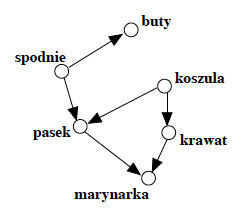
\includegraphics[width=0.40\textwidth]{img/graf2}
\caption{Przykładowy graf skierowany.} 
\end{center}
\end{figure}

Przykładowy graf skierowany może zostać opisany przez zbiory:
\newline
\begin{math}
V=\{spodnie, buty, pasek, koszula, krawat, marynarka\}
\end{math}
\newline
\begin{math}
E=\{\{spodnie \rightarrow buty\},\{spodnie  \rightarrow pasek\},
	\{pasek \rightarrow koszula\},\{koszula \rightarrow krawat\},
	\{pasek \rightarrow marynarka\},\{krawat \rightarrow marynarka\}\}
\end{math}

\section{Sieć drogowa w~postaci grafu}
W przypadku sieci drogowej mamy oczywiście do czynienia z~abstrakcyjną strukturą sieci. Przez sieć drogową rozumiemy bowiem układ dróg lub ulic np. w~mieście. Podczas swoich badań posługuję się zawsze pewnym fragmentem większej sieci. Najlepiej te dane zobrazuje poniższy przykład.

\begin{figure}[ht]
\begin{center}
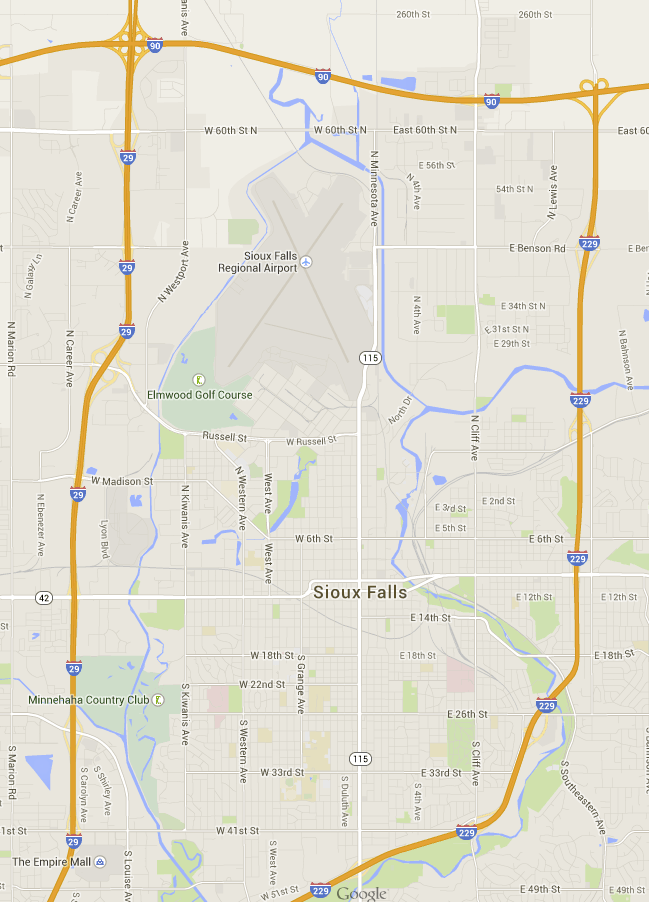
\includegraphics[width=0.35\textwidth]{img/siec}
\caption{Fragment sieci drogowej miasta Sioux Falls, Południowa Dakota.} 
\end{center}
\end{figure}

Posługując się powyższymi definicjami, tworząc graf z~pewnej sieci drogowej, przyjmujemy, że zbiorem $V$, wierzchołków są skrzyżowania, natomiast zbiór krawędzi $E$ odnosi się do ulic pomiędzy tymi skrzyżowaniami.
W pracy posługujemy się zawsze grafem skierowanym. W~związku z~tym, w~przypadku ulic dwukierunkowych tworzone są pary krawędzi z~odpowiednimi kierunkami, nawet jeśli ulice nie są rozłączne w~rzeczywistości.W celu potwierdzenia wiarygodności powyższego przykładu prezentujemy graf nałożony na mapę miasta~\cite{siux} na rysunkach \ref{left-ex}, \ref{right-ex}.

\vspace*{45px}
\begin{figure}[ht]
\begin{flushleft}
	\begin{minipage}[]{.45\textwidth}
	\centering
	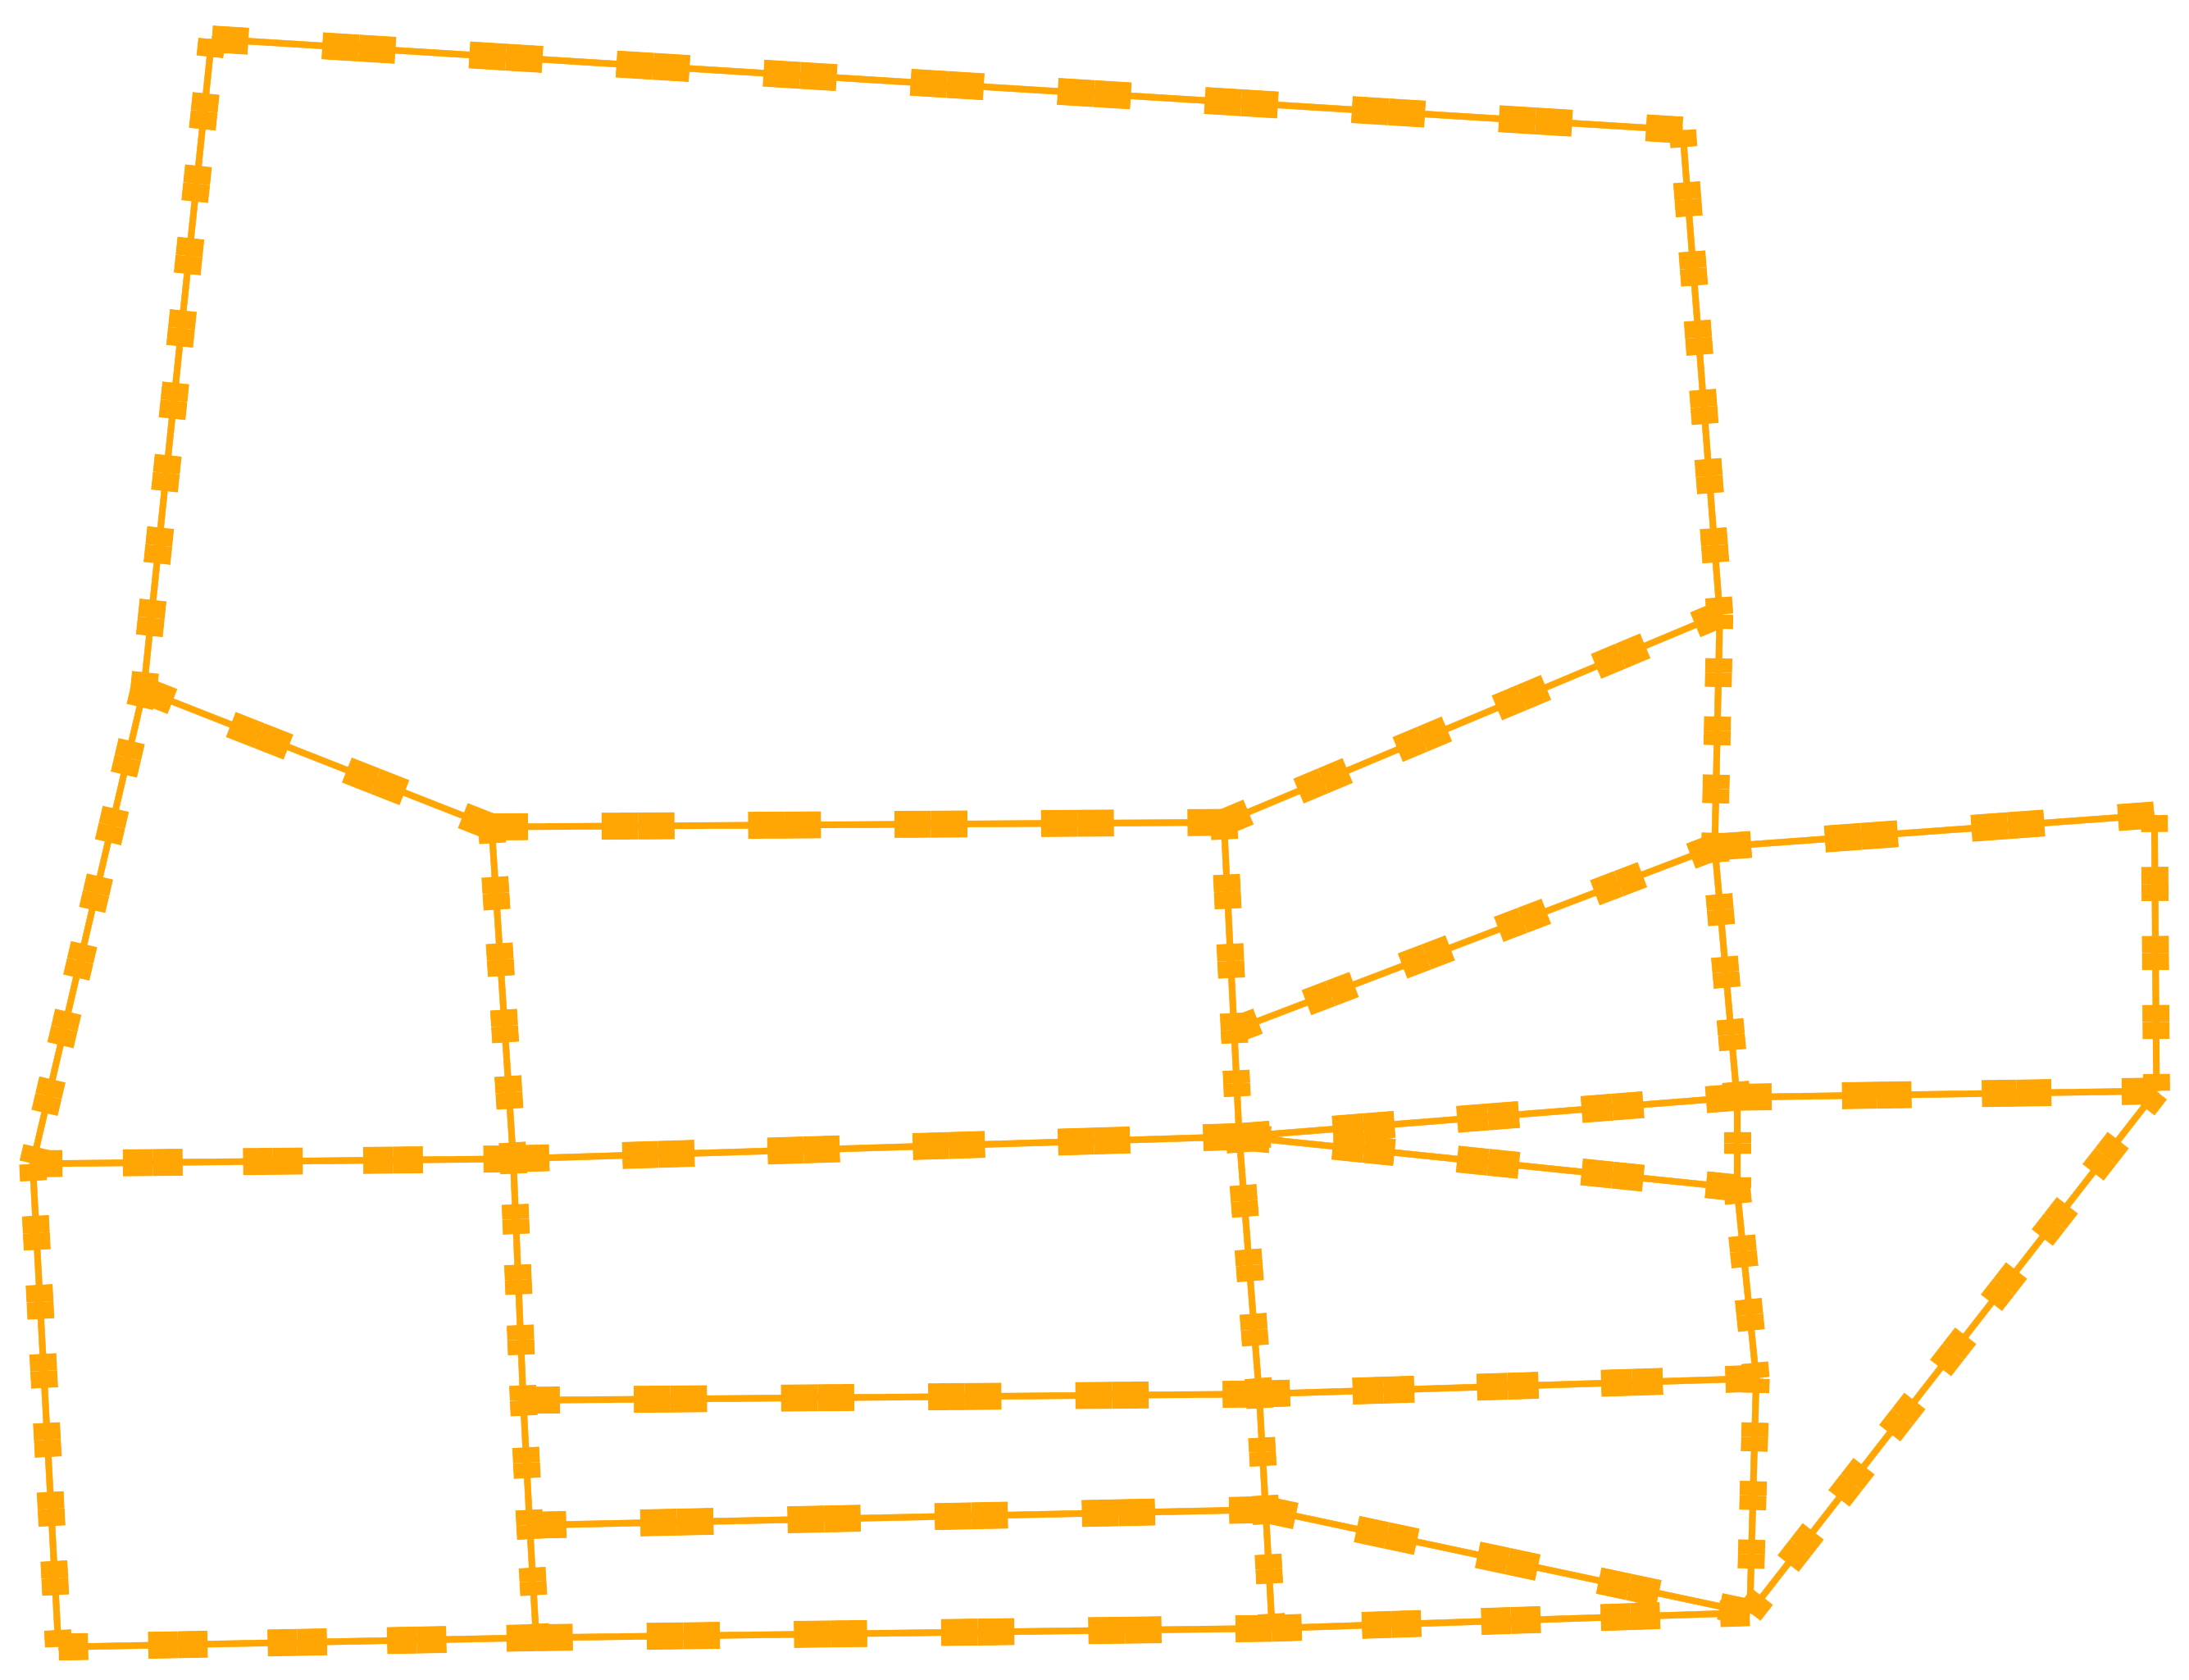
\includegraphics[width=\linewidth]{img/graf}
	\caption{Siec drogowa miasta Sioux Falls w postaci grafu.}
	\label{left-ex}
	\end{minipage}%
\end{flushleft}
\begin{flushright}
	\begin{minipage}[]{.45\textwidth}
	\centering
	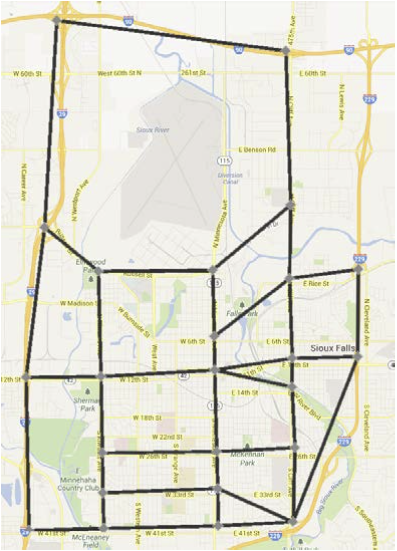
\includegraphics[width=\linewidth]{img/dopasowanie}
	\caption{Graf z dopasowaną geometrią.}
	\label{right-ex}
	\end{minipage}
\end{flushright}
\end{figure}

\clearpage
\section{Paradoks Braessa.}

Jak już wcześniej wspomnieliśmy, jest to twierdzenie matematyczne orzekające, że w~pewnym modelu ruchu drogowego czasy podróży pojazdów mogą ulec wydłużeniu po dodaniu do sieci drogowej nowego połączenia. Autorem twierdzenia jest niemiecki matematyk Dietrich Braess~\cite{braess}. Paradoks działa w~oparciu o~model ruchu drogowego, który ma następujące cechy:

\begin{enumerate}
\item Sieć drogowa składa się ze skończenie wielu węzłów i~łączących je odcinków dróg
\item Po sieci porusza się skończenie wiele pojazdów, każdy z~nich ma wyznaczony węzeł startowy i~węzeł docelowy
\item Odcinki dróg mają przypisane sobie czasy przejazdu, przy czym czasy te mogą zależeć od liczby pokonujących dany odcinek pojazdów.
\item Układ sieci drogowej i~czasy przejazdu poszczególnych odcinków są znane pojazdom
\item Celem pojazdów jest przejazd przez sieć z~węzłów początkowych do docelowych po trasie złożonej z~odcinków drogowych tak, by zminimalizować łączny czas ich pokonania
\item Decyzje o~wyborze tras pojazdy podejmują indywidualnie i~niezależnie od siebie
\end{enumerate}
Paradoks przedstawiamy w~oparciu o~przykład z~oryginalnego artykułu Dietricha Braessa~\cite{paradox}.

\subsection{Przykładowy, wyjściowy układ drogowy.}
\subsubsection{Sieć drogowa i~auta}

Przykład sytuacji, w~której ujawnia się paradoks Braessa jest skonstruowany z~czterech miast $A$, $B$, $X$ i~$Y$. Są one połączone odcinkami drogowymi jak na rysunku i~z~następującymi czasami przejazdu, przy czym $p$ oznacza gęstość ruchu w~tysiącach aut.


\begin{figure}[ht]
\vspace*{15px}
\begin{flushleft}
\begin{minipage}{.50\textwidth}
Autostrady:\newline
AX, $t_{AX}(p) =  50 + p$ min\newline
YB, $t_{YB}(p) =  50 + p$ min\newline

\vspace*{15px}
Drogi lokalne:\newline
AY, $t_{AY}(p) =  10p$ min\newline
XB, $t_{XB}(p) =  10p$ min\newline

\vspace*{15px}
Aut jest 6000 i wszystkie mają za zadanie przejechać trasę z $A$ do $B$.
\end{minipage}%
\end{flushleft}
\begin{flushright}
	\begin{minipage}{.50\textwidth}
	\centering
	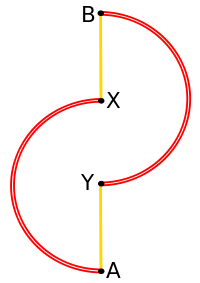
\includegraphics[width=0.7\textwidth]{img/braess1}
	\caption{Wyjściowy układ drogowy}
	\end{minipage}
\end{flushright}
\end{figure}


\subsubsection{Analiza równowagi Nasha}

Każde auto musi zdecydować się na wybór trasy albo $AXB$ albo $AYB$.

Równowaga Nasha to taka sytuacja, w~której każdy z~samochodów spowoduje wydłużenie swojego czasu jazdy, zmieniając decyzję co do wyboru trasy przy niezmienionych decyzjach pozostałych aut.
\newline\newline
Jeśli $p$ i~$q$ to liczby aut w~tysiącach pokonujących odpowiednio trasy $AXB$ i~$AYB$, otrzymujmy równania:

\begin{center}
\begin{math}
p+q = 6 \newline
t_{AX}(p)+t_{XB}(p) = t_{AY}(q) + t_{YB}(q) \newline
50+p+10p = 10q+50+q \newline
\end{math}
\end{center}
rozwiązaniem jest $p=q=3$.
Przy tej gęstości ruchu pokonanie obu dostępnych tras zabiera $50+3+30=83$ minuty.

\subsection{Przykładowy, uzupełniony układ drogowy.}
\subsubsection{Sieć drogowa i~auta}
Do wyjściowego układu drogowego dodana zostaje autostrada:

\begin{figure}[ht]
\vspace*{15px}
\begin{flushleft}
	\begin{minipage}{.50\textwidth}
	Autostrady:\newline
	YX, $t_{YX}(p) =  10 + p$ min\newline
	
	\vspace*{15px}
	Aut jest nadal 6000 i wszystkie mają za zadanie przejechać trasę z $A$ do $B$.
	\end{minipage}%
\end{flushleft}
\begin{flushright}
	\begin{minipage}{.50\textwidth}
	\centering
	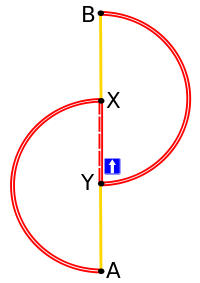
\includegraphics[width=0.7\textwidth]{img/braess2}
	\caption{Uzupełniony układ drogowy}
	\end{minipage}
\end{flushright}
\end{figure}

\subsubsection{Analiza równowagi Nasha}

Jeśli $p$, $q$ i~$r$ to liczby aut w~tysiącach pokonujących odpowiednio trasy $AXB$, $AYB$ i~$AYXB$, otrzymujmy równania:

\begin{center}
\begin{math}
p+q+r = 6 \newline
t_{AX}(p)+t_{XB}(p+r) = t_{AY}(q+r) + t_{YB}(q) = t_{AY}(q+r)+t_{YX}(r)+t_{XB}(p+r)\newline
50+p+10(p+r) = 10(q+r)+50+q = 10(q+r)+ 10 + r + 10(p+r)\newline
\end{math}
\end{center}
rozwiązaniem jest $p=q=r=2$.
Czas przejazdu każdej z~tych dróg wynosi wówczas $50+2+10(2+2)=92$ minuty.

\subsection{Wyjaśnienie intuicyjne.}
Wąskim gardłem systemu są drogi lokalne, na których czas przejazdu bardzo szybko wzrasta wraz z~intensywnością ruchu. Po pojawieniu się dodatkowej drogi dostępna staje się nowa trasa, prowadząca oprócz nowego skrótu YX tylko drogami lokalnymi.

Z perspektywy całości systemu nowy odcinek drogowy odciąża ruch na autostradach, gdzie jest to mało odczuwalne, a~w~zamian jeszcze bardziej zagęszcza ruch na drogach lokalnych, powodując wydłużenie czasu podróży.

\section{Graf skierowany silnie spójny.}
Na potrzeby symulatora, sieć drogowa przedstawiona w~postaci grafu skierowanego musi spełniać warunek silnej spójności. 
\newline
\begin{definition}\label{Graf silnie spójny}
\textbf{Grafem skierowanym silnie spójnym} nazywamy graf skierowany w~którym jest możliwe dotarcie do każdego wierzchołka zaczynając z~dowolnego innego poprzez dowolną ilość krawędzi. Wszystkie wierzchołki w~grafie skierowanym silnie spójnym muszą zatem posiadać przynajmniej jedną krawędź wchodzącą i~wychodzącą\cite{silniespojny}.
\end{definition}

W sprawdzaniu grafu pod względem spójności, wykorzystujemy algorytm Tarjana do znajdowania składowych silnie spójnych.
\newline
\begin{definition}\label{Algorytm Tarjana}
Podstawowym założeniem \textbf{algorytmu Tarjana} jest przeszukiwanie grafu w~głąb zaczynając od dowolnego wierzchołka wybranego w~sposób arbitralny. Tak jak w~przypadku klasycznego przeszukiwania w~głąb, każdy sąsiadujący wierzchołek po odwiedzeniu zostaje oznaczony i~algorytm nigdy ponownie go nie odwiedza. Dzięki temu, tworzymy kolekcję przeszukanych drzew, która jest drzewem rozpinającym grafu. Składowe silnie spójne są następnie odnajdowane jako poddrzewa, a~korzenie tych poddrzew są nazywane korzeniami składowych silnie spójnych. Każdy wierzchołek grafu może być wybrany na korzeń składowej silnie spójnej jeśli zostanie wybrany jako pierwszy wierzchołek podczas przeszukiwania w~głąb.
\end{definition}

\vspace*{15px}

\begin{definition}
\textbf{Składowa silnie spójna} (ang. strongly connected component) jest maksymalnym pod grafem, w~którym istnieją ścieżki pomiędzy każdymi dwoma wierzchołkami. Jeśli pod graf ten obejmuje wszystkie wierzchołki grafu, to mówimy, że dany graf skierowany jest silnie spójny (ang. strongly connected digraph). W~grafach nieskierowanych każdy graf spójny jest również silnie spójny.
\end{definition}

\begin{figure}[ht]
\centering
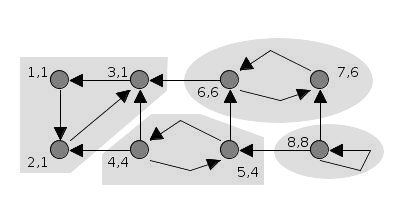
\includegraphics[width=0.6\textwidth]{img/tajran}
\caption{Przykładowy graf z zaznaczonymi składowymi silnie spójnymi.}
\end{figure}

W efekcie, zawsze przed rozpoczęciem symulacji sprawdzamy, czy graf jest grafem skierowanym silnie spójnym lub dokładniej mówiąc, czy posiada tylko jedną składową silnie spójną.

\section{Klasyczny algorytm genetyczny.}

Idea algorytmu genetycznego została zaczerpnięta z~nauk przyrodniczych opisujących zjawiska doboru naturalnego i~dziedziczenia. Mechanizmy te polegają na
przetrwaniu osobników najlepiej dostosowanych w~danym środowisku, podczas gdy
osobniki gorzej przystosowane sa eliminowane. Z~kolei te osobniki, które przetrwają
- przekazują informacje genetyczną swoim potomkom. Krzyżowanie informacji genetycznej otrzymanej od ,,rodziców'' prowadzi do sytuacji, w~której kolejne pokolenia sa przeciętnie coraz lepiej dostosowane do warunków środowiska; mamy tu więc do czynienia ze swoistym procesem optymalizacji. 

\subsection{Podstawowe pojecia algorytmów genetycznych}

\begin{definition}
\textbf{Populacją} nazywamy zbiór osobników o~określonej liczebności.
\end{definition}

\vspace*{10px}

\begin{definition}
\textbf{Osobnikami} populacji w~algorytmach genetycznych są zakodowane w~postaci chromosomów zbiory parametrów zadania, czyli rozwiązania, określone też jako punkty
przestrzeni poszukiwań.~Osobniki czasami nazywa się organizmami.
\end{definition}

\vspace*{10px}

\begin{definition}
\textbf{Chromosomy} to inaczej łańcuchy lub ciągi kodowe, to uporządkowane ciągi genów.
\end{definition}

\vspace*{10px}

\begin{definition}
\textbf{Gen} – nazywany też cechą, znakiem, detektorem – stanowi pojedynczy element
genotypu, w~szczególności chromosomu. Genotyp, czyli struktura, to zespół chromosomów
danego osobnika. Zatem osobnikami populacji mogą być genotypy albo
pojedyncze chromosomy.
\end{definition}

\vspace*{10px}

\begin{definition}
\textbf{Fenotyp} jest zestawem wartości odpowiadających danemu genotypowi, czyli zdekodowana
struktura, a~wiec zbiorem parametrów zadania (rozwiązaniem, punkt przestrzeni
poszukiwań).
\end{definition}

\vspace*{10px}

\begin{definition}
\textbf{Allel} to wartość danego genu, określona jako wartość cechy lub wariant cechy.
\end{definition}

\vspace*{10px}

\begin{definition}
\textbf{Locus} to pozycja - wskazuje miejsce położenia danego genu w~łańcuchu, czyli chromosomie.
\end{definition}

\vspace*{10px}

\begin{definition}
\textbf{Funkcja przystosowania nazywana tez funkcją dopasowania lub funkcja oceny.} Stanowi ona miarę przystosowania (dopasowania) danego osobnika w~populacji.
\end{definition}

\subsection{Algorytm klasycznego algorytmu genetycznego.}

Na podstawowy (klasyczny) algorytm genetyczny, nazywany także elementarnym
lub prostym algorytmem genetycznym, składają się kroki:

\begin{enumerate}
\item inicjacja czyli wybór początkowej populacji chromosomów,
\item ocena przystosowania chromosomów w~populacji,
\item sprawdzenie warunku zatrzymania,
\item selekcja chromosomów,
\item zastosowanie operatorów genetycznych,
\item utworzenie nowej populacji,
\item wyprowadzenie najlepszego chromosomu.
\end{enumerate}

Najłatwiej wyobrazić sobie powyższe kroki analizując je na schemacie:

\begin{figure}[ht]
\begin{center}
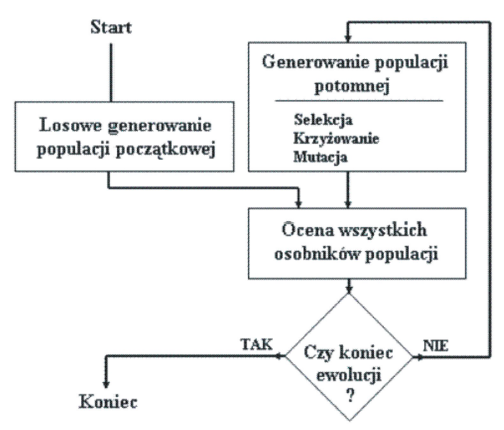
\includegraphics[width=0.6\textwidth]{img/ogolgene}
\caption{Ogólny schemat algorytmu genetycznego.}
\end{center}
\end{figure}

\subsection{Operacje klasyczne, krzyżowanie.}

Operacja krzyżowania jest podstawową operacją algorytmów genetycznych służącą do rekombinacji materiału genetycznego. Operacja opiera się na dwóch chromosomach, których części materiału genetycznego zostają wymieszane w~celu otworzenia nowego chromosomu. Podstawowa operacja krzyżowania opiera się o~jeden punkt krzyżowania i~została przedstawiona na poglądowym schemacie \ref{krzyzowanie}~\cite{gene mutikrzyz}.

\begin{figure}[ht]
\begin{center}
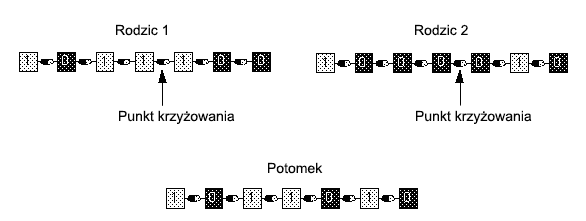
\includegraphics[width=\textwidth]{img/crossover}
\caption{Ogólny schemat operacji krzyżowania.}
\label{krzyzowanie}
\end{center}
\end{figure}

\subsection{Operacje klasyczne, mutacja.}

Proces rekombinacji przez krzyżowanie nie byłby w~stanie odkryć całej przestrzeni poszukiwań, jeżeli dana kombinacja nie byłaby obecna w~sekcjach populacji. To mogłoby prowadzić do błędnego wyniku. Operacja mutacji pozwala na wprowadzenie nowych struktur genetycznych w~obecnej populacji. Dokonuje tego poprzez losową zmianę dowolnego genu w~chromosomie~\cite{gene mutikrzyz}.

\begin{figure}[ht]
\begin{center}
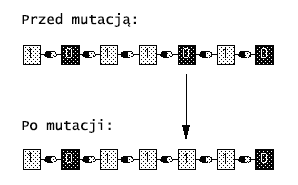
\includegraphics[width=0.580\textwidth]{img/mutation}
\caption{Ogólny schemat operacji mutacji.}
\end{center}
\end{figure}

\section{Użycie grafów w~algorytmie genetycznym.}

W swojej pracy posługuję się przede wszystkim grafami. W~tym wypadku klasyczna odmiana algorytmu genetycznego musiałaby zostać zmodyfikowana na potrzeby wykorzystania grafów jako chromosomów. Dodatkowo wymagałoby to zastosowania nowych sposobów krzyżowania i~mutacji jednostek. 

Zdecydowaliśmy, że zamiast przystosowywać algorytm genetyczny do nowej struktury, przystosujemy strukturę do algorytmu. Ponieważ naszym zadaniem jest zdecydowanie o~zamknięciu lub nie, danej ulicy (krawędzi grafu) postanowiłem opisać tę strukturę jako listę opisującą ten stan. Zgodnie z~tą myślą, sieć drogowa (graf) jest tłumaczona na tablicę elementów przyjmujących wartości:

\begin{itemize}
\item 1 (prawda) - dla ulicy (węzła), który jest przejezdny,
\item 0 (fałsz) - dla ulicy (węzła) zamkniętego dla ruchu.
\end{itemize}

Tablica tworzona w~ten sposób może być modyfikowana przez algorytm genetyczny, jak również bez problemu możemy z~niej odtworzyć stan obecny sieci drogowej. Za przykład podajemy sytuację przedstawioną na rysunkach \ref{left-example} i~\ref{right-example}.


\begin{figure}[ht]
\begin{flushleft}
	\begin{minipage}[c]{.47\textwidth}
	\vspace*{80px}
	\centering
	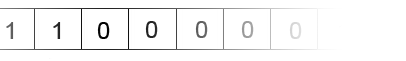
\includegraphics[width=\textwidth]{img/bool}
	\caption{Fragment sieci w postaci tablicy binarnej }
	\label{left-example}
	\end{minipage}%
\end{flushleft}
\begin{flushright}
	\begin{minipage}[c]{.47\textwidth}
	\centering
	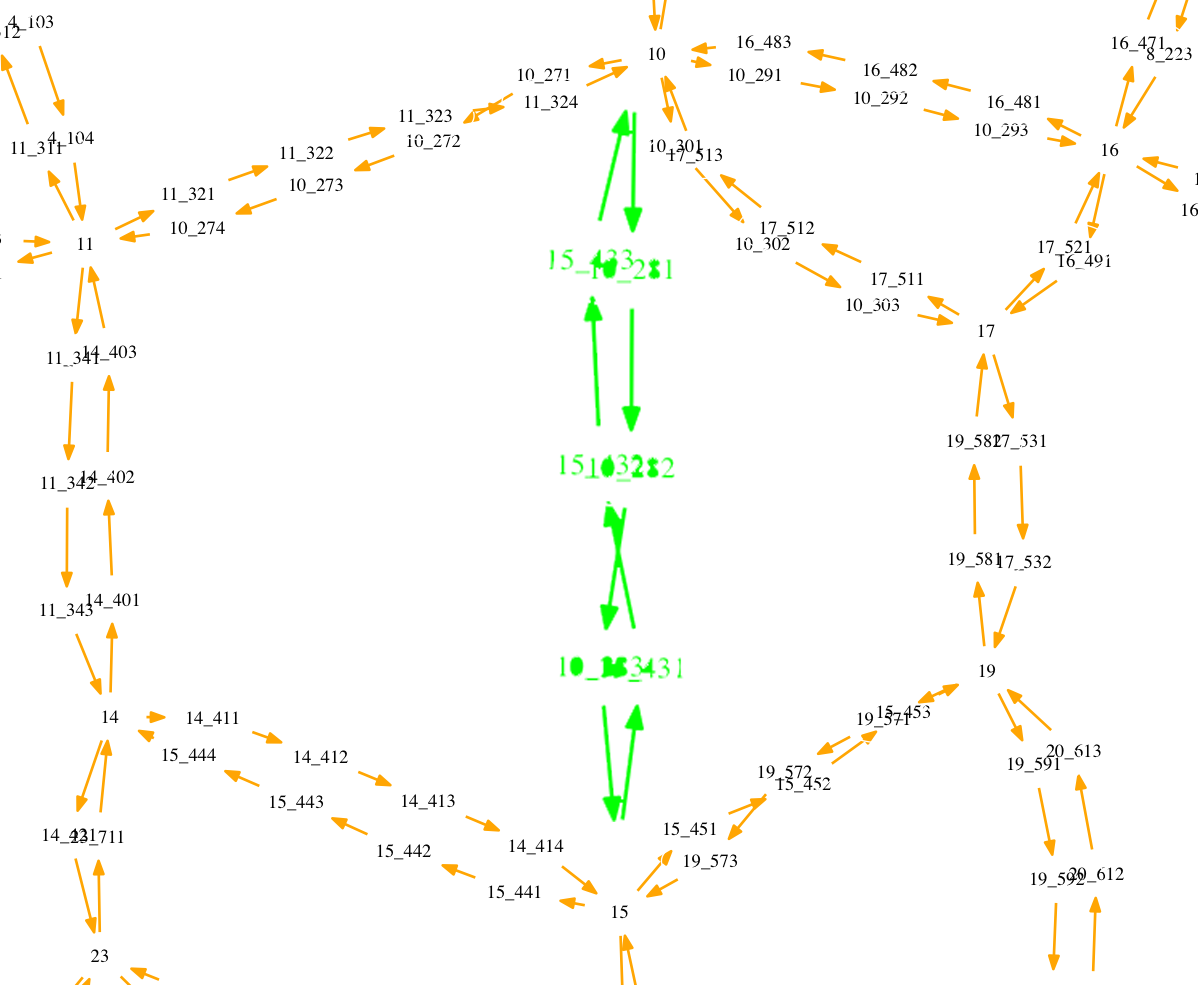
\includegraphics[width=\textwidth]{img/bool-efect}
	\caption{Fragment sieci w postaci grafu}
	\label{right-example}
	\end{minipage}
\end{flushright}
\end{figure}

Przedstawiony na rysunku \ref{left-example} fragment sieci zawiera kolejne elementy zerowe, które w~tłumaczeniu na przykładowy graf \ref{right-example}, są zaznaczone kolorem zielonym. W~tym przypadku krawędzie te zostaną wyłączone z~ruchu. 

\section{Punkty artykulacji grafu.}

Punktem artykulacji\footnote{ang. articulation point lub cut vertex} jest wierzchołek, którego usunięcie z~grafu spowoduje zwiększenie liczby spójnych składowych. Na rysunku \ref{artykulacja}, punktem artykulacji jest wierzchołek o~numerze $0$.

\begin{figure}[ht]
\begin{center}
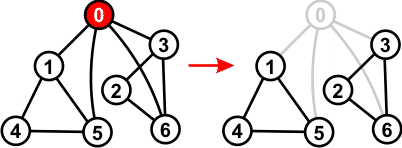
\includegraphics[width=0.7\textwidth]{img/articulation}
\caption{Przykład grafu z zaznaczonym punktem artykulacji.}
\label{artykulacja}
\end{center}
\end{figure}

Algorytm poszukiwania punktów artykulacji wykorzystuje przeszukiwanie grafu w~głąb. Podczas nierekurencyjnego przejścia, wierzchołek zostaje oznaczony jako punkt artykulacji, wtedy i~tylko wtedy, jeśli jest on korzeniem posiada więcej niż dwóch synów. A~wierzchołek $ v $ nie będący korzeniem drzewa DFS jest punktem artykulacji wtedy i~tylko wtedy, gdy przynajmniej dla jednego jego syna nie istnieje krawędź wtórna $ \{u,w\} $, taka że wierzchołek $ u~$ jest potomkiem $ v $ i~$ w~$ jest przodkiem $ v $.

Punkty te są wykorzystywane, by podczas losowych mutacji i~krzyżowań w~algorytmie genetycznym nie doszło do stworzenia grafu innego niż grafu skierowanego silnie spójnego. Krok sprawdzenia jest wykonywany podczas każdorazowego zamykania drogi, zatem za każdym razem gdy zostaje wprowadzona nowa wartość ,,$0$'' w~tablicy.

\chapter{Technologie i~metody użyte.}\label{rozdz.technologie} 

W rozdziale \ref{rozdz.technologie} zostają przedstawione technologie wykorzystane w projekcie, jak również krótki opis ich wykorzystania. Załączamy także opis systemu, na którym zostały wykonane obliczenia.

\section{Symulator transportu.}

MATSim jest środowiskiem\footnote{ang. framework, pl. szkielet do budowy aplikacji} do implementacji szerokiej skali symulacji transportu opartych na agentach. Składa się z~wielu modułów, które mogą zostać połączone lub używane oddzielnie. Moduły można zastępować własnymi implementacjami w~celu przetestowania pojedynczych aspektów pracy~\cite{matsim}.

\begin{figure}[ht]
\centering

\includegraphics[width=0.40\textwidth]{img/matsim}
\caption{Logo symulatora transportu MATSim} 
\end{figure}

Oczywiście MATSim nie jest jedynym dostępnym symulatorem transportu. Podobnych rozwiązań jest wiele. Wybór motywowaliśmy jednak przede wszystkim dostępnością materiałów szkoleniowych i~przykładowymi scenariuszami. MATSim jest żywym projektem oparty o~licencję open source\footnote{pol. otwarte oprogramowanie}. Dysponuje szerokim zasobem przykładów i~gotowych scenariuszy, w~dodatku udostępniając prace wielu osób na swoim repozytorium.

\section{Algorytmy genetyczne.}

Projekt The Apache Commons jest tworzony przez Apache Software Foundation. Głównym celem projektu jest stworzenie wolnego oprogramowania do wielokrotnego użytku w~języku Java. Projekt podzielony jest na trzy główne części: proper, sandbox, i~dormant~\cite{math}.

W przypadku głównej części Apache Commons Proper wyróżniamy wiele modułów różniących się funkcjonalnością i~celem. Apache Commons Math jest modułem zapewniającym rozwiązywania problemów głównie matematycznych i~statystycznych. Znajduje się w~nim implementacja podstawowej formy algorytmu genetycznego, którą rozszerzamy w~pracy.

\begin{figure}[ht]
\centering

\includegraphics[width=0.50\textwidth]{img/math}
\caption{Logo biblioteki Apache Commons Math} 
\end{figure}

\section{Obsługa grafów.}

Ponieważ moduł do wizualizacji rozwiązań MATSim nie spełniał naszych oczekiwań zarówno pod względem wydajności jak i~stabilności zdecydowaliśmy się na stworzenie własnej implementacji. W~tym celu wykorzystaliśmy dojrzały projekt NetworkX.~Jest to biblioteka wykonana w~języku Python stworzona z~myślą o~grafach i~sieciach. Jest ona dostarczana jako darmowe oprogramowanie na licencji BSD-new~\cite{networkx}. 

\begin{figure}[ht]
\centering
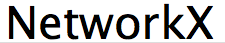
\includegraphics[width=0.40\textwidth]{img/networkx}
\caption{Logo biblioteki NetworkX} 
\end{figure}

\section{Technologie i~metodologie programistyczne.}

Użyte przez nas technologie są poniekąd wymuszone przez języki w~jakich zostały stworzone wykorzystywane pomocnicze rozwiązania. W~przypadku symulatora MATSim jest to Java. Zdecydowaliśmy się natomiast na wykorzystanie Pythona głównie ze względu na przeważającą przewagę biblioteki NetworkX nad bibliotekami obsługującymi grafy w~języku Java. Nie jest to wyjątek, gdyż ogólnie rozwiązania dostarczane dla Python'a, szczególnie w~przypadku problemów akademickich, są dużo lepsze. Poniżej zestaw narzędzi, które wykorzystaliśmy w~procesie tworzenia aplikacji.  

\begin{figure}[ht]
\begin{flushleft}
	\begin{minipage}[]{.47\textwidth}
	\centering
	
\includegraphics[width=0.8\textwidth]{img/java}
	\caption{Logo Java.}
\end{minipage}%
\end{flushleft}
\begin{flushright}
	\begin{minipage}[]{.47\textwidth}
	\centering
	
\includegraphics[width=0.8\textwidth]{img/eclipse}
	\caption{Logo IDE Eclipse.}	
	\end{minipage}
\end{flushright}
\end{figure}

\begin{figure}[ht]
\begin{flushleft}
	\begin{minipage}[]{.47\textwidth}
	\vspace*{30px}
	\centering
	
\includegraphics[width=0.8\textwidth]{img/py}
	\caption{Logo Python.}
	\end{minipage}%
\end{flushleft}
\begin{flushright}
	\begin{minipage}[]{.47\textwidth}
	\centering
	
\includegraphics[width=0.8\textwidth]{img/pydev}
	\caption{Logo PyDev.}
	\end{minipage}
\end{flushright}
\end{figure}

Logo pochodzą ze stron dostawców~\cite{java, eclipse, python,pydev}.

\section{Wdrożenie.}

Ze względu na duże wymagania sprzętowe obliczeń, a~zarazem ograniczoną przenośność rozwiązania z~powodu skorzystania z~Pythona, zdecydowaliśmy się na usprawnienie rozwiązania. Wykorzystując system Linux Ubuntu stworzyliśmy maszynę wirtualną spełniającą wszystkie wymagania do uruchomienia aplikacji. Dzięki temu stało się możliwe wykorzystanie innych komputerów oprócz tego, na którym zostało stworzone rozwiązanie. Pomijamy również dzięki temu problemy przystosowania czy instalowania dużej ilości zewnętrznego oprogramowania i~bibliotek~\cite{ubuntu}.

\begin{figure}[ht]
\centering

\includegraphics[width=0.4\textwidth]{img/ubuntu}
\caption{Logo systemu Linux Ubuntu.}
\end{figure}

W katalogach pracy znajduje się instrukcja wraz z~wymaganymi pakietami do uruchomienia projektu. Podczas badań wykorzystywany był system Linux Ubuntu~12.04~LTS.

\section{System obliczeniowy.}

Korzystając z~powyższego rozwiązania, dzięki któremu projekt jest możliwy do zainstalowania na innych maszynach, do obliczeń wykorzystaliśmy zewnętrznego dostawcę. Przy wyborze decydującym czynnikiem była cena rozwiązania, co w~przypadku chmury Microsoft Windows~\cite{azure}, pozwoliło na darmowe rozwiązanie\footnote{dzięki darmowemu okresowi próbnemu}.

\begin{figure}[ht]
\centering

\includegraphics[width=0.5\textwidth]{img/azure}
\caption{Logo chmury Microsoft Windows Azure.}
\end{figure}

\chapter{Opis projektu.}\label{rozdz.opis} 

W niniejszym rozdziale opisujemy strukturę projektu z~opisem jego uruchomienia. Ponieważ przeprowadzane przez projekt obliczenia wymagają wiele czasu, zdecydowaliśmy się na pominięcie interfejsu użytkownika przy projektowaniu aplikacji. Całość jest obsługiwana przez plik konfiguracyjny, który zostaje wczytany na początku operacji i~za jego pomocą kontrolujemy przebieg obliczeń.~Pomimo dwóch osobnych technologii, w~których został wykonany projekt, są one od siebie zależne. Całość jest obsługiwana przez projekt w~Java, skrypty w~Pythonie jedynie wspierają niektóre procesy.

\section{Dane wejściowe.}

Przykładowy plik konfiguracyjny dla projektu z~opisem jego funkcji przedstawiono na listingu \ref{exconfig}.

\lstset{
    language=xml,
    tabsize=3,
    rulesepcolor=\color{gray},
    keywordstyle=\color{blue}\bf,
    stringstyle=\color{red},
    breaklines=true,
    basicstyle=\ttfamily\scriptsize}
\lstinputlisting[language=Xml, caption=Plik konfiguracyjny projektu, label=exconfig]{img/config.xml} 

\vspace*{15px}

Jak widać konfiguracja dzieli się na trzy podstawowe grupy:
\begin{itemize}
\item project,
\item scenario,
\item genetics.
\end{itemize}

\vspace*{15px}

Grupa \textit{project} odpowiada za główne ustawienia całego projektu, w~\textit{scenario} znajdziemy ustawienia dotyczące symulacji przeprowadzanej przez MATSim, natomiast sekcja \textit{genetics} zawiera ustawienia dotyczące algorytmu genetycznego.

\vspace*{15px}

Wyjaśnienie opcji \textit{project}:
\begin{itemize}
\item name - nazwa projektu, używana jako katalog wyjściowy,
\item output dir - katalog, gdzie zapisujemy wyniki,
\item threads - ilość wątków, które mają być użyte podczas obliczeń,
\item log level - poziom logowania Log4J\footnote{zewnętrzna biblioteka do logowania, dostępne poziomy: DEBUG, INFO, WARN, ERROR i~FATAL},
\item python path - ścieżka instalacji Pythona,
\item python main - folder ze skryptami pomocniczymi,
\item java-path - ścieżka instalacji Javy,
\item matsim-jar - scieżka do biblioteki MATSim,
\item matsim-xmx - maksymalna pamięć RAM dostępna dla symulatora MATSim.
\end{itemize}

\vspace*{15px}

Wyjaśnienie opcji \textit{scenario}:
\begin{itemize}
\item config - scieżka dostępu pliku konfiguracyjnego scenariusz MATSim,
\item network - scieżka dostępu pliku z~siecią wejściową scenariusza,
\item population - scieżka dostępu pliku z~populacja scenariusza,
\item facilities - scieżka dostępu pliku z~budynkami scenariusza,
\item iterations - ilość iteracji symulacji MATSima.
\end{itemize}

\vspace*{15px}

Wyjaśnienie opcji \textit{genetics}:
\begin{itemize}
\item population size - rozmiar populacji,
\item max generations - ilość testowanych generacji (warunek stopu),
\item elitism rate - ilość najlepszych chromosomów biorących udział w~kolejnej iteracji,
\item crossover rate - szansa na krzyżowanie osobników,
\item mutation rate - szansa na mutacje osobników,
\item tournament rate - ilość osobników biorących udział w~turnieju.
\end{itemize}


\section{Badane miasto przykładowe: Sioux Falls}

Główną zaletą korzystania z~MATSima, o~której już wcześniej wspominaliśmy, jest dość pokaźny zbiór danych przykładowych. Jednym z~nich jest materiał zaprezentowany przez twórców aplikacji, który udostępnili w~2013 roku na zgromadzeniu użytkowników platformy~\cite{siux}. Przykład ten dotyczy miasta Sioux Falls w~Południowej Dakocie. Domyślnie scenariusz składa się z:

\begin{itemize}
\item dwóch grup zapotrzebowania bez charakterystyk socjodemograficznych:
\begin{itemize}
\item 68094 agentów z~samochodem oraz korzystających z~transportu publicznego,
\item 40877 agentów posiadających samochód.
\end{itemize}
\item dostosowanej sieci drogowa miasta Sioux Falls,
\item transportu publicznego razem z~rozkładem jazdy,
\item przykładowych miejsc zamieszkania, pracy i~rozrywki.
\end{itemize}

\vspace*{20px}
Po zapoznaniu się z~przykładem, dostarcza on nawet za dużo danych, które by nas interesowały. Dostosowaliśmy go zatem do swoich potrzeb poprzez:

\begin{itemize}
\item usunięcie transportu publicznego,
\item wyposażenie każdego agenta w~swój samochód.
\end{itemize}

Powyższe modyfikacje znacznie wzmogły ruch w~mieście (co było dla nas pozytywnym efektem) i~skróciły obliczenia związane z~symulacjami. Na rysunku \ref{siouxsiec} przedstawiamy sieć miasta odwzorowaną w~postaci grafu. Natomiast na rysunku \ref{siouxbudynki}  prezentujemy  rozkład miejsc pracy, domostw i~innych zakładów nałożonych na graf sieci drogowej miasta.

\begin{figure}[ht]
\centering
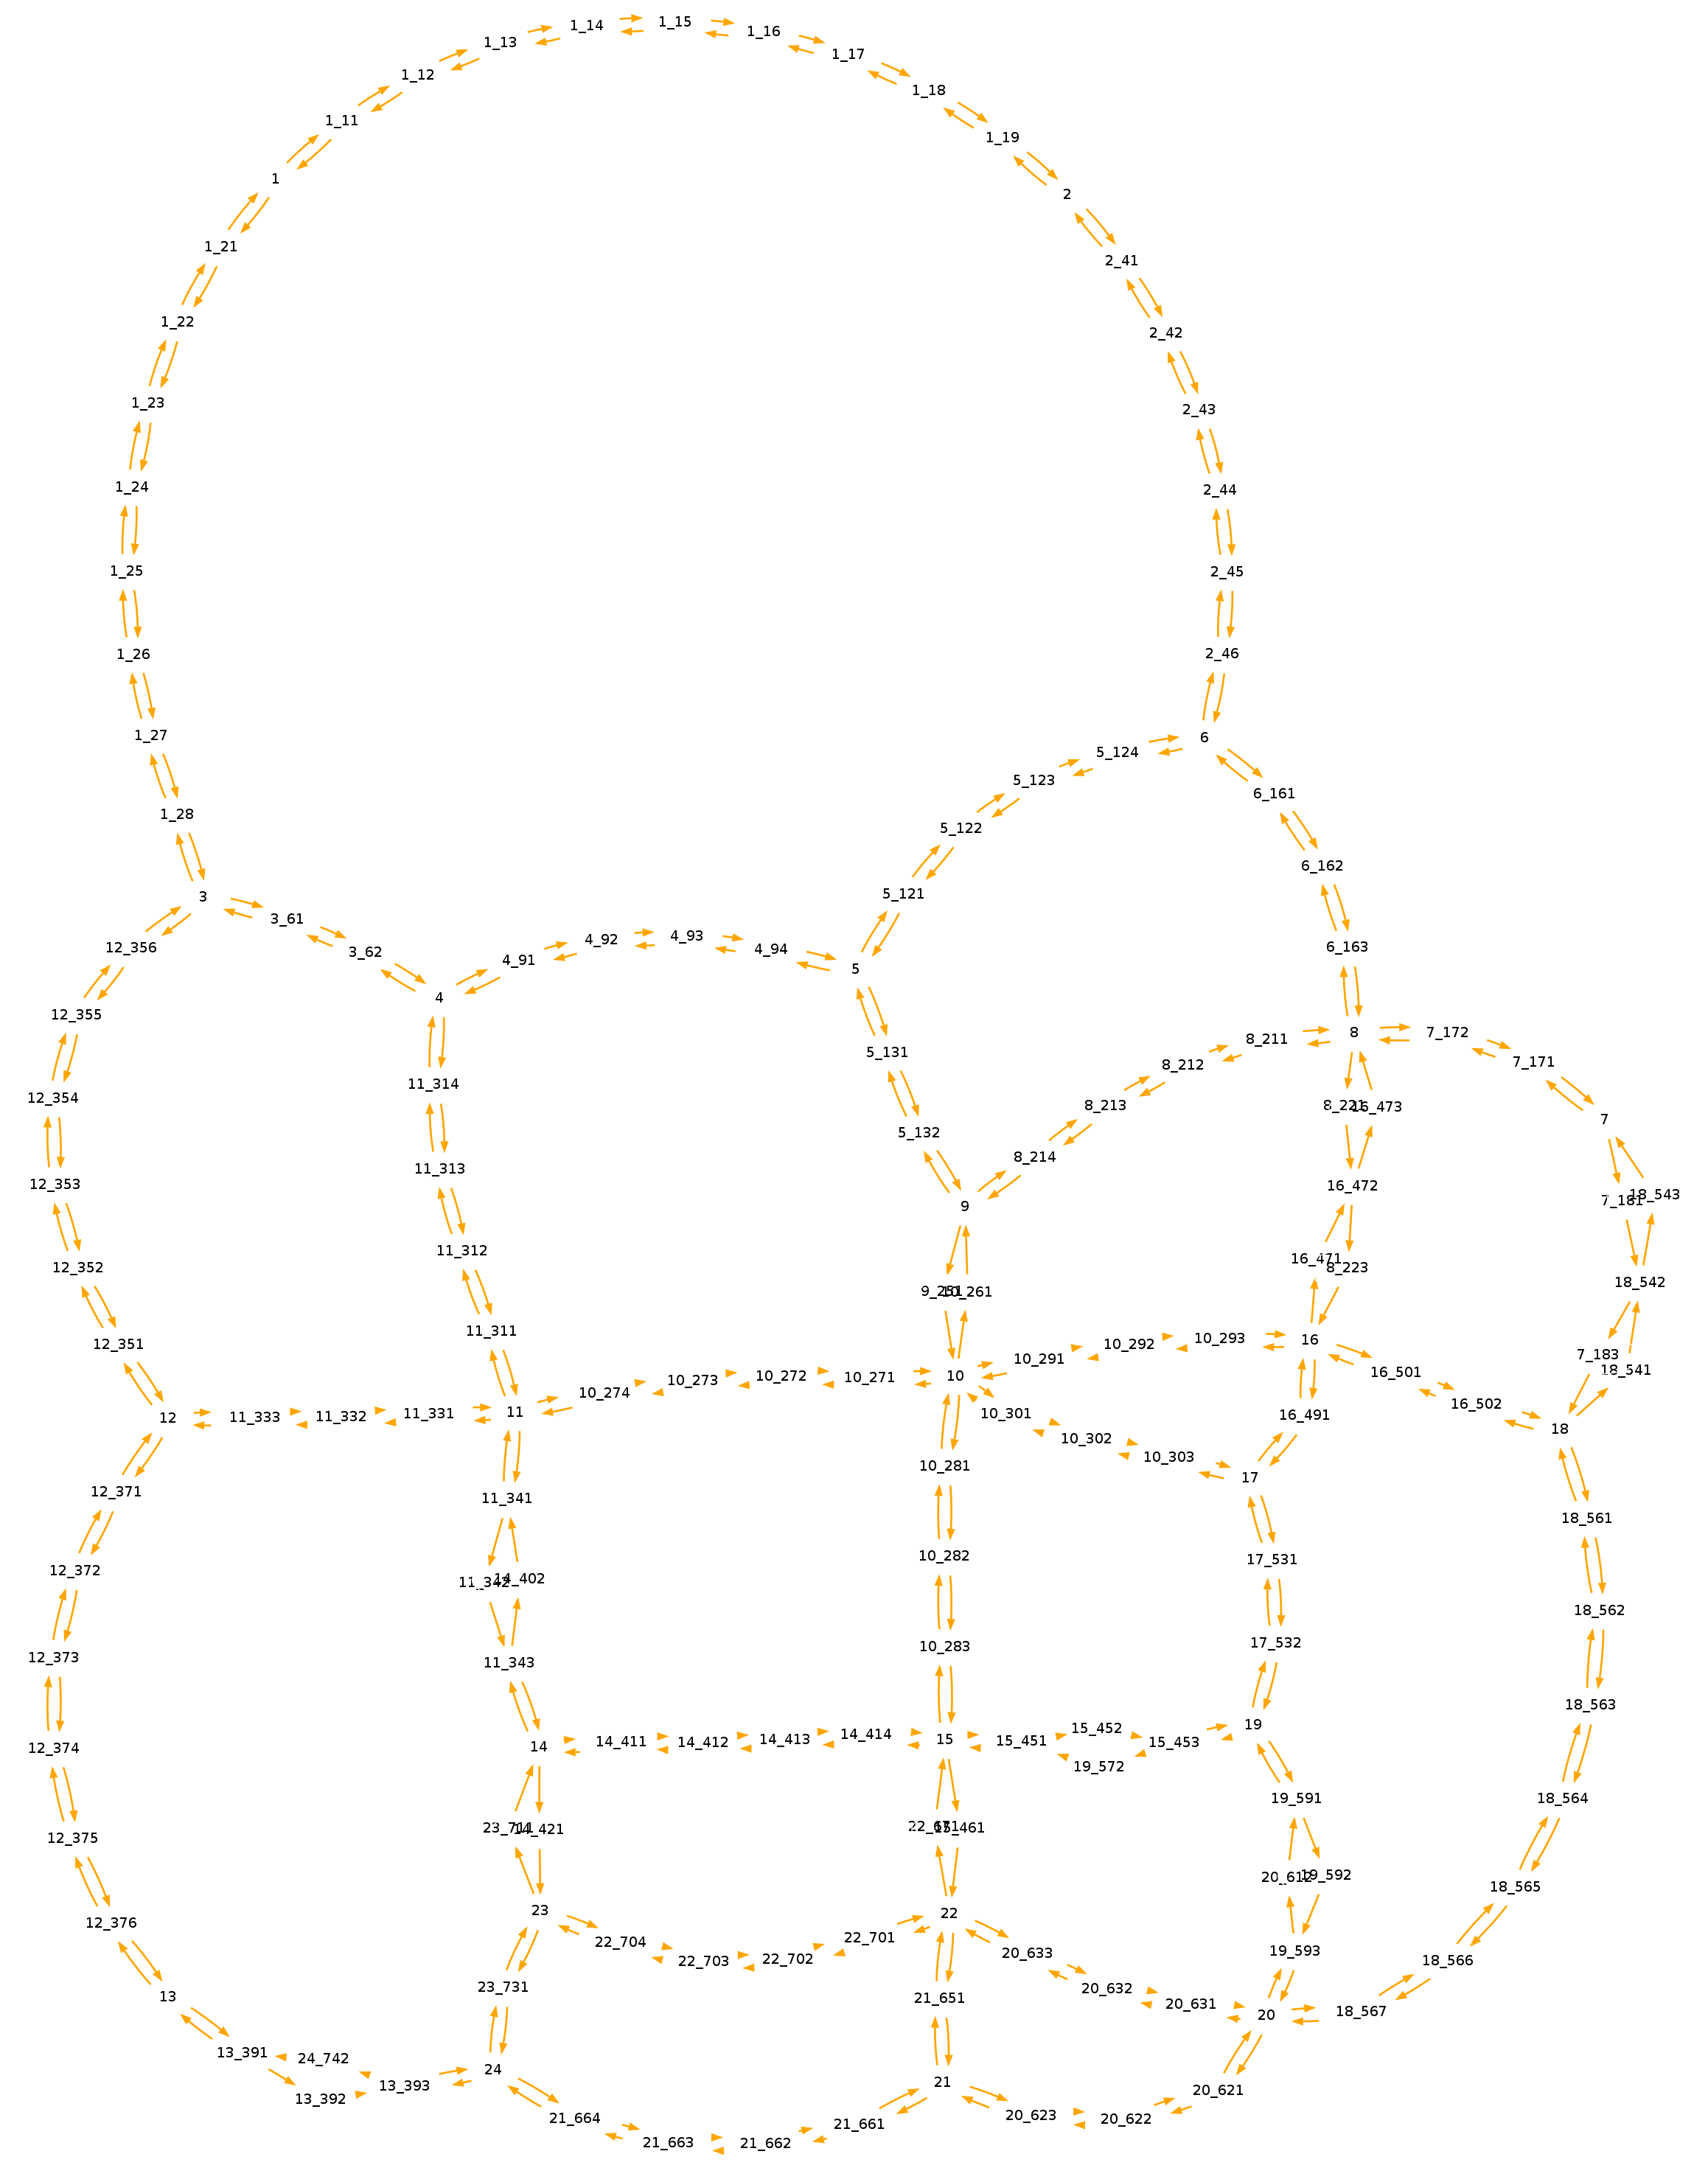
\includegraphics[totalheight=0.580\textheight]{img/sioux/network}
\caption{Graf sieci miasta Sioux Falls wykorzystany w badaniach.} 
\label{siouxsiec}
\end{figure}

\begin{figure}[ht]
\centering
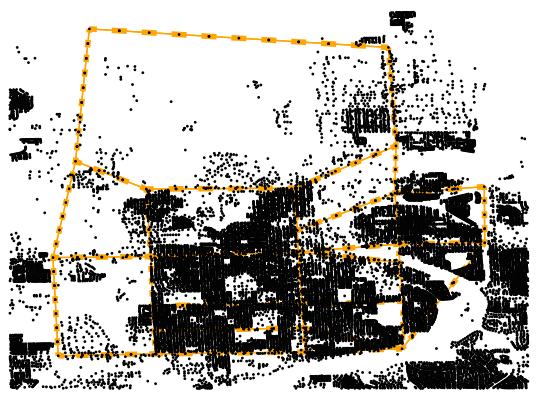
\includegraphics[width=1.2\textwidth]{img/sioux/facilities}
\caption{Rozkład budynków na grafie miasta Sioux Falls.} 
\label{siouxbudynki}
\end{figure}

Na rysunkach \ref{ex-sioux-1} i~\ref{ex-sioux-3} prezentujemy ruch drogowy w~najbardziej intensywnych godzinach dnia, tj. godzinach szczytu. Ruch jest przedstawiony jako natężenie ruchu na każdej krawędzi (ulicy), poprzez odniesienie go do możliwości przepustowości każdego węzła. Kolor zielony oznacza małe obciążenie, żółty średnie i~czerwony - wysokie natężenie ruchu w~tym miejscu. Rysunki są obrócone o~$90^{\circ}$ w~lewo, dla zwiększenia ich czytelności i~rozmiaru. 

\begin{figure}[ht]
\centering
%bottom right top left
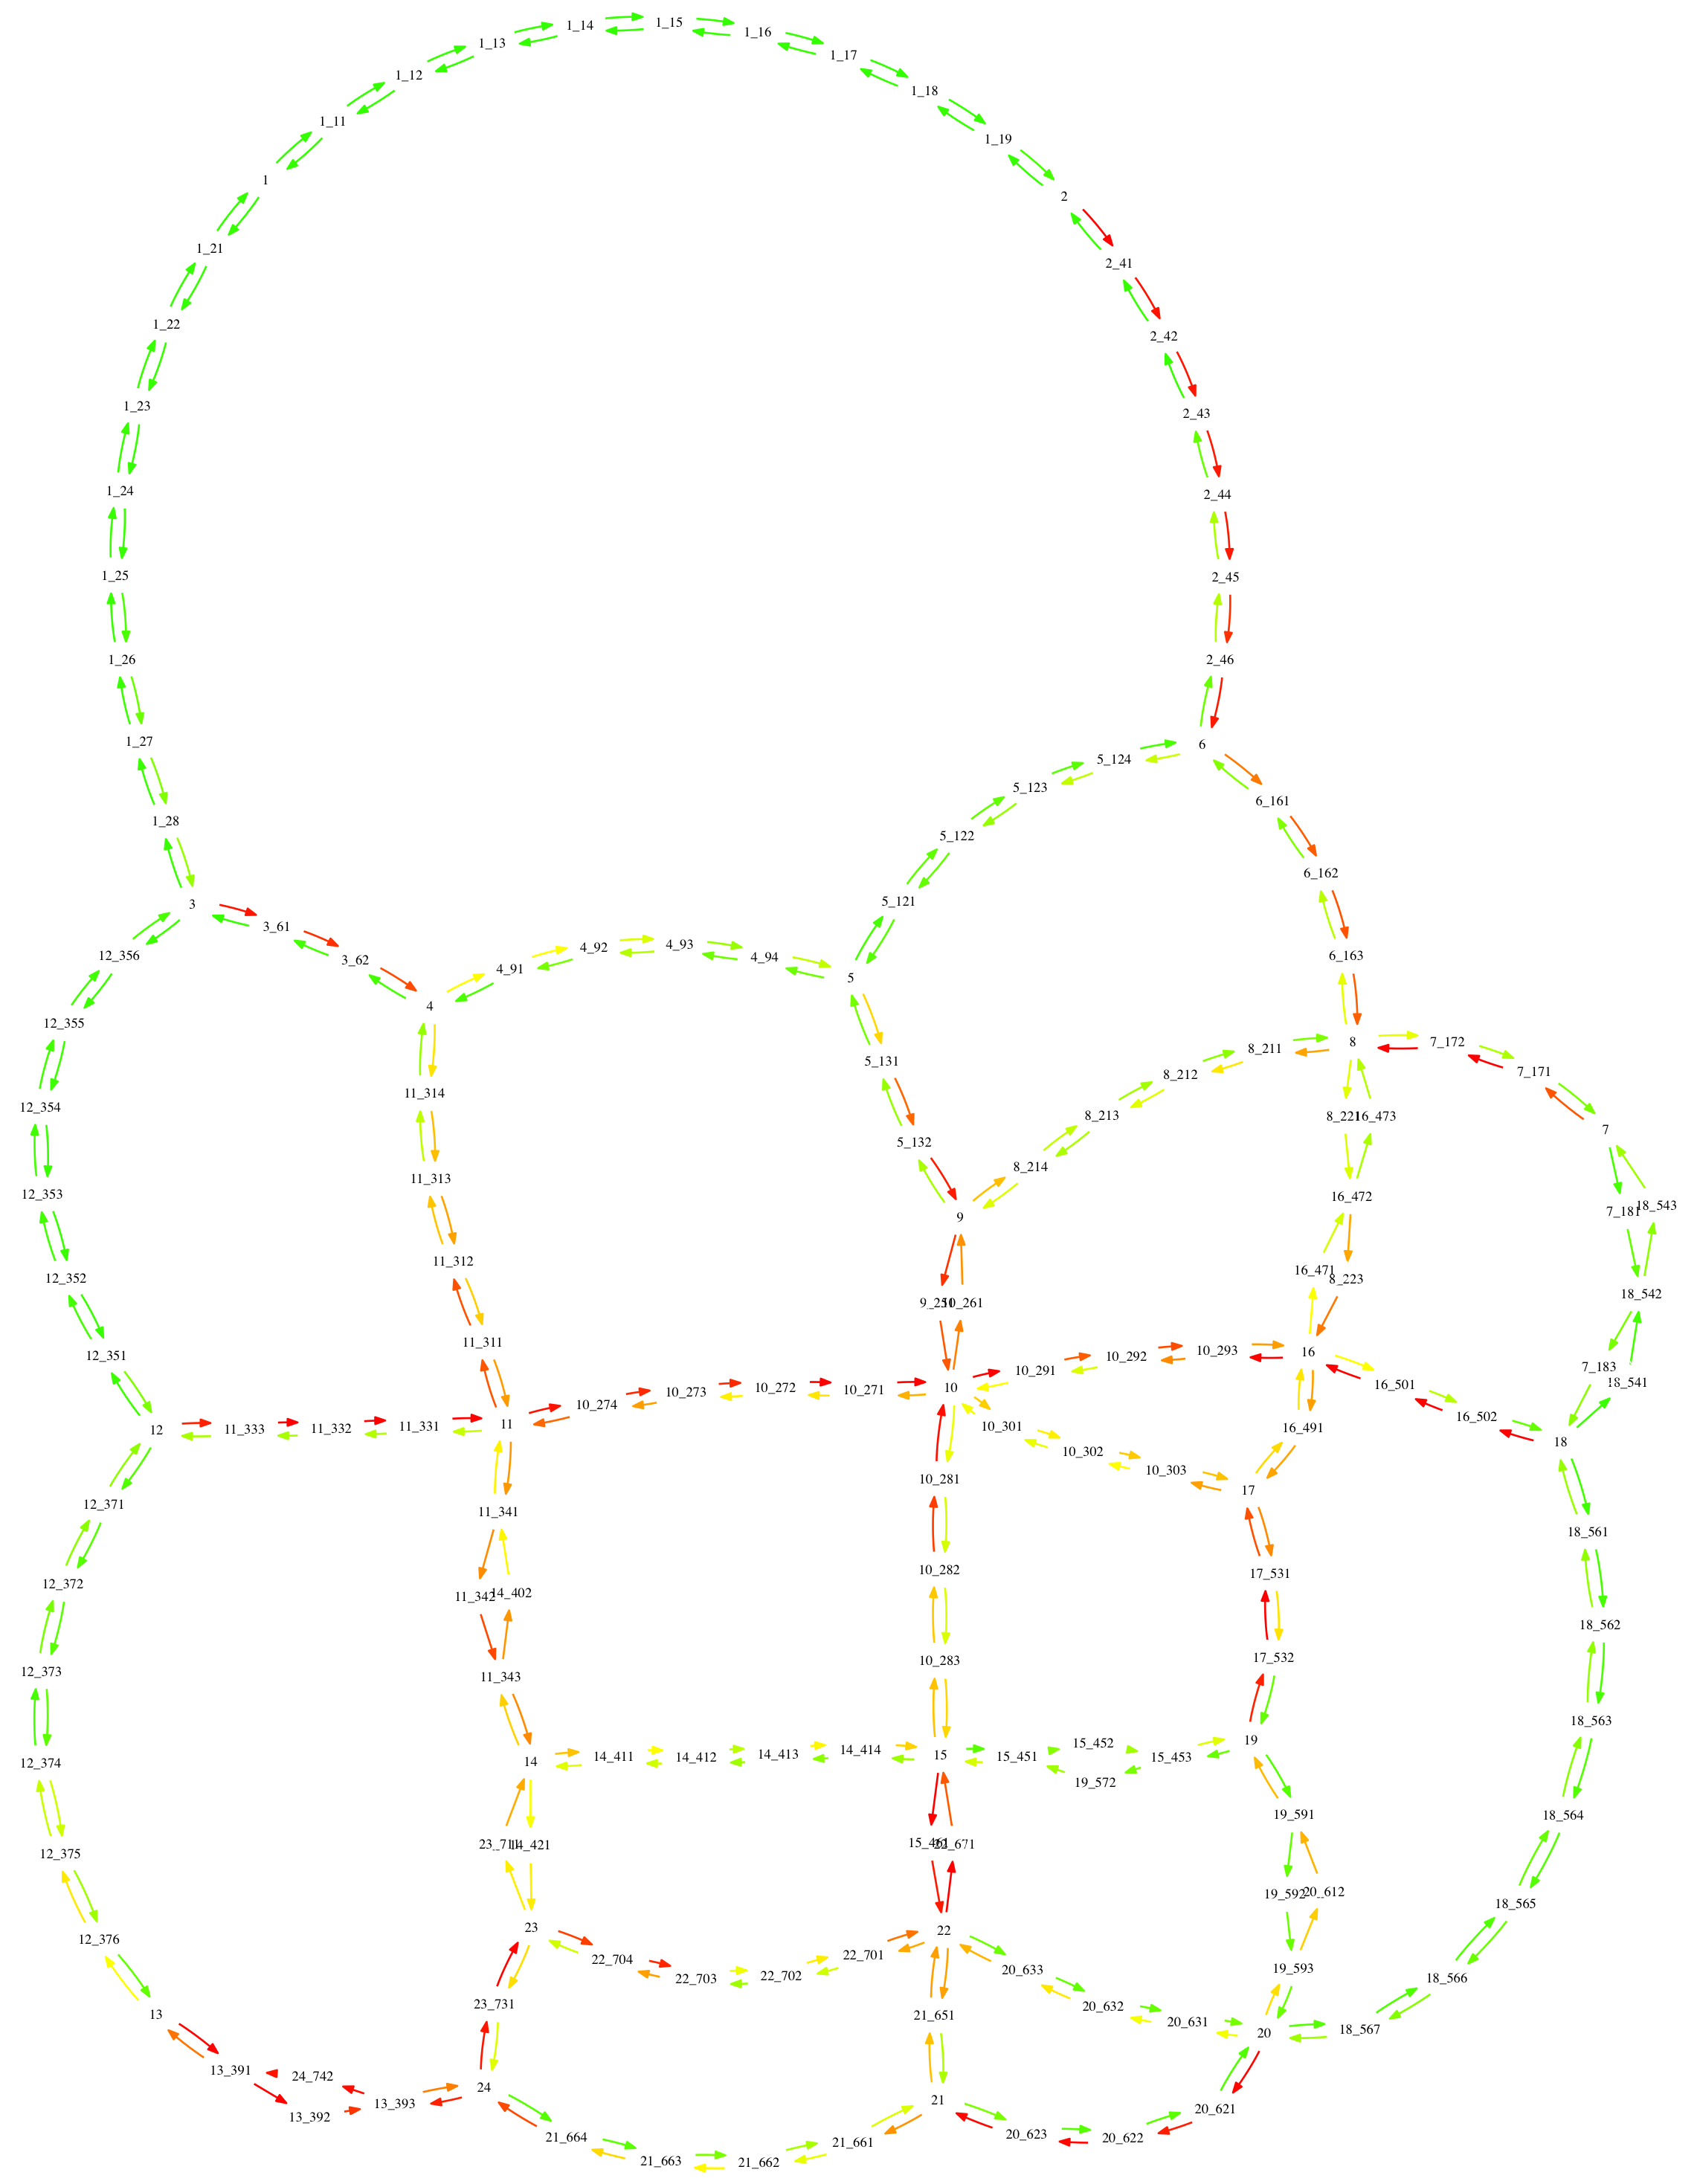
\includegraphics[totalheight=0.560\textheight, angle=90]{{{img/sioux/graph6.00-7.00}}}
\caption{Natężenie ruchu w mieście Sioux Falls w godzinach 6.00-7.00.} 
\label{ex-sioux-1}
\end{figure}

\begin{figure}[ht]
\centering
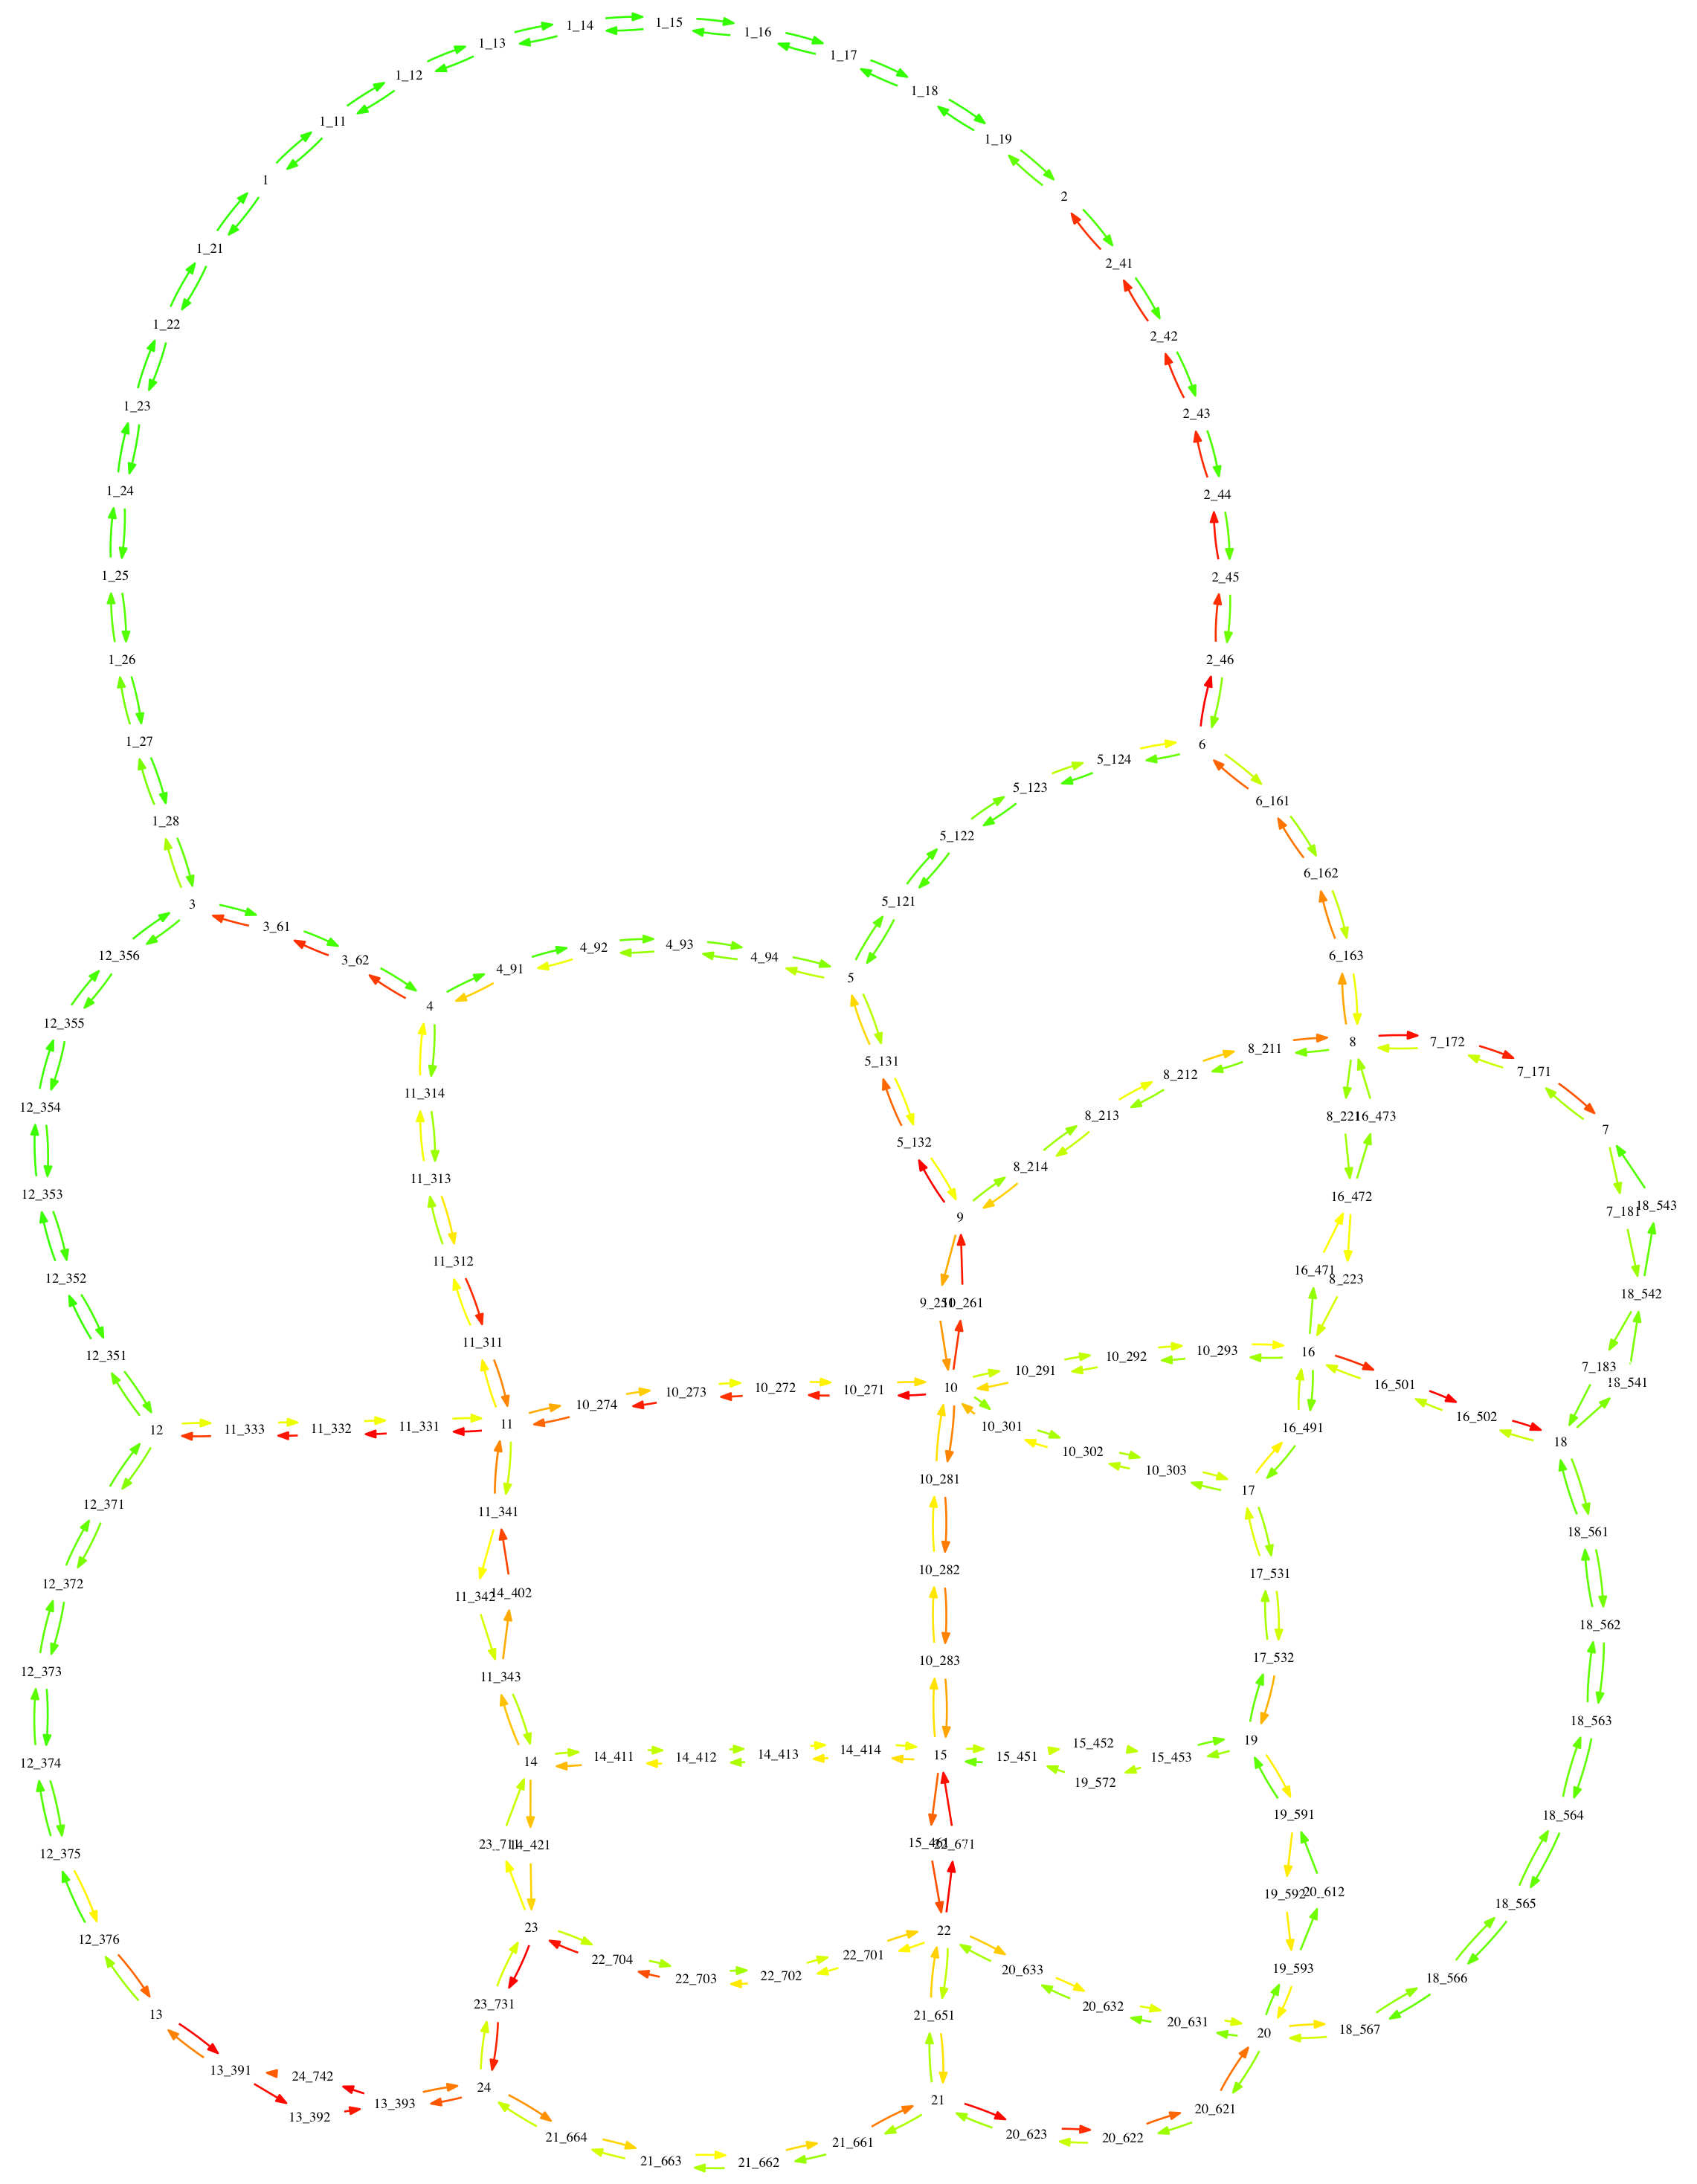
\includegraphics[totalheight=0.560\textheight, angle=90]{{{img/sioux/graph16.00-17.00}}}
\caption{Natężenie ruchu w mieście Sioux Falls w godzinach 16.00-17.00.} 
\label{ex-sioux-3}
\end{figure}

\clearpage
\section{Ustawienia symulatora.}\label{ukt}

Ostatnią ważną kwestią przed realizacją samego zadania optymalizacji jest dobór jego ustawień.~Część z~nich jest oczywiście stała lub nie ma wpływu bezpośrednio na obliczenia. Kluczową rolę dla ostatecznego wyniku odgrywają jednak parametry samej symulacji.

Większość ustawień została niezmieniona, pochodzi więc od twórców przykładu Sioux Falls. Symulator zawiera jednak ważny parametr ilości iteracji. Zgodnie z~założeniami symulatora, podczas każdej kolejnej iteracji, celem agenta jest zwiększenie jego średniego wyniku. Dąży on zatem do optymalizacji swoich planów dnia względem warunków na drodze. Przekłada się to bezpośrednio również na średni czas podróży każdego agenta. Twórcy zalecają stosowanie wysokich liczb iteracji, dla uzyskania jak najlepszych wyników, operacje te są jednak czasochłonne. Na rysunku \ref{def_stopwatch} przedstawiony został graf czasu uruchomienia symulacji jednej sieci dla stu iteracji. Podczas symulacji wykorzystywana była domyślna sieć miasta.

\begin{figure}[ht]
\centering
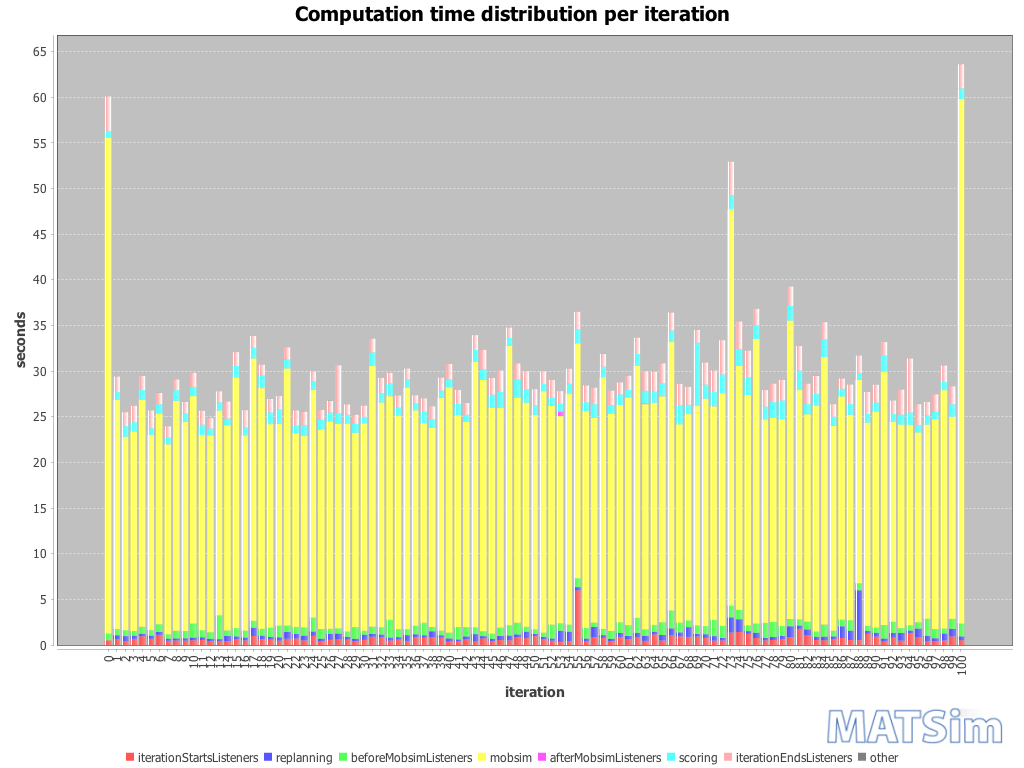
\includegraphics[width=0.85\textwidth]{img/def_stopwatch}
\caption{Graf czasu trwania symulacji MATSim dla stu iteracji.}
\label{def_stopwatch}
\end{figure}

Analizując wykres na rysunku \ref{def_stopwatch}, możemy odczytać czasy trwania kolejnych iteracji, jak również czas całej symulacji, który wyniósł dokładnie $52$min.~$43$sek.  W~przypadku analizy wielu (setek) sieci, czas więc jest wyraźnie zbyt długi. Przeanalizowaliśmy wpływ ilości iteracji na średni czas przejazdu, rysunek \ref{def_iters}. Średni wynik\footnote{ang. score} uzyskany przez agentów został natomiast przedstawiony na rysunku \ref{def_scorestats}.


\begin{figure}[ht]
\centering
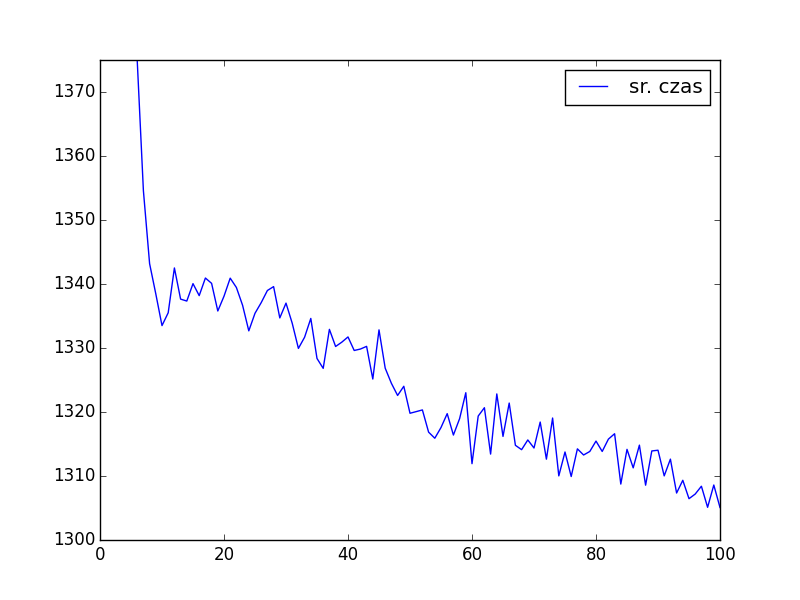
\includegraphics[width=0.85\textwidth]{img/def_iters}
\caption{Graf średniego czasu przejazdów dla stu iteracji.}
\label{def_iters}
\end{figure}

\begin{figure}[ht]
\centering
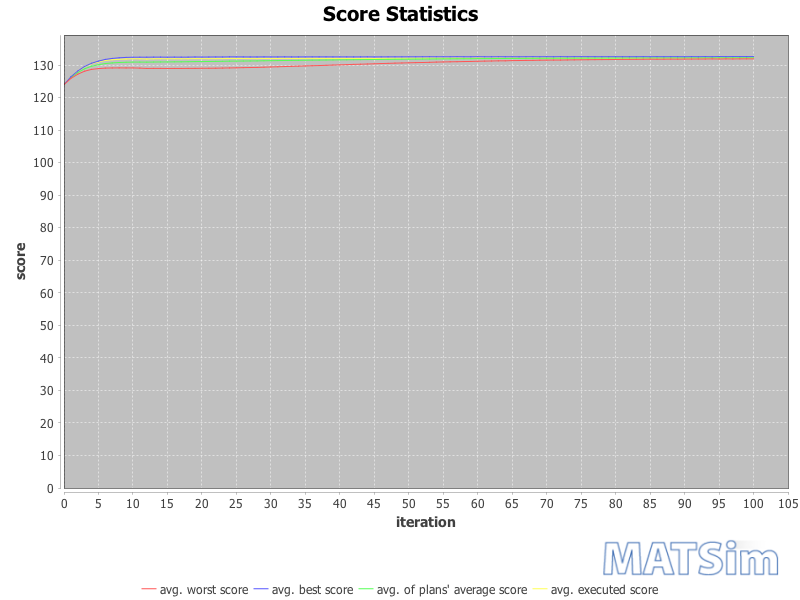
\includegraphics[width=0.85\textwidth]{img/def_scorestats}
\caption{Graf wyników agentów dla stu iteracji.}
\label{def_scorestats}
\end{figure}

Na wykresach \ref{def_iters} i~\ref{def_scorestats}, widać, że wpływ iteracji, ma największe znaczenie w~początkowych stadiach. W~późniejszych iteracjach zmiana następuje dużo wolniej.

Po analizie wykresów prezentowanych w~sekcji \ref{ukt}, zdecydowaliśmy w~projekcie na użycie $10$ iteracji podczas analizy każdej sieci. Wartość ta optymalnie łączy zalety szybkiego spadku wartości średnich czasów podróży i~czasu potrzebnego na obliczenia.

\section{Ustawienia projektu.}

Podczas badań wykorzysaliśmy ustawienia algorytmu genetycznego zgodne z~listingiem \ref{geneconf}. Wartości zostały dobrane na podstawie doświadczenia nabytego w~trakcie studiów literaturowych. 
	
\begin{lstlisting}[caption=Ustawienia algorytmu genetycznego podczas badań.,label=geneconf]
<genetics>
	<population-size>24</population-size>
	<max-generations>200</max-generations>
	<elitism-rate>2.0</elitism-rate>
	<crossover-rate>1.0</crossover-rate>
	<mutation-rate>0.8</mutation-rate>
	<tournament-arity>4</tournament-arity>
</genetics>
\end{lstlisting}

\clearpage
\section{Wyniki.}

Wykres przedstawiający zestawienie wyniku najlepszej sieci wyłonionej w~danej iteracji, do wyniku sieci wejściowej przedstawiamy na rysunku \ref{def_fitness}.

\begin{figure}[ht]
\centering
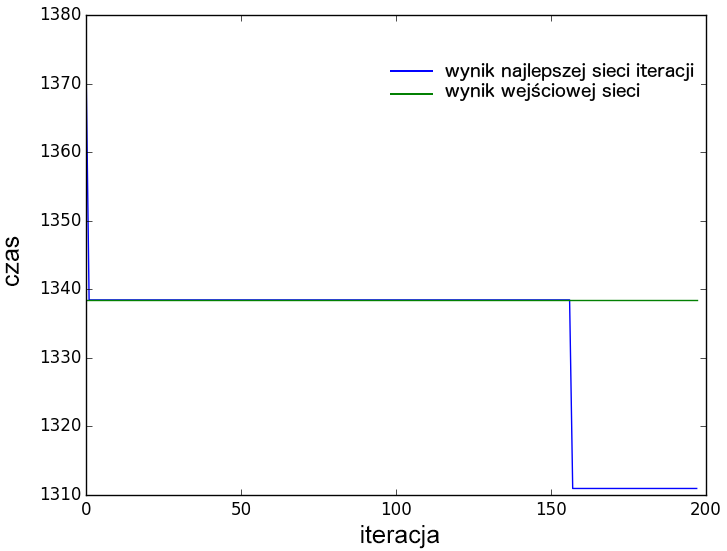
\includegraphics[width=0.85\textwidth]{img/fitness}
\caption{Graf wyników algorytmu genetycznego.}
\label{def_fitness}
\end{figure}

Ponieważ w~projekcie wykorzystany został elitystyczny model populacji algorytmu genetycznego, powyższy wykres nie przedstawia praktycznie żadnych zmian w~populacji, która została ulepszona. Wyniki wszystkich chromosomów były jednak zachowywane w~bazie. Dzięki temu możemy przedstawić więcej sieci spełniających założenia projektowe.

Najlepsze wyniki symulacji przedstawiamy w~tabeli \ref{tab_best}. Przedstawione są tutaj wszystkie sieci, które uzyskały wynik lepszy od sieci wejściowej, tj. $1338.4505528474617$. Od teraz, będziemy odnosić się do tych sieci używając ich numeru identyfikacyjnego (pierwsza kolumna).

\begin{minipage}{\linewidth}
\captionof{table}{Zbiór najlepszych otrzymanych sieci.}
\label{tab_best} 
\begin{tabularx}{\linewidth}{ | l | X | r | }
	\hline
	ID & Reprezentacja binarna & Wynik sieci \\
	\hline
	1 & 011111111111111111111111111111111111111111111 	111111111111111111111111111111111111110111111 & 1310.95255617644 \\ \hline
	2 & 011111111111111111111111011111110111111111111 111111111111111111111111111111111111110111111 & 1312.64143383664 \\ \hline
	3 & 011111111111111111111111111111111111111111111 111111111111111111110111111111111111110111111 & 1312.73299250981 \\ \hline
	4 & 011111111111111111111111111111110111111111111 111111111111111111111111111111111111110111111 & 1313.75345975508 \\ \hline
	5 & 011111111111111111111111111111111111111111111 111111111111111111111111111111111111110111101 & 1318.77194744977 \\ \hline
	6 & 011111111111111111111111011111111111111111111 111111111111111111111111111111111111110111111 & 1320.54353227916 \\ \hline
	7 & 011111111111111111111111111111111111111111111 111111111111111111111111111111111111110110111 & 1322.64708120319 \\ \hline
	8 & 011111111111111111111111011111111111111111111 111111111111111111110111111111111111110111111 & 1323.53190464867 \\ \hline
	9 & 011111111111111111111111111111111111111111111 111111111111111111111111111111111111110111110 & 1325.07095470218 \\ \hline
	10 & 01111111111111111111111111111111111111111111 1111111111111111111111110111111111111110111111 & 1327.94727737487 \\ \hline
	11 & 01111111111111111111111111111111111111111111 1111111111111111111111110111111111111110111101 & 1329.46298894305 \\ \hline
	12 & 01111111111111111111111101111111111111111111 1111111111111111111111110111111111111110111111 & 1332.87335631911 \\ \hline
	13 & 01111111111111111111111111111111111111111111 1111111111111111111111111111111111111110111011 & 1334.28138152419 \\ \hline
	14 & 01111111111111111111111111111111111111111111 1111111111111111111111111111111111110110111111 & 1334.48972773749 \\ \hline
	15 & 01111111111111111110111111111111111111111111 1111111111111111111111111111111111111110111111 & 1335.74516109856 \\ \hline
	16 & 01111111111111111111111111111111111111111111 1111111111111111111111111111111111111110111010 & 1335.96306027821 \\ \hline
	17 & 01111111111111111111111111111111111001111111 1111111111111111111111111111111111111110111111 & 1336.65051123529 \\ \hline
\end{tabularx}
\end{minipage}%

\newpage
Na rysunkach \ref{sioux1} - \ref{sioux17} prezentujemy grafy uzyskanych sieci, dla wizualizacji rozwiązań. \textbf{W celu uproszczenia odnajdowania usuniętych węzłów, są one zaznaczone kolorem czerwonym.} Tak, jak w~poprzednim przypadku, sieci zostały obrócone o~$90^{\circ}$ w~lewo. W~niektórych przypadkach wycięte węzły są trudno widoczne, z~powodu nikłej długości strzałki. Dotyczy to przede wszystkim przykładów: \ref{sioux5}, \ref{sioux7}, \ref{sioux9}, \ref{sioux10}, \ref{sioux11}, \ref{sioux12}, \ref{sioux13}, \ref{sioux14}, \ref{sioux16}. W~tych sieciach zostały wycięte drogi w~pobliżu węzła o~numerze $ 15$.

\begin{figure}[ht]
\centering
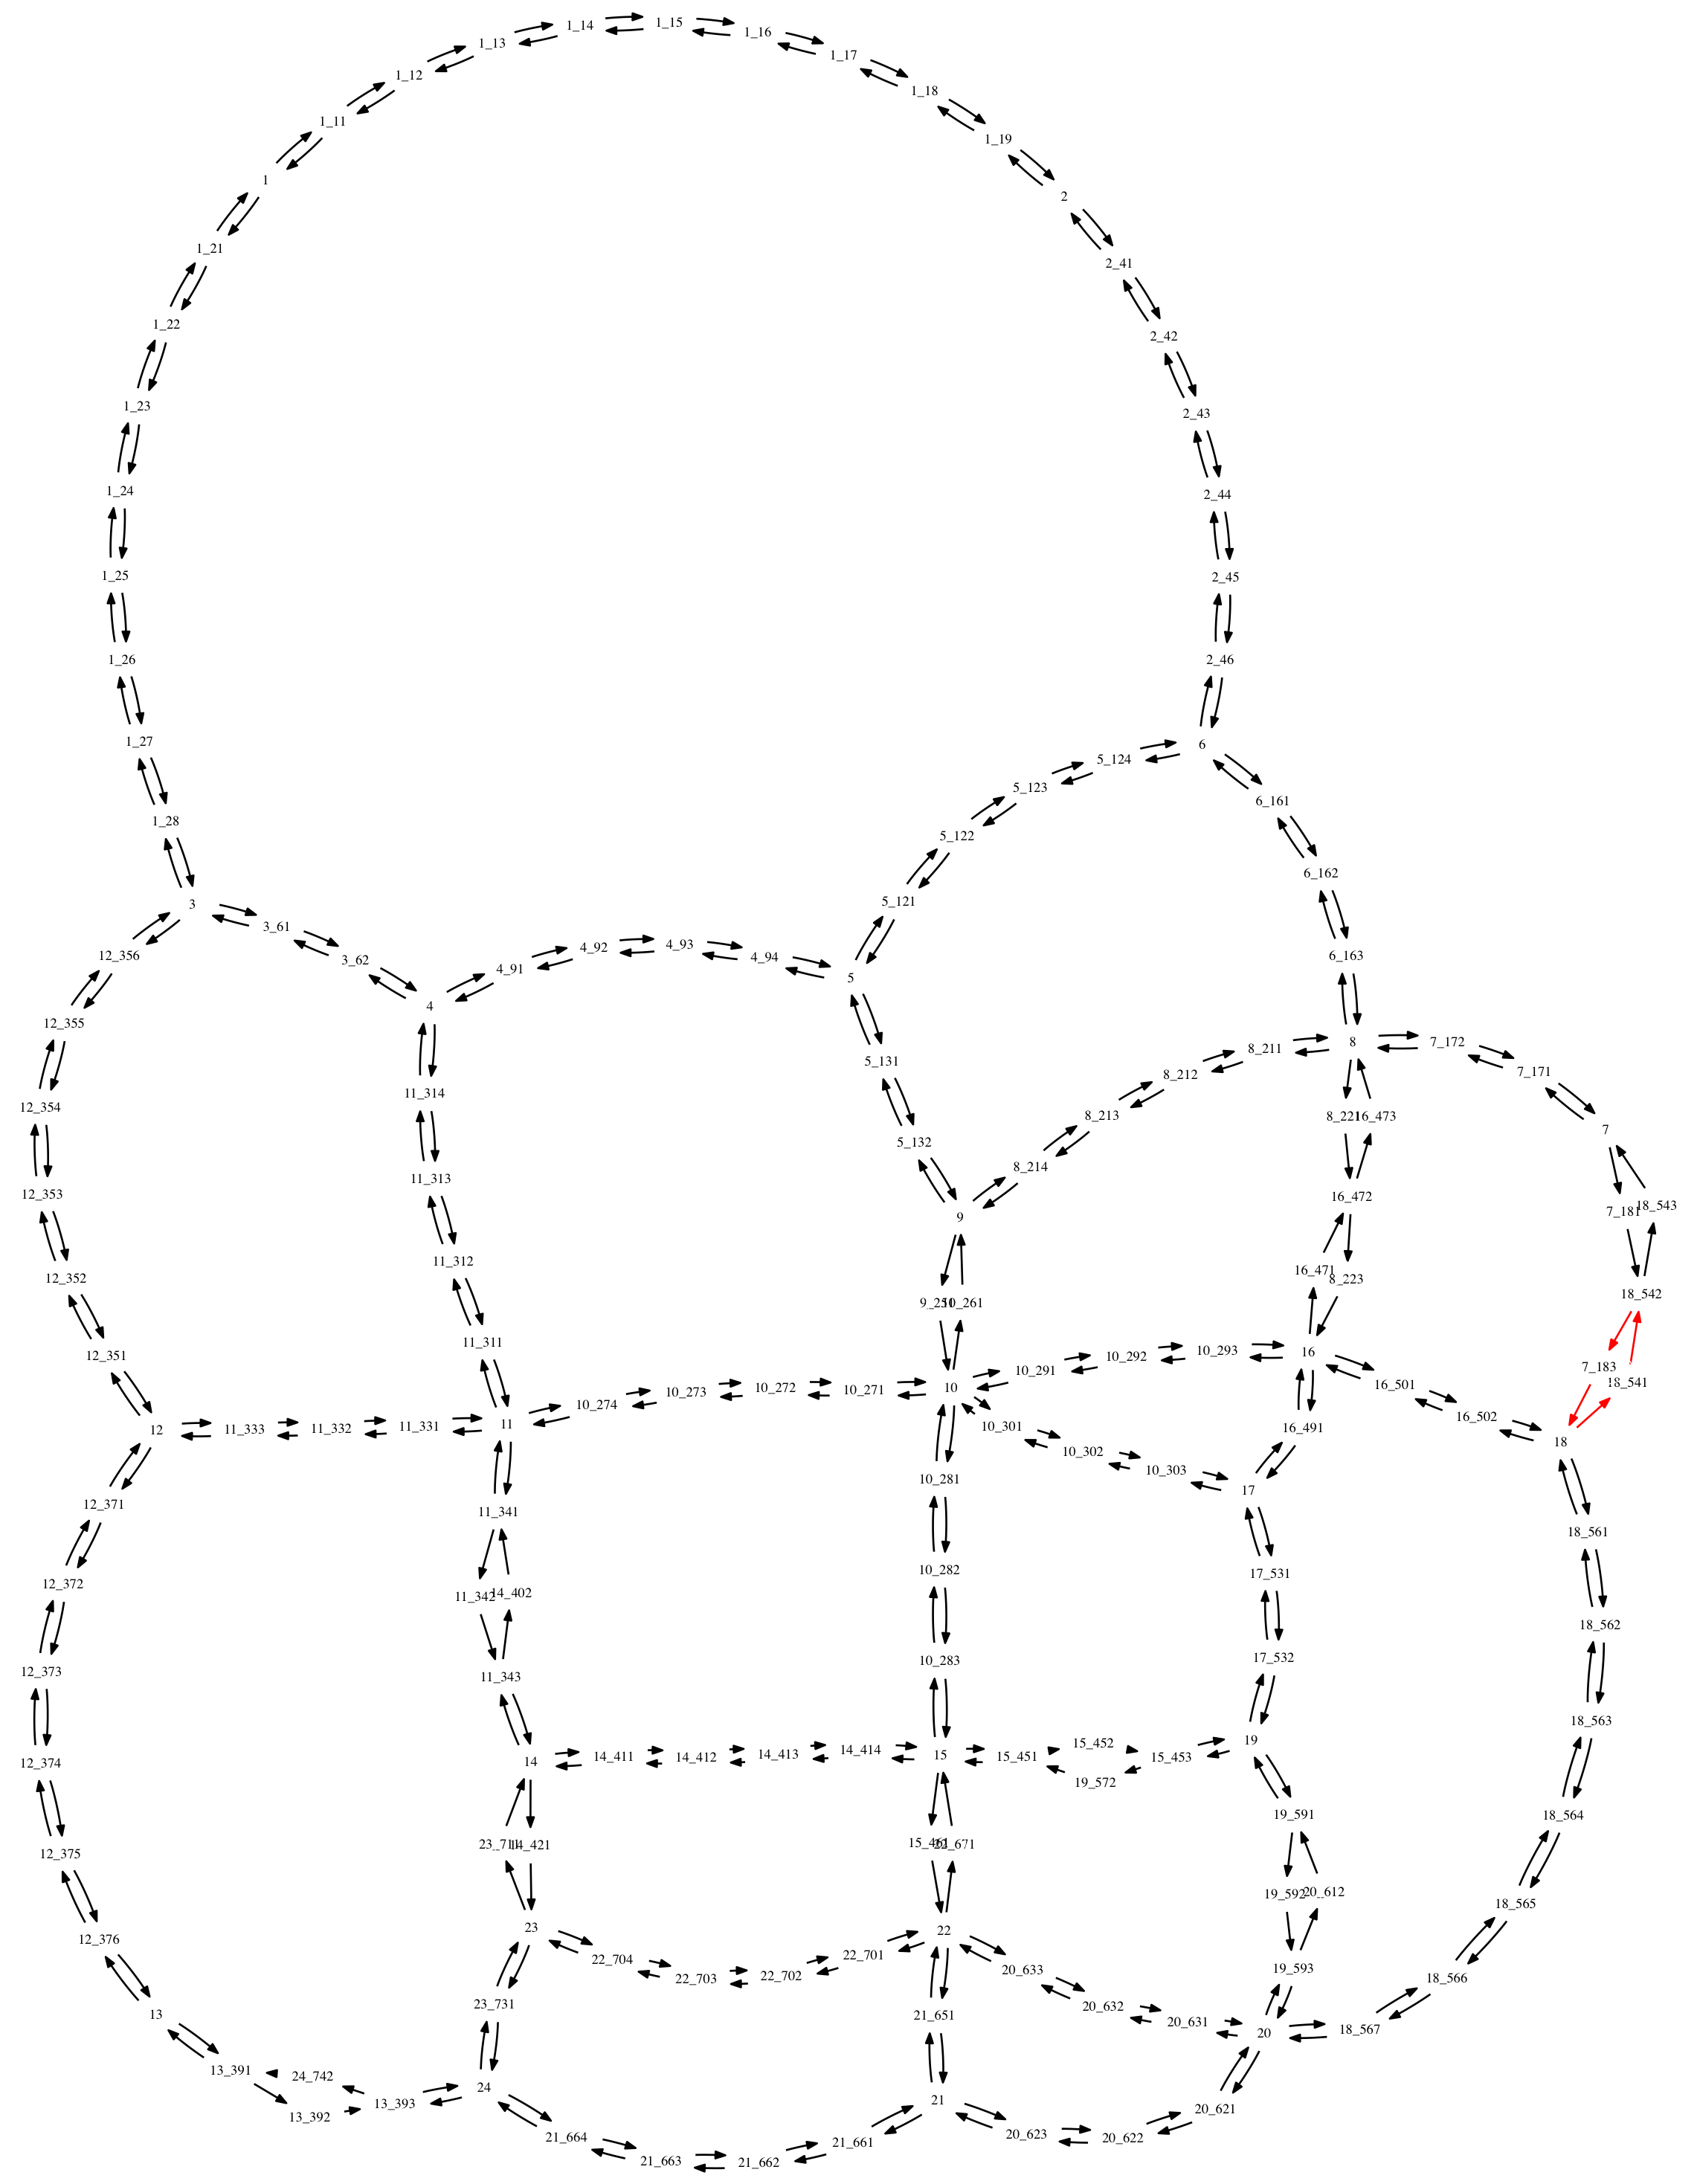
\includegraphics[totalheight=0.580\textheight, angle=90]{img/sioux-out/1/network2}
\caption{Sieć miasta Sioux Falls, rozwiązanie nr. 1.}
\label{sioux1}
\end{figure}

\begin{figure}[ht]
\centering
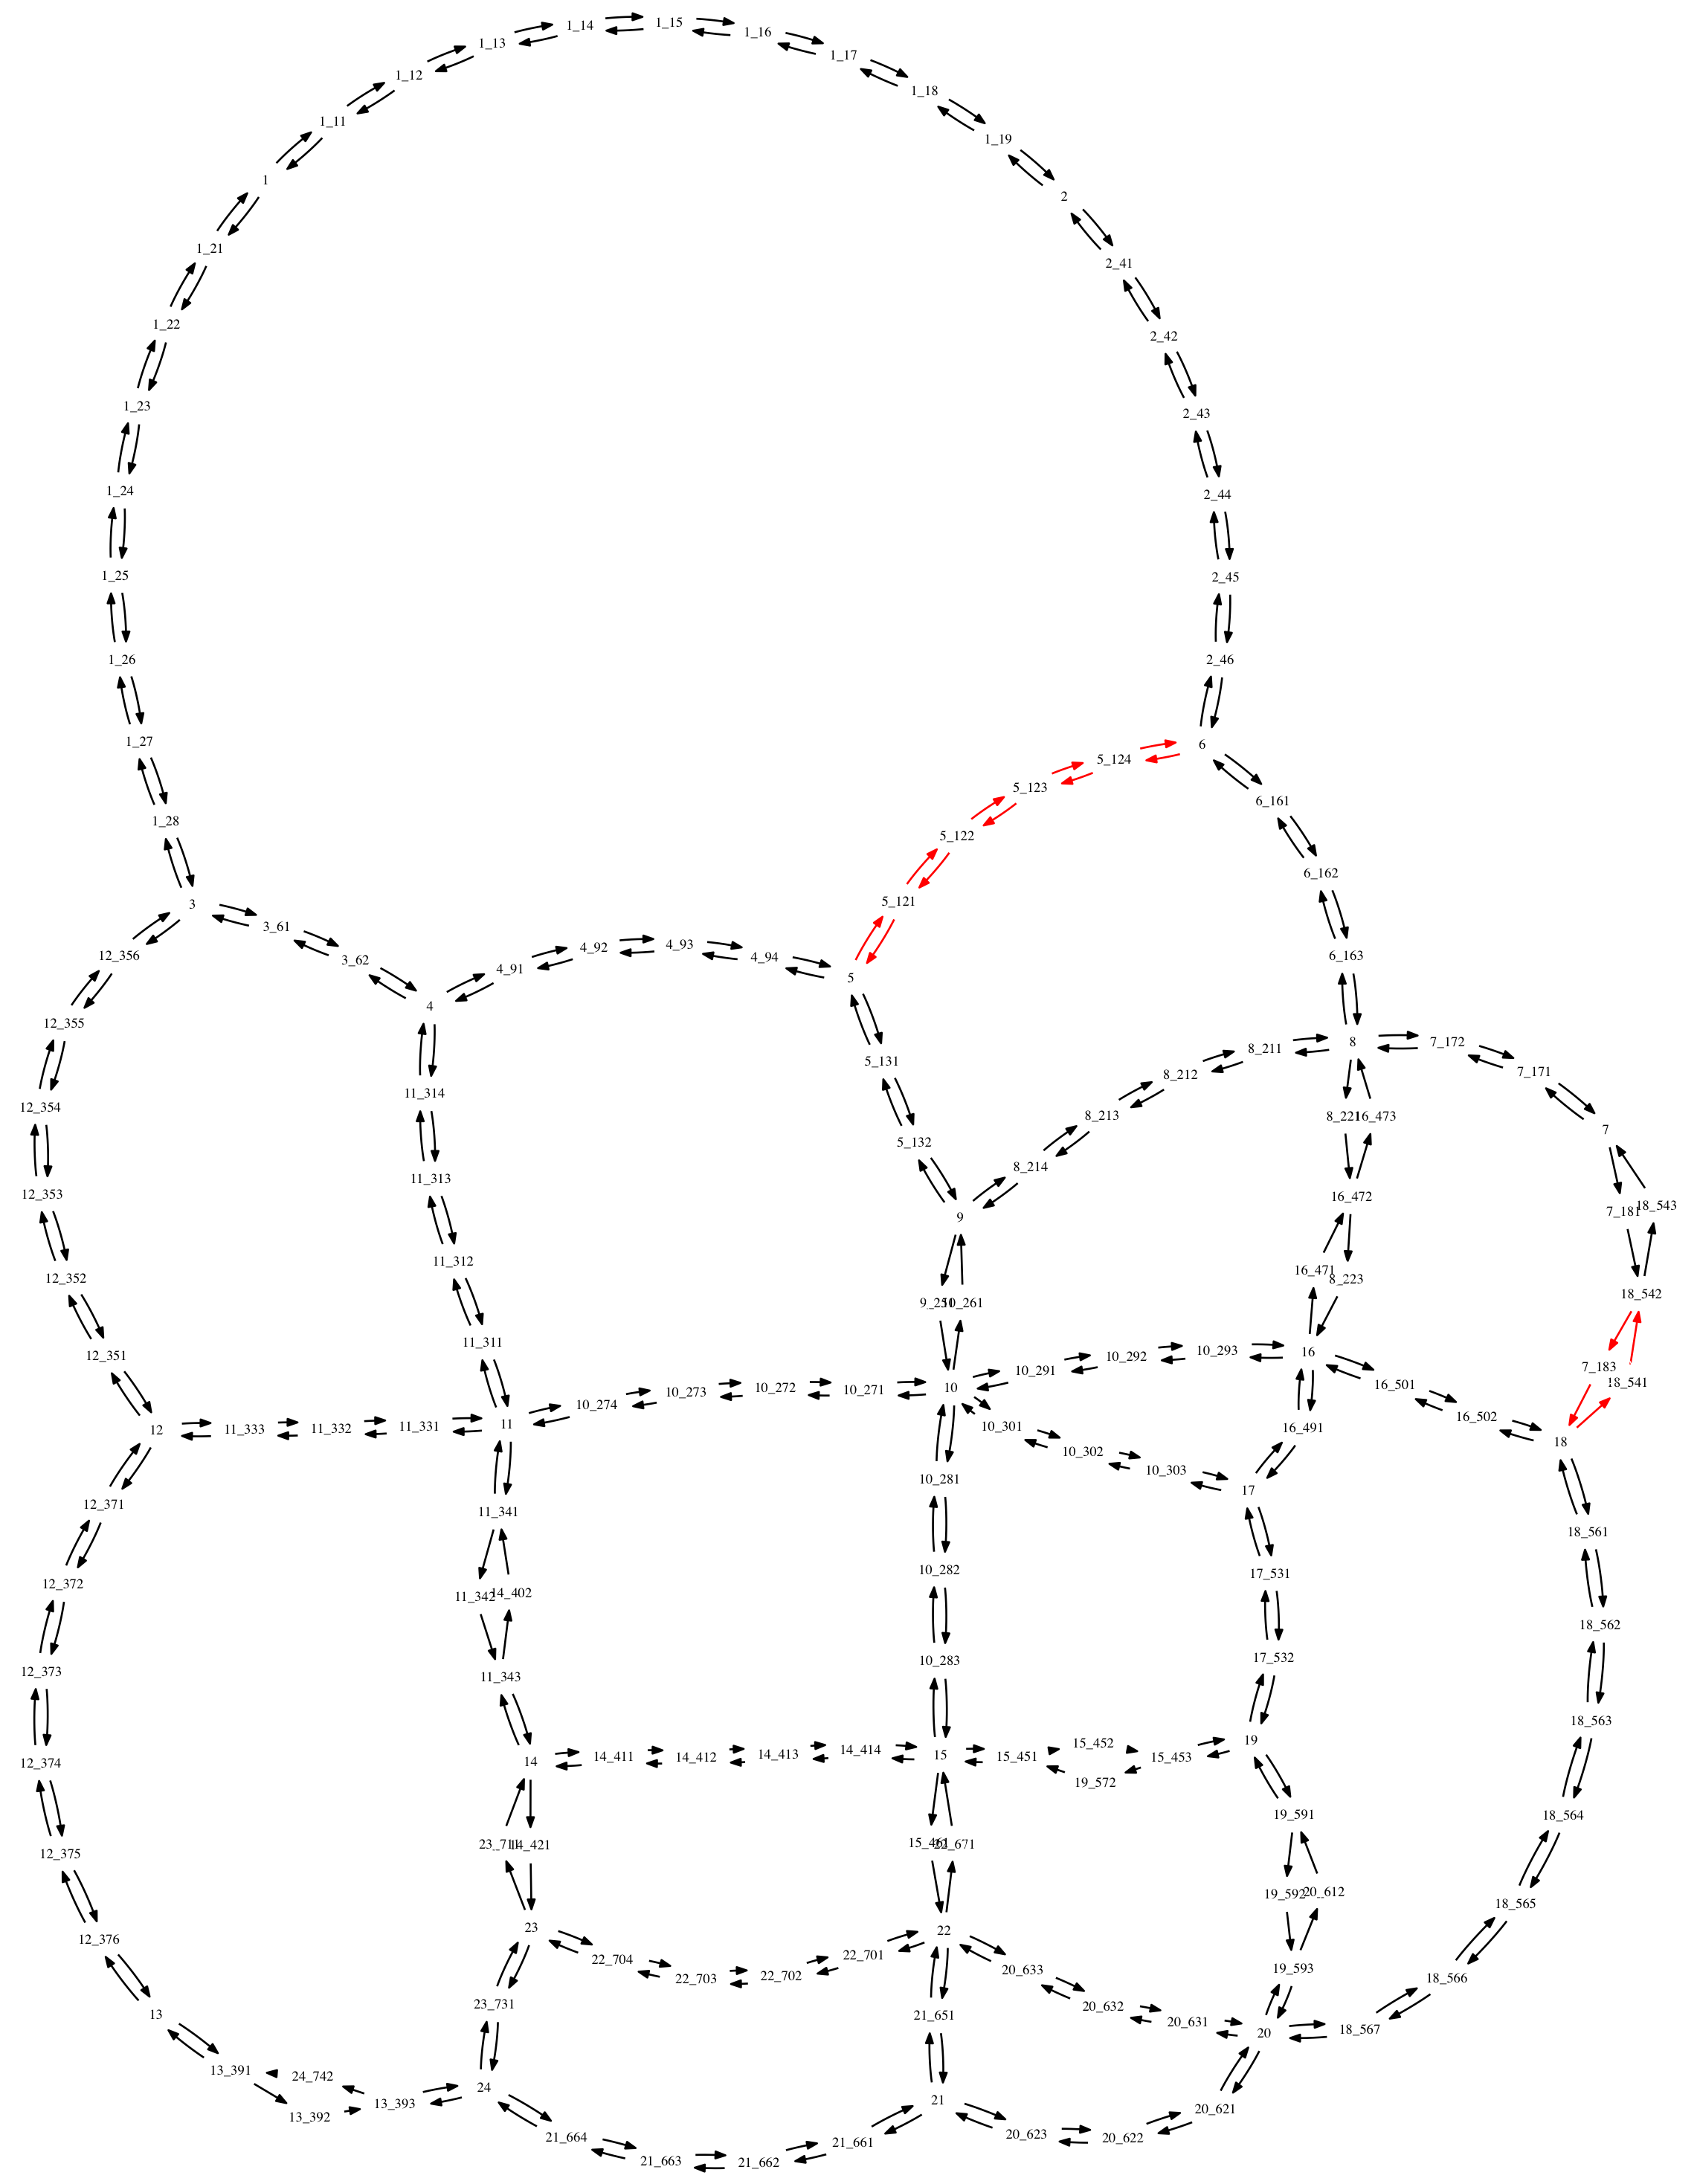
\includegraphics[totalheight=0.580\textheight, angle=90]{img/sioux-out/2/network2}
\caption{Sieć miasta Sioux Falls, rozwiązanie nr. 2.}
\label{sioux2}
\end{figure}

\begin{figure}[ht]
\centering
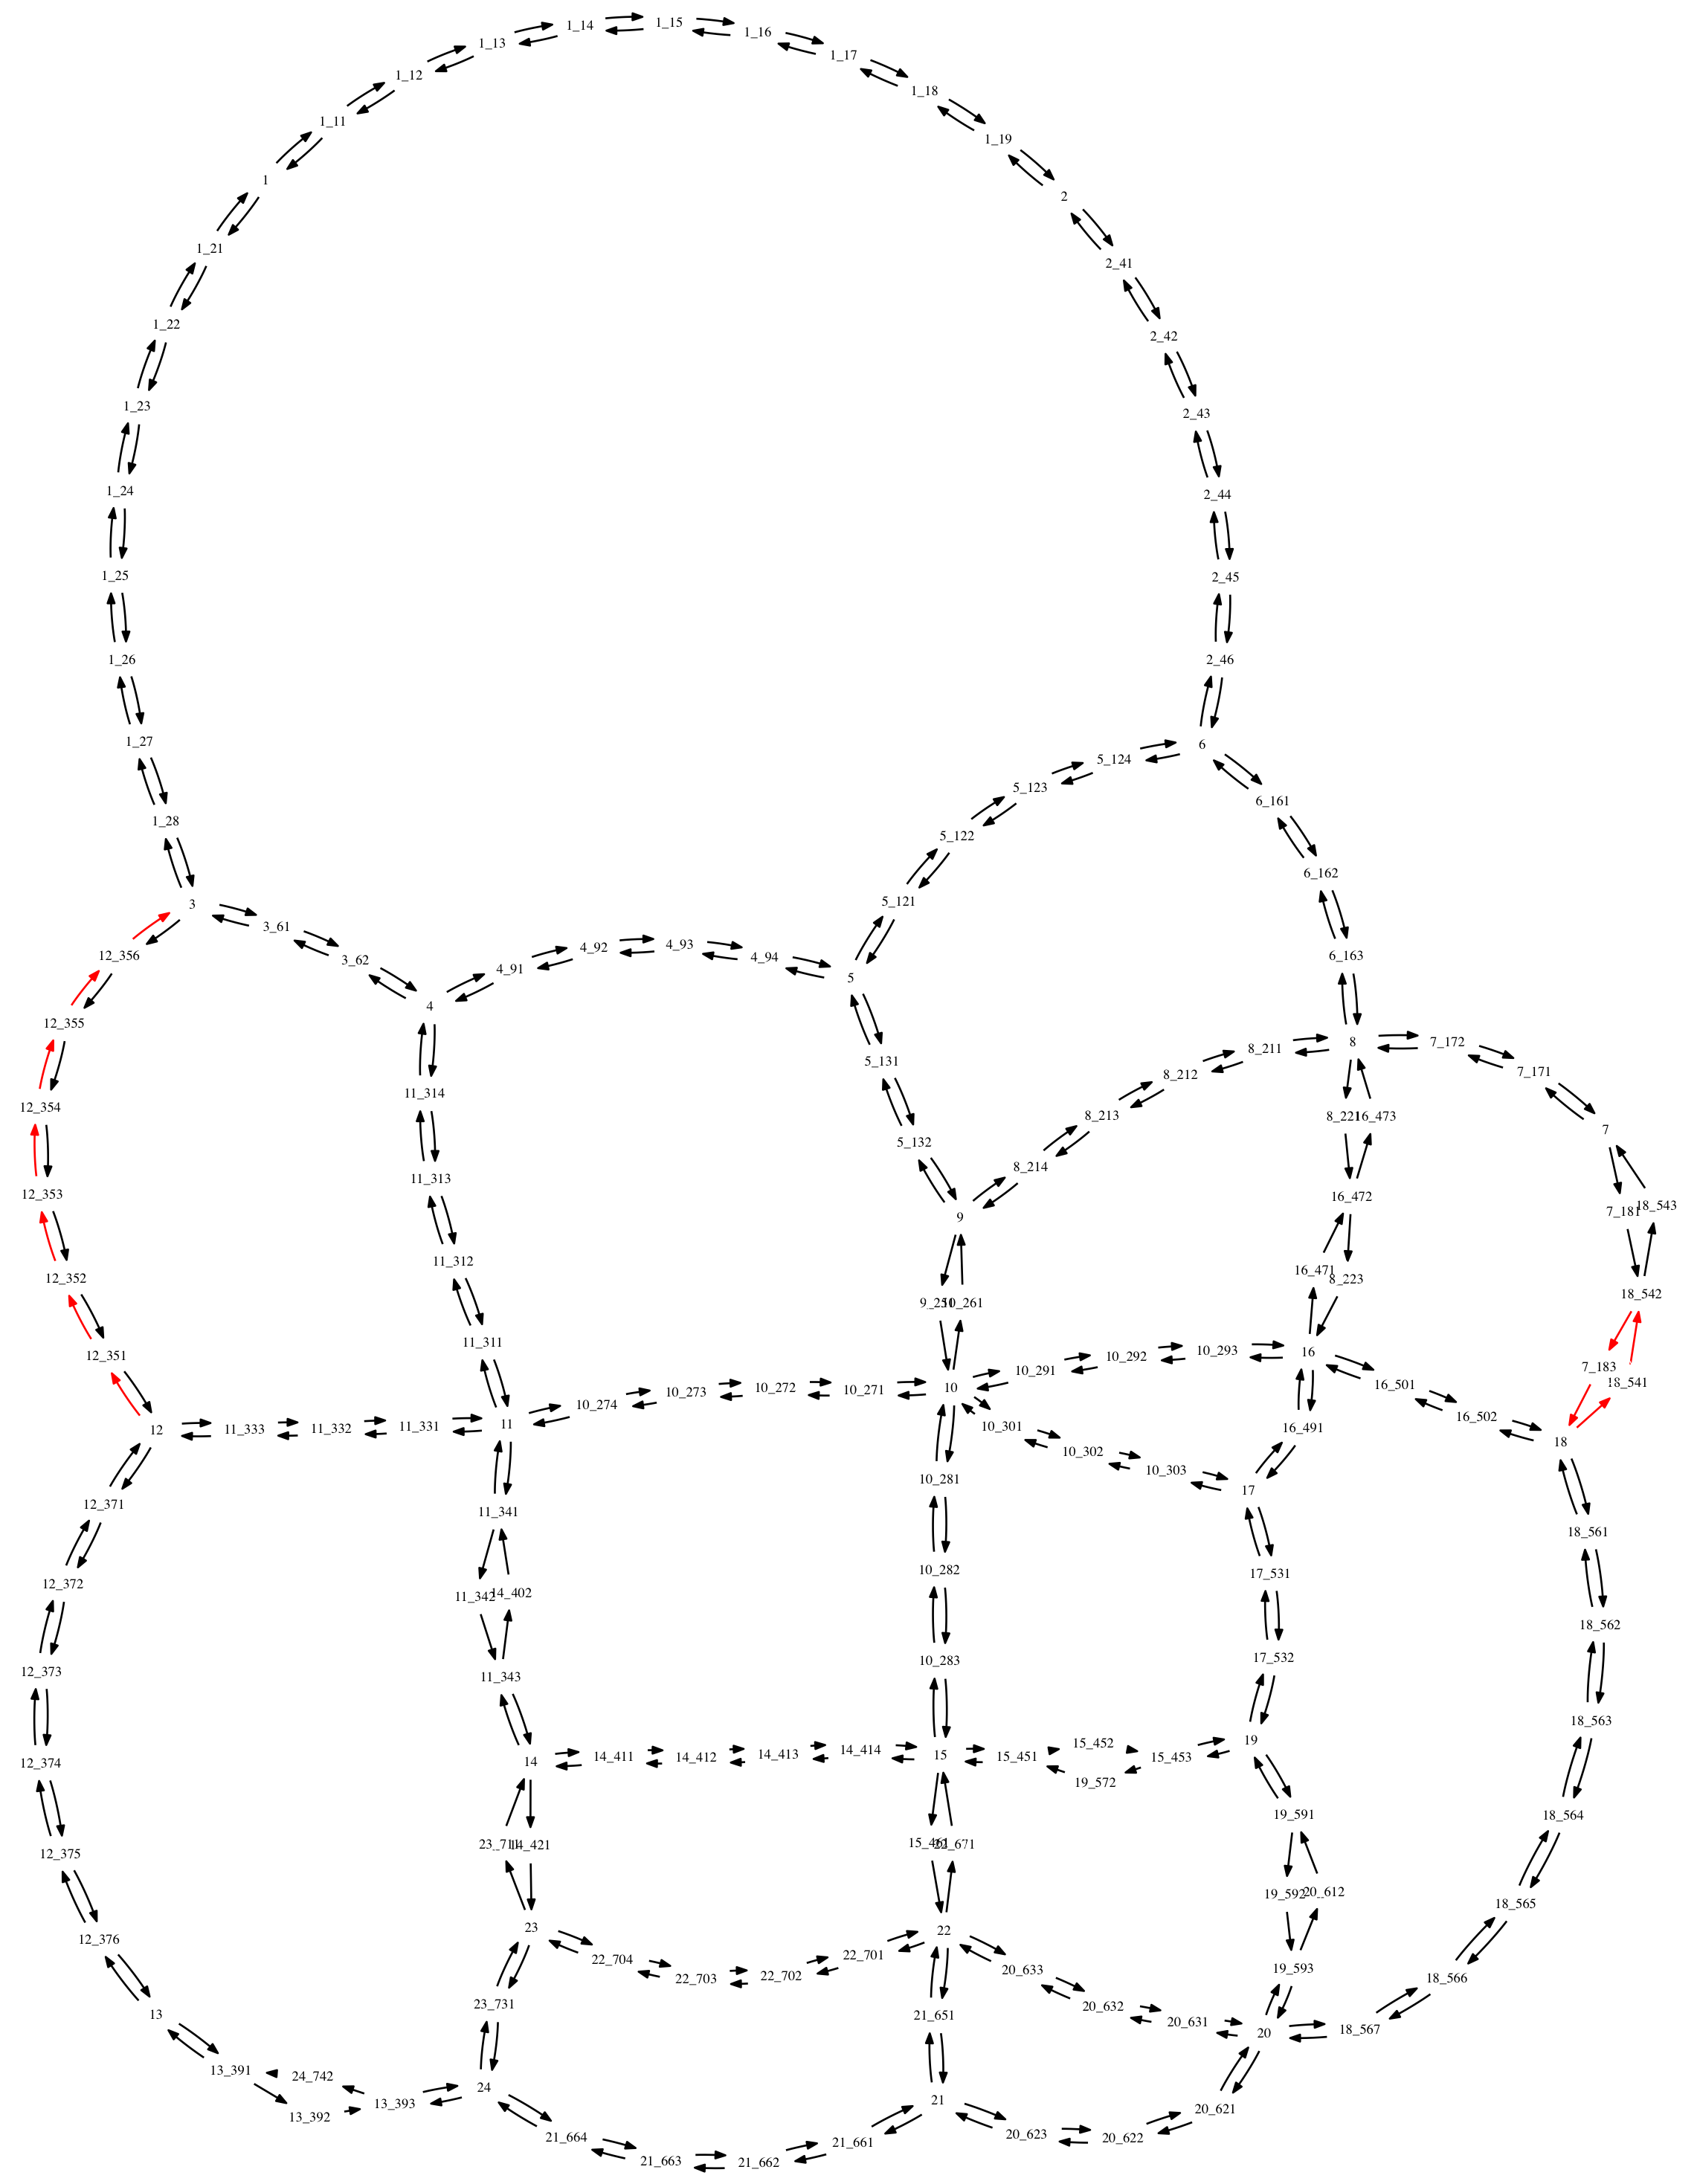
\includegraphics[totalheight=0.580\textheight, angle=90]{img/sioux-out/3/network2}
\caption{Sieć miasta Sioux Falls, rozwiązanie nr. 3.}
\label{sioux3}
\end{figure}

\begin{figure}[ht]
\centering
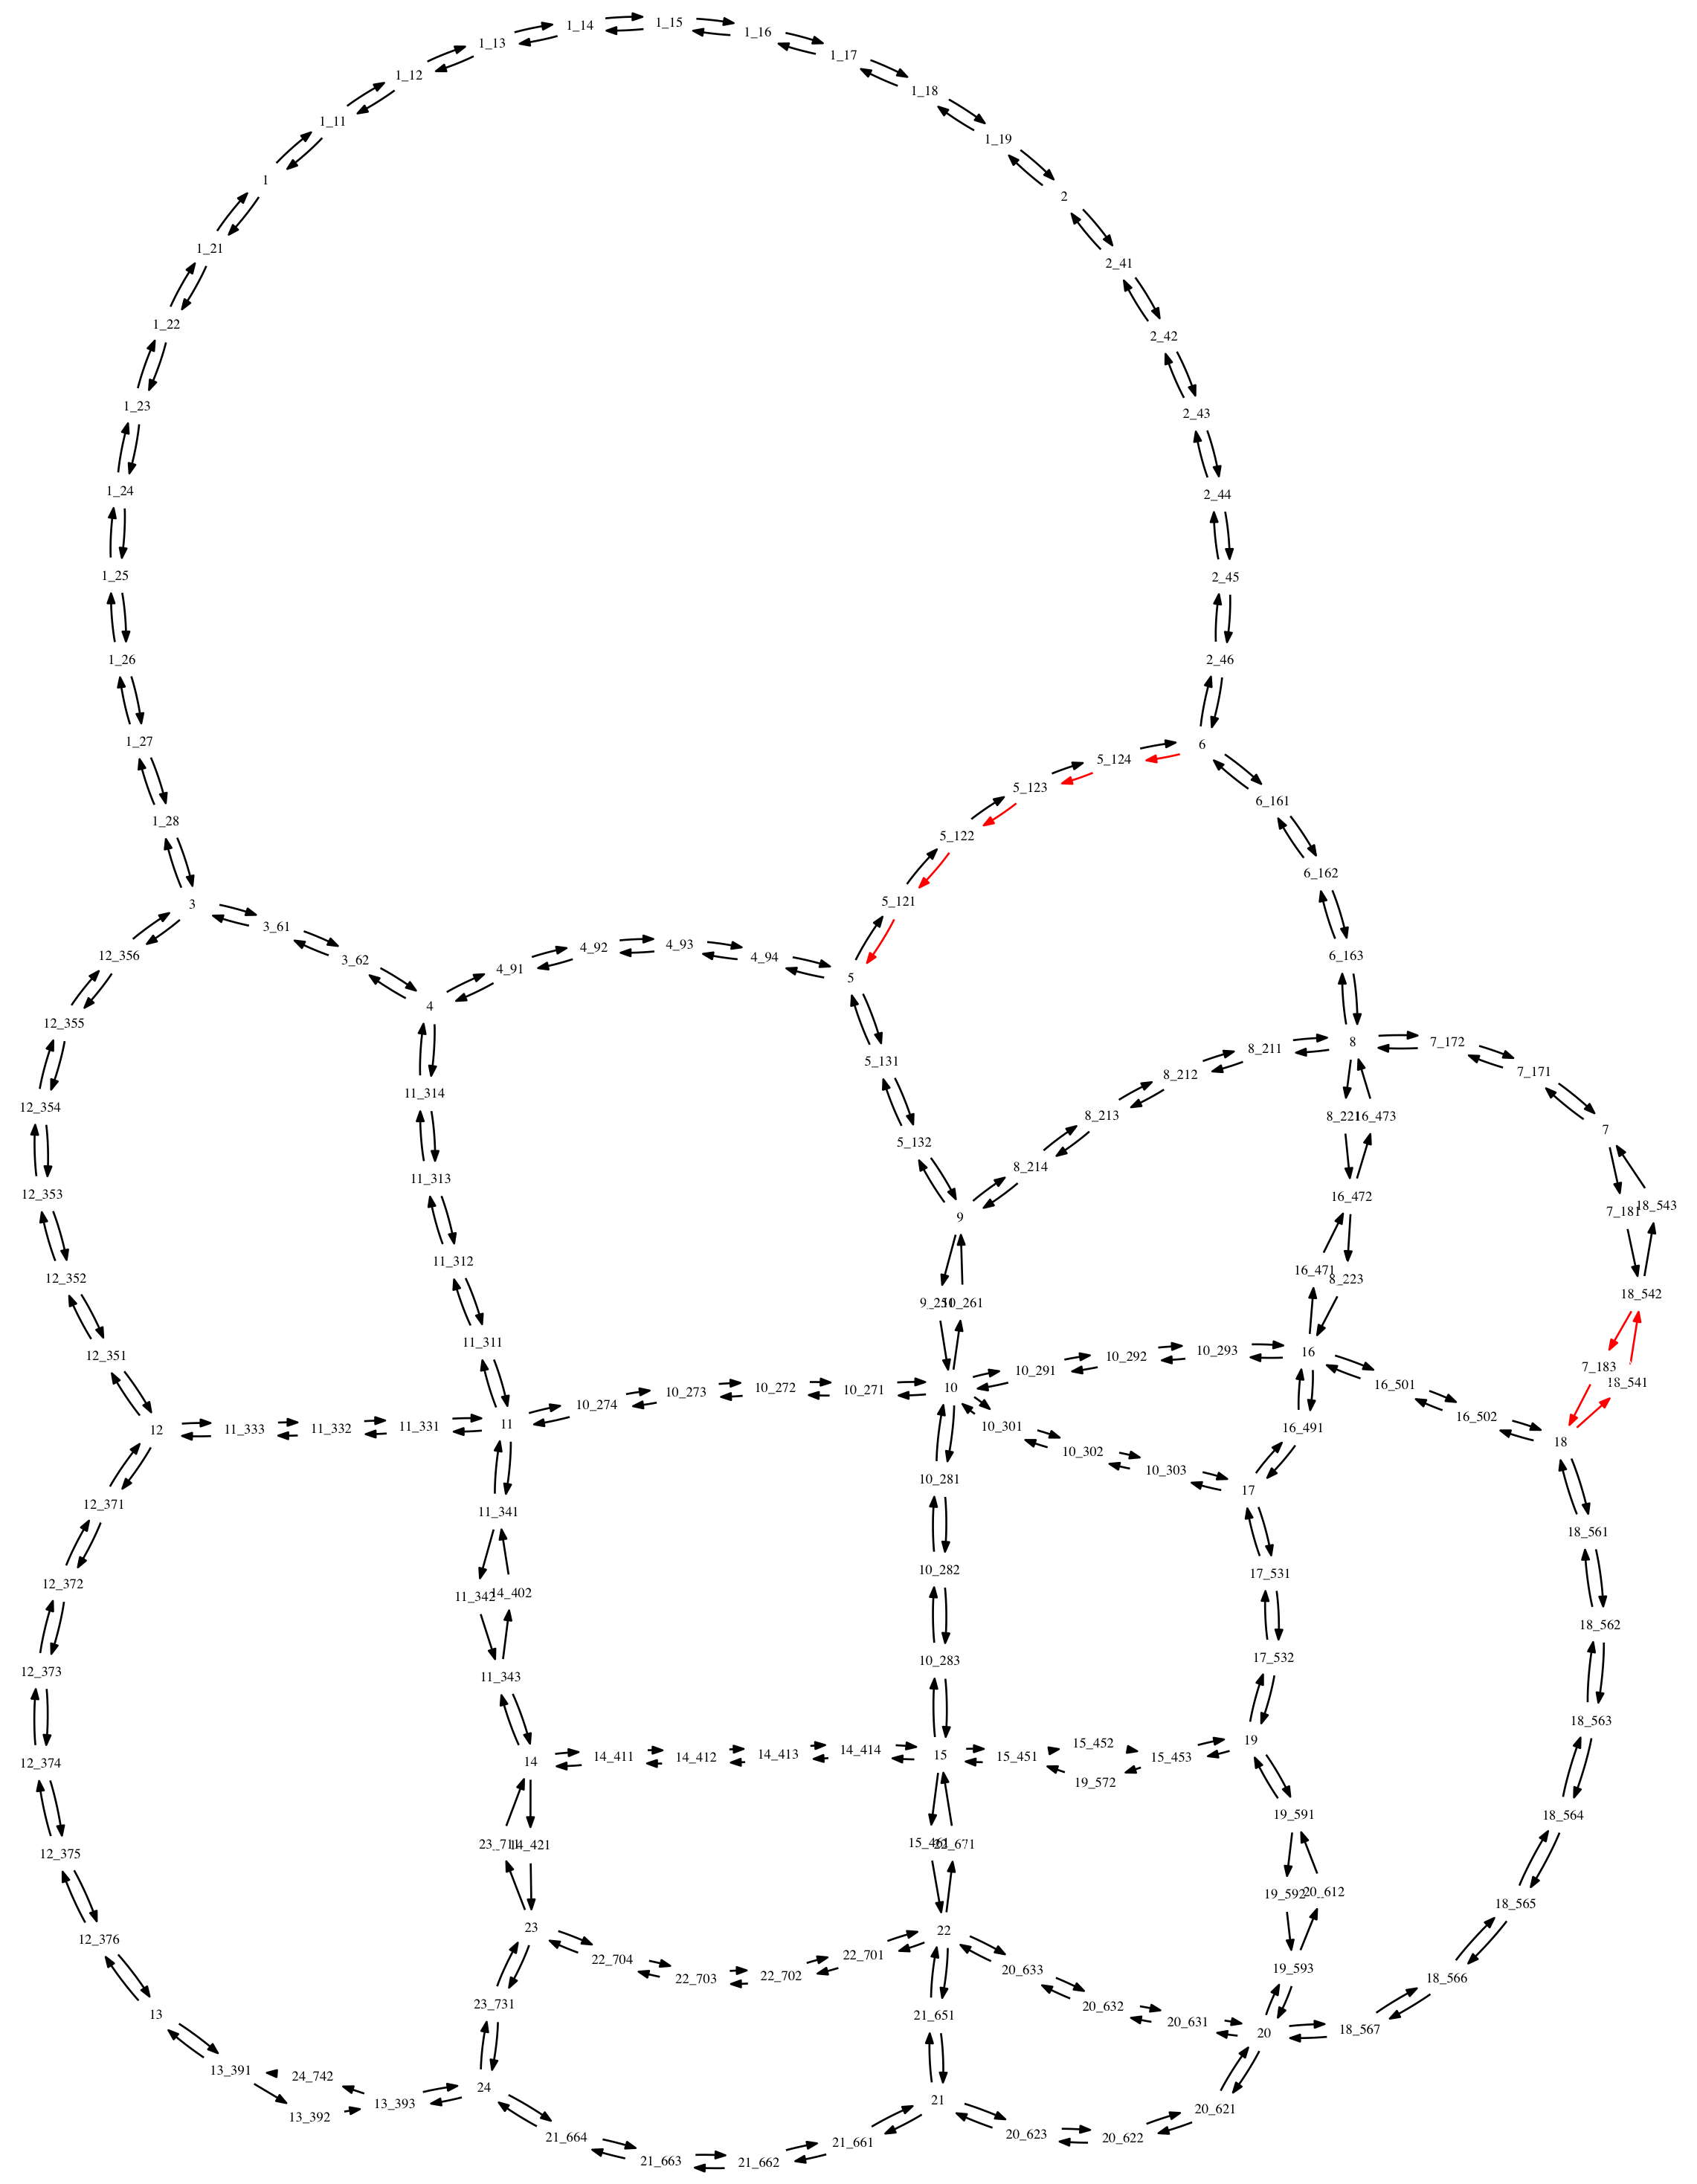
\includegraphics[totalheight=0.580\textheight, angle=90]{img/sioux-out/4/network2}
\caption{Sieć miasta Sioux Falls, rozwiązanie nr. 4.}
\label{sioux4}
\end{figure}

\begin{figure}[ht]
\centering
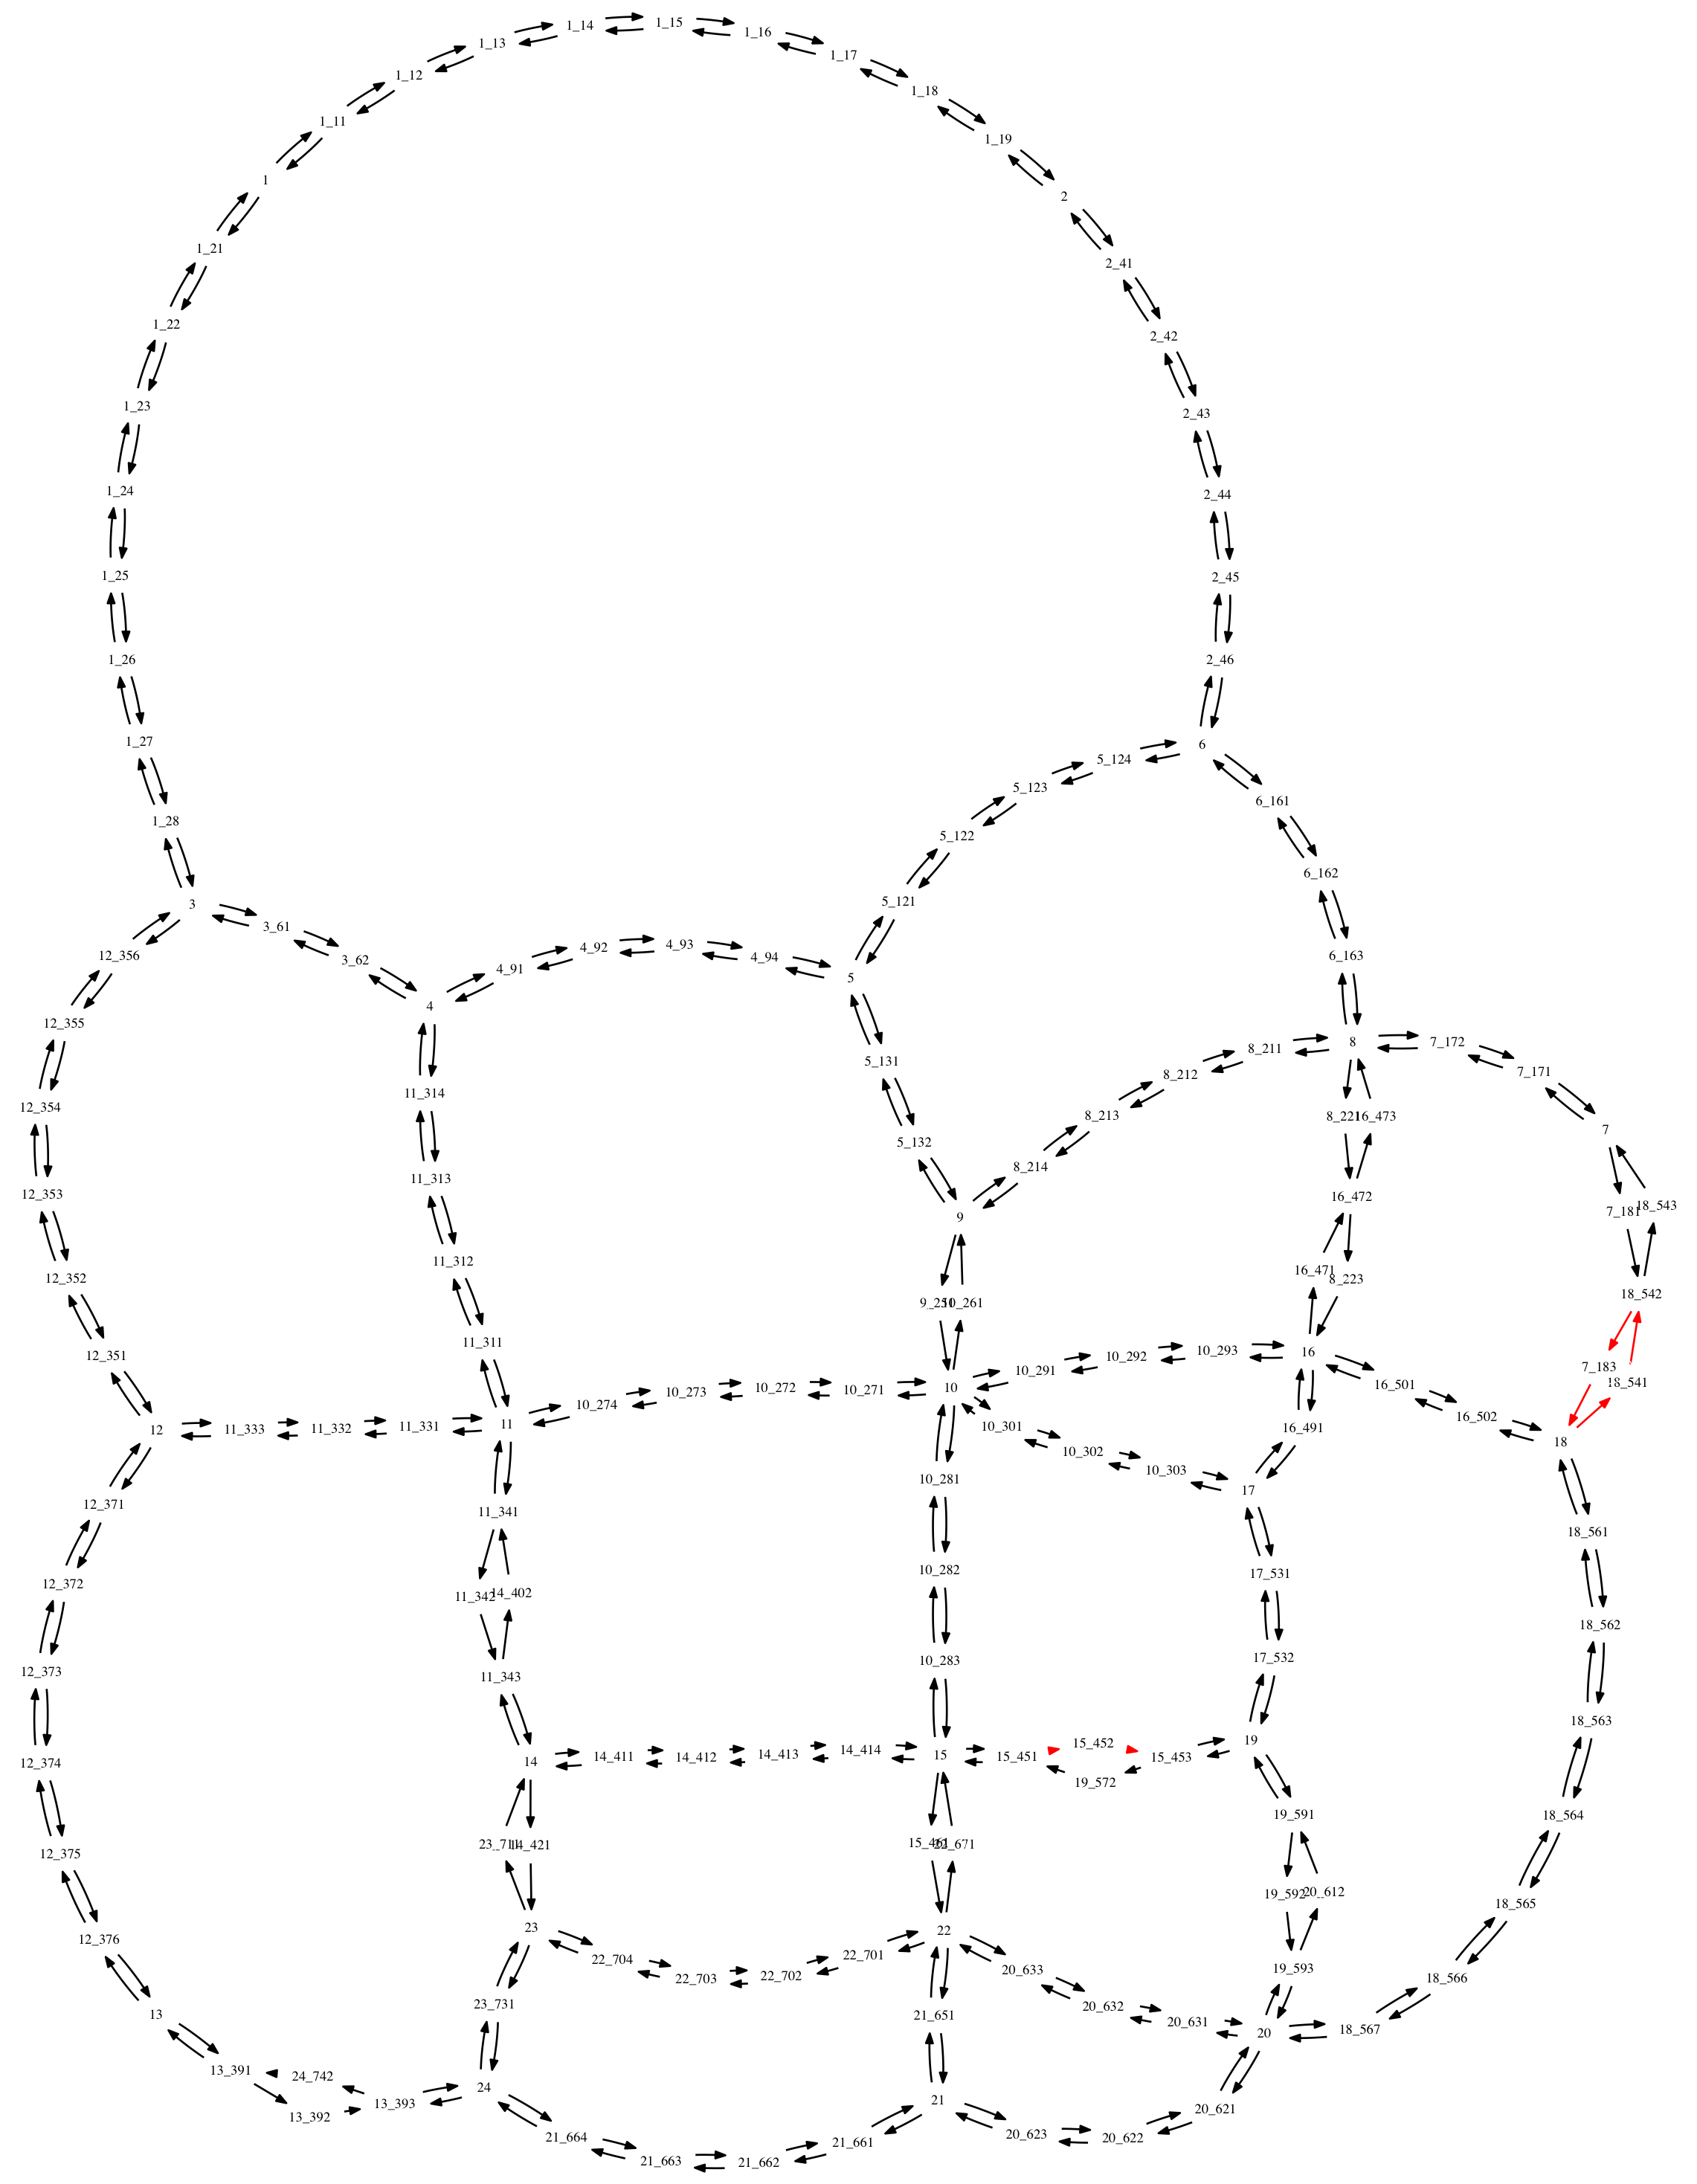
\includegraphics[totalheight=0.580\textheight, angle=90]{img/sioux-out/5/network2}
\caption{Sieć miasta Sioux Falls, rozwiązanie nr. 5.}
\label{sioux5}
\end{figure}

\begin{figure}[ht]
\centering
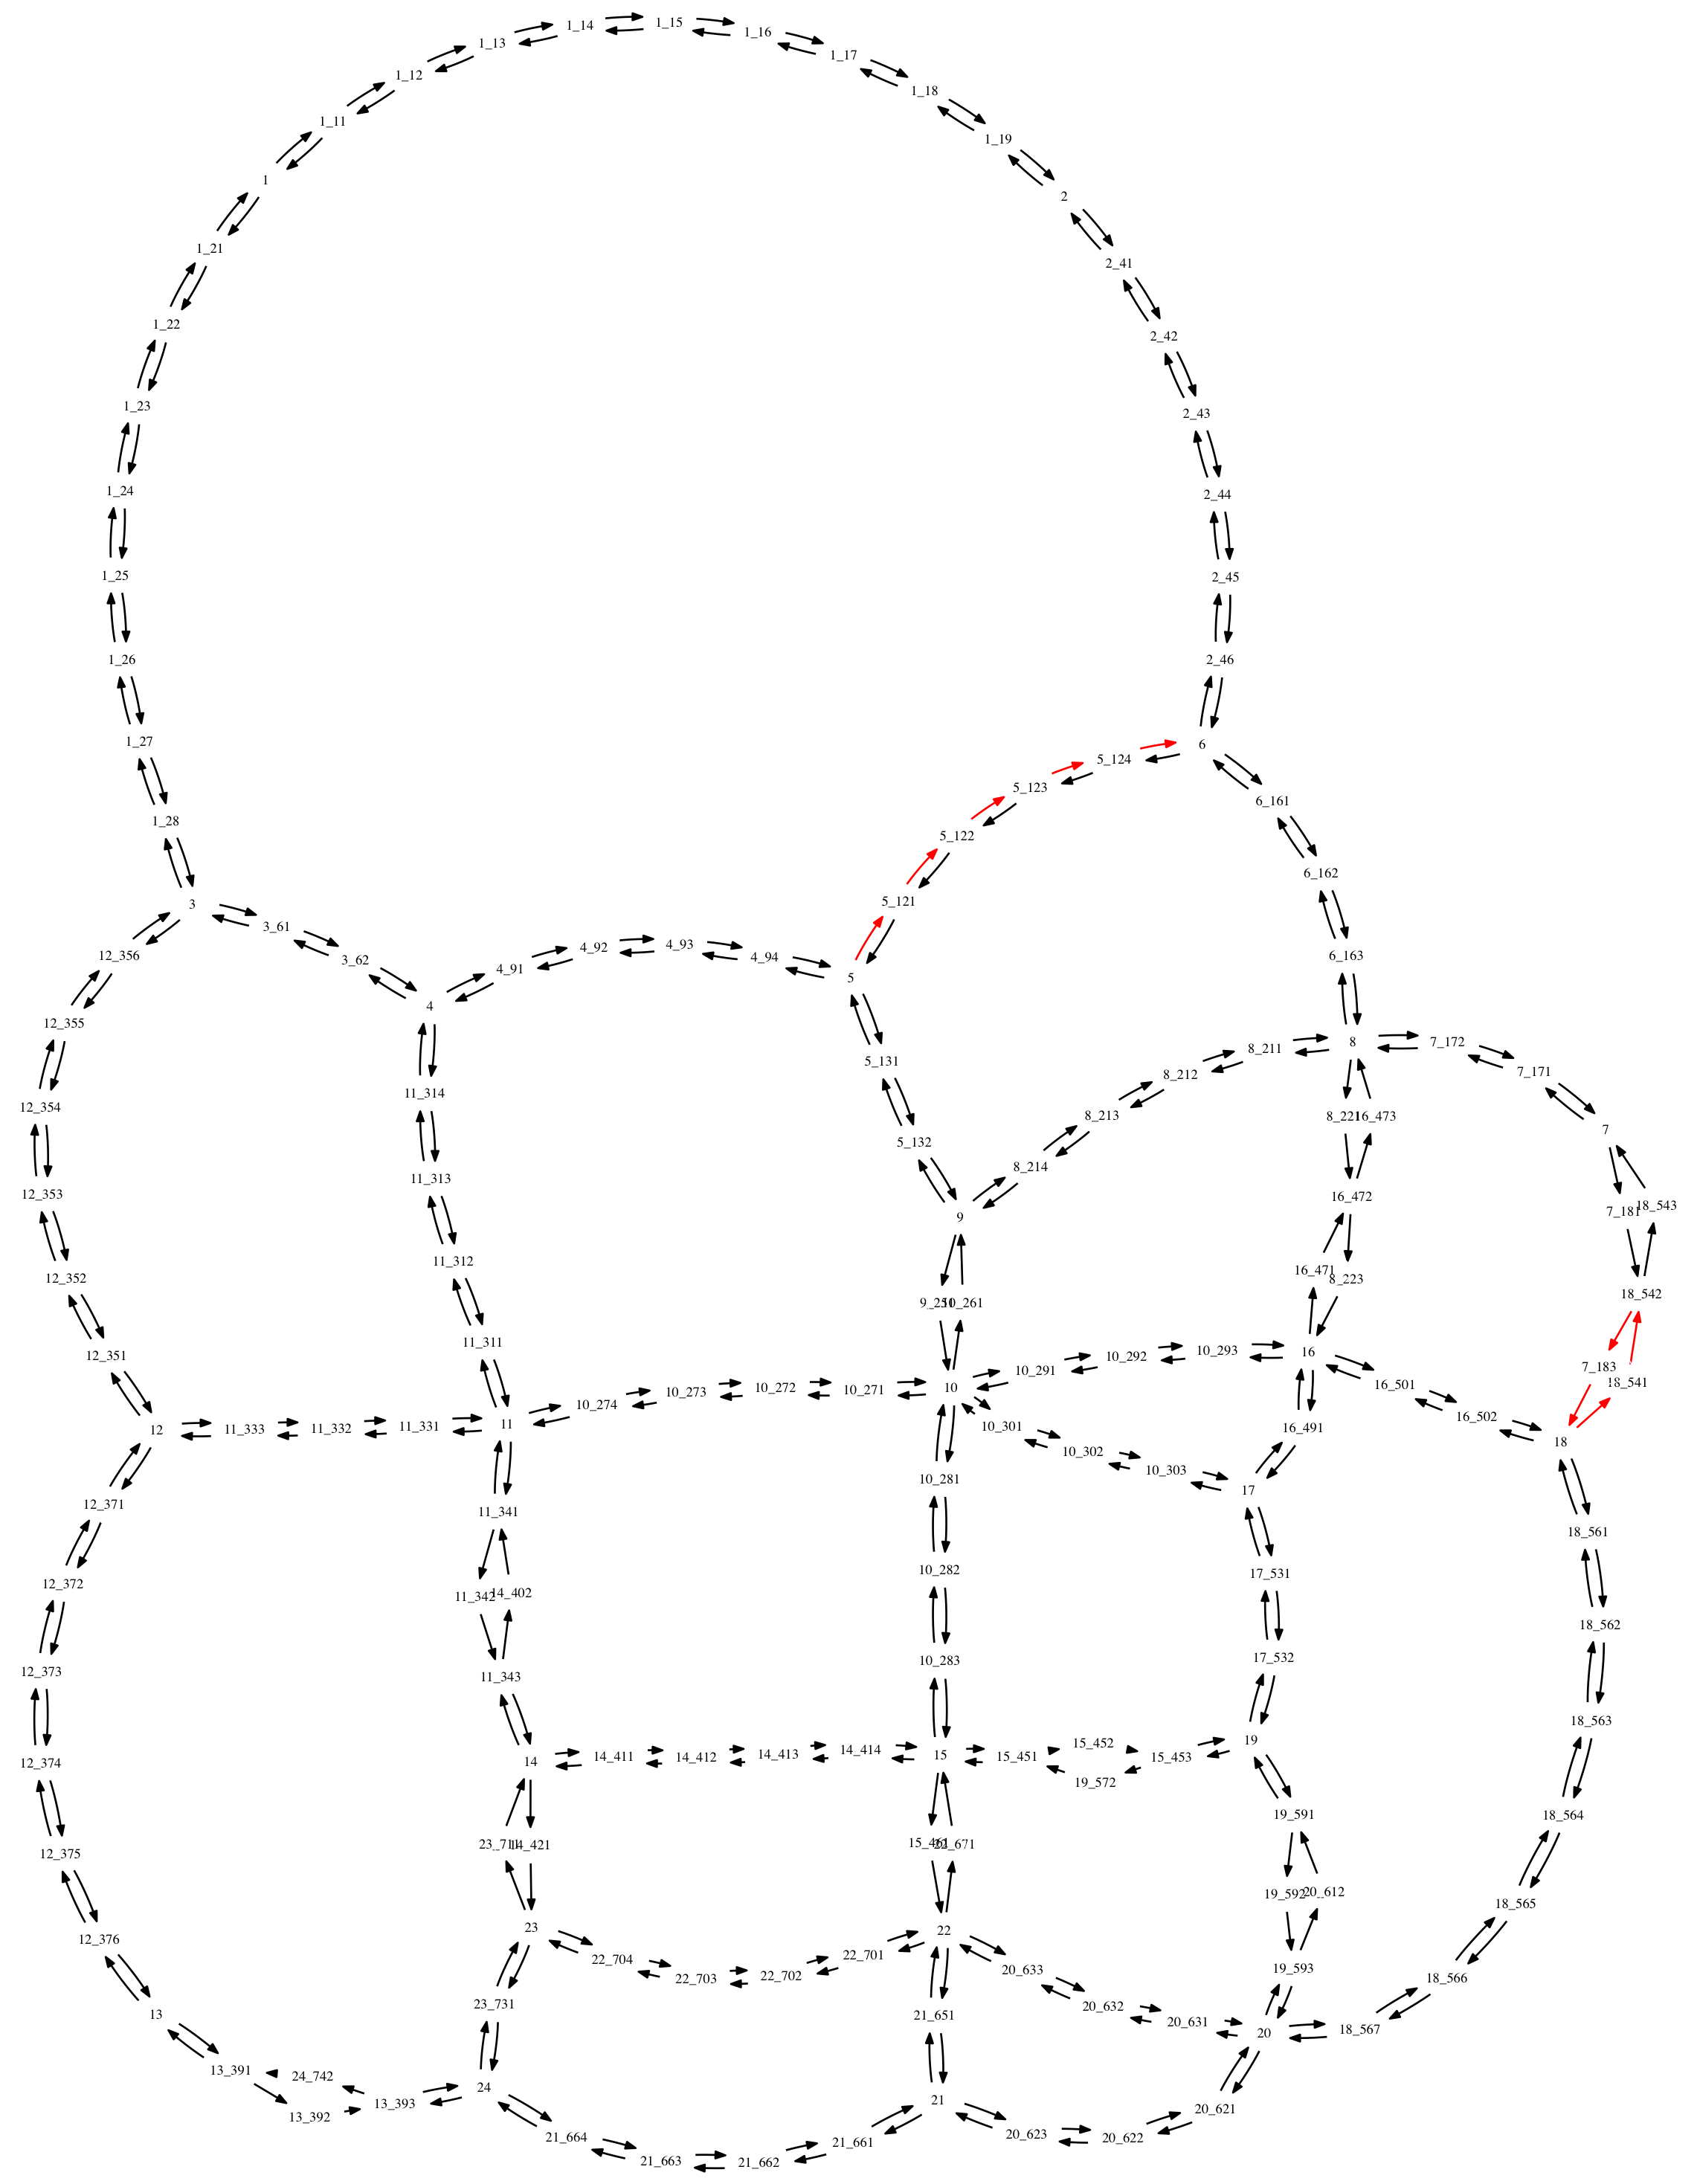
\includegraphics[totalheight=0.580\textheight, angle=90]{img/sioux-out/6/network2}
\caption{Sieć miasta Sioux Falls, rozwiązanie nr. 6.}
\label{sioux6}
\end{figure}

\begin{figure}[ht]
\centering
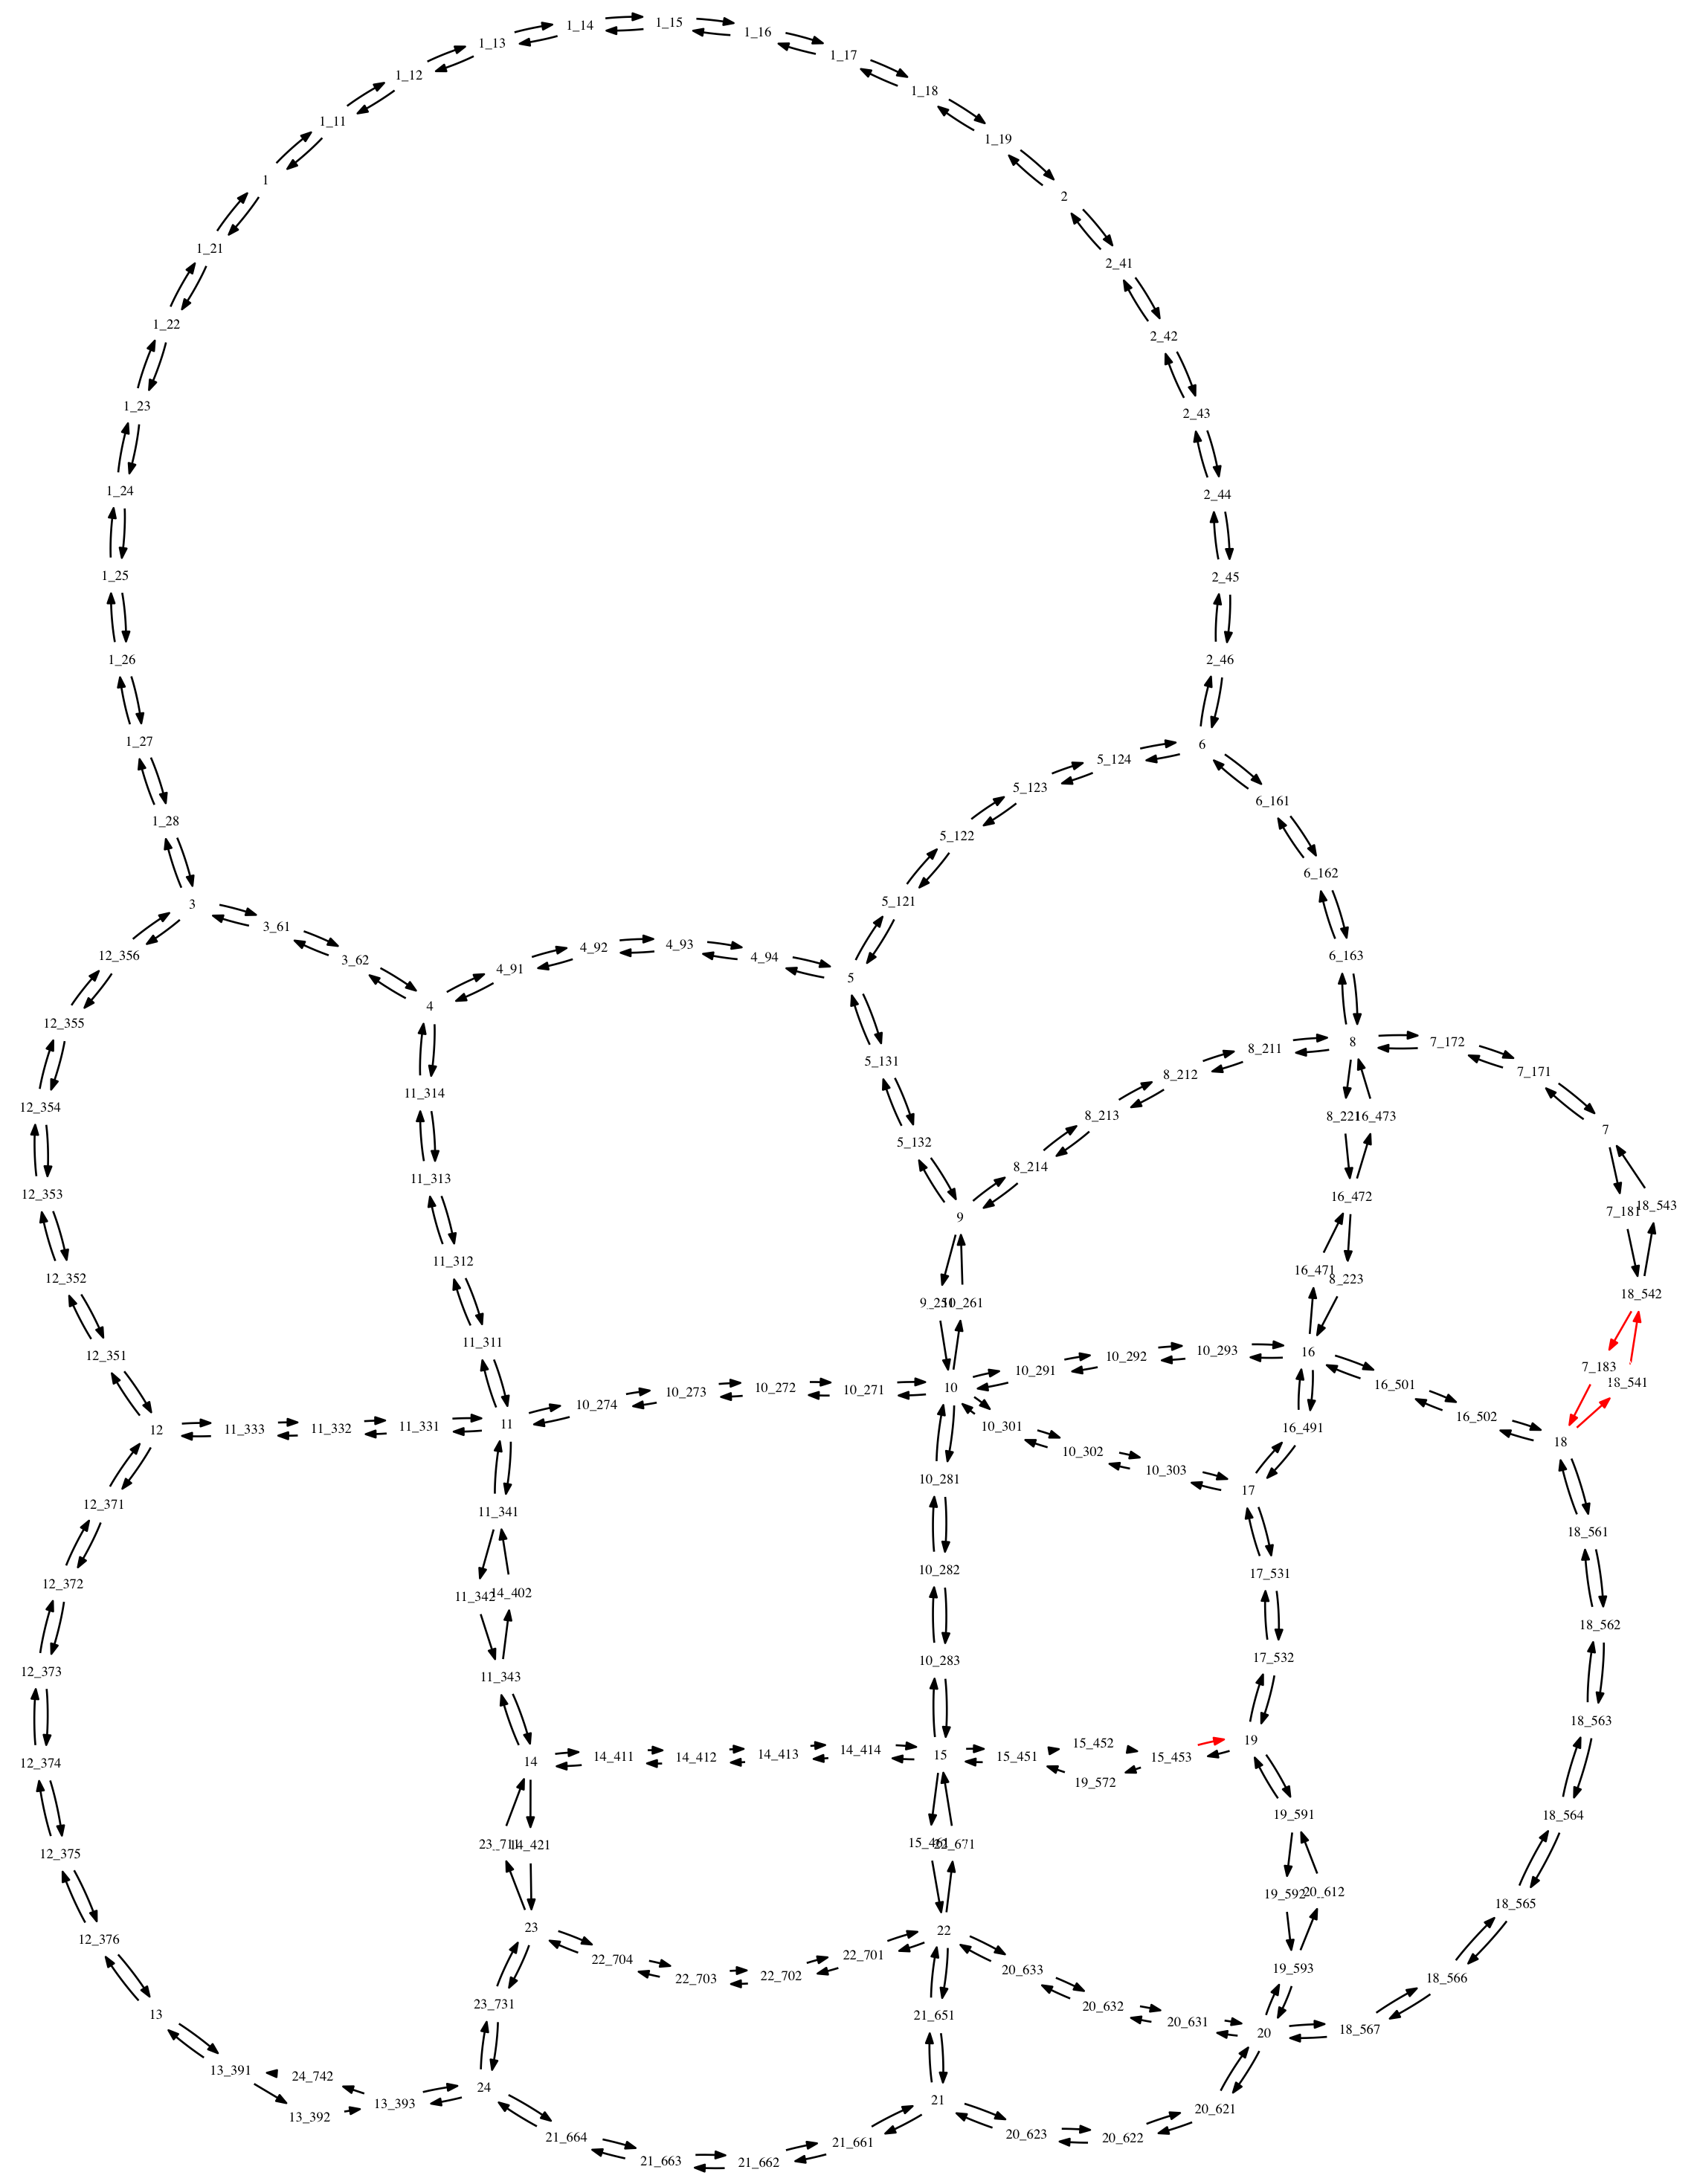
\includegraphics[totalheight=0.580\textheight, angle=90]{img/sioux-out/7/network2}
\caption{Sieć miasta Sioux Falls, rozwiązanie nr. 7.}
\label{sioux7}
\end{figure}

\begin{figure}[ht]
\centering
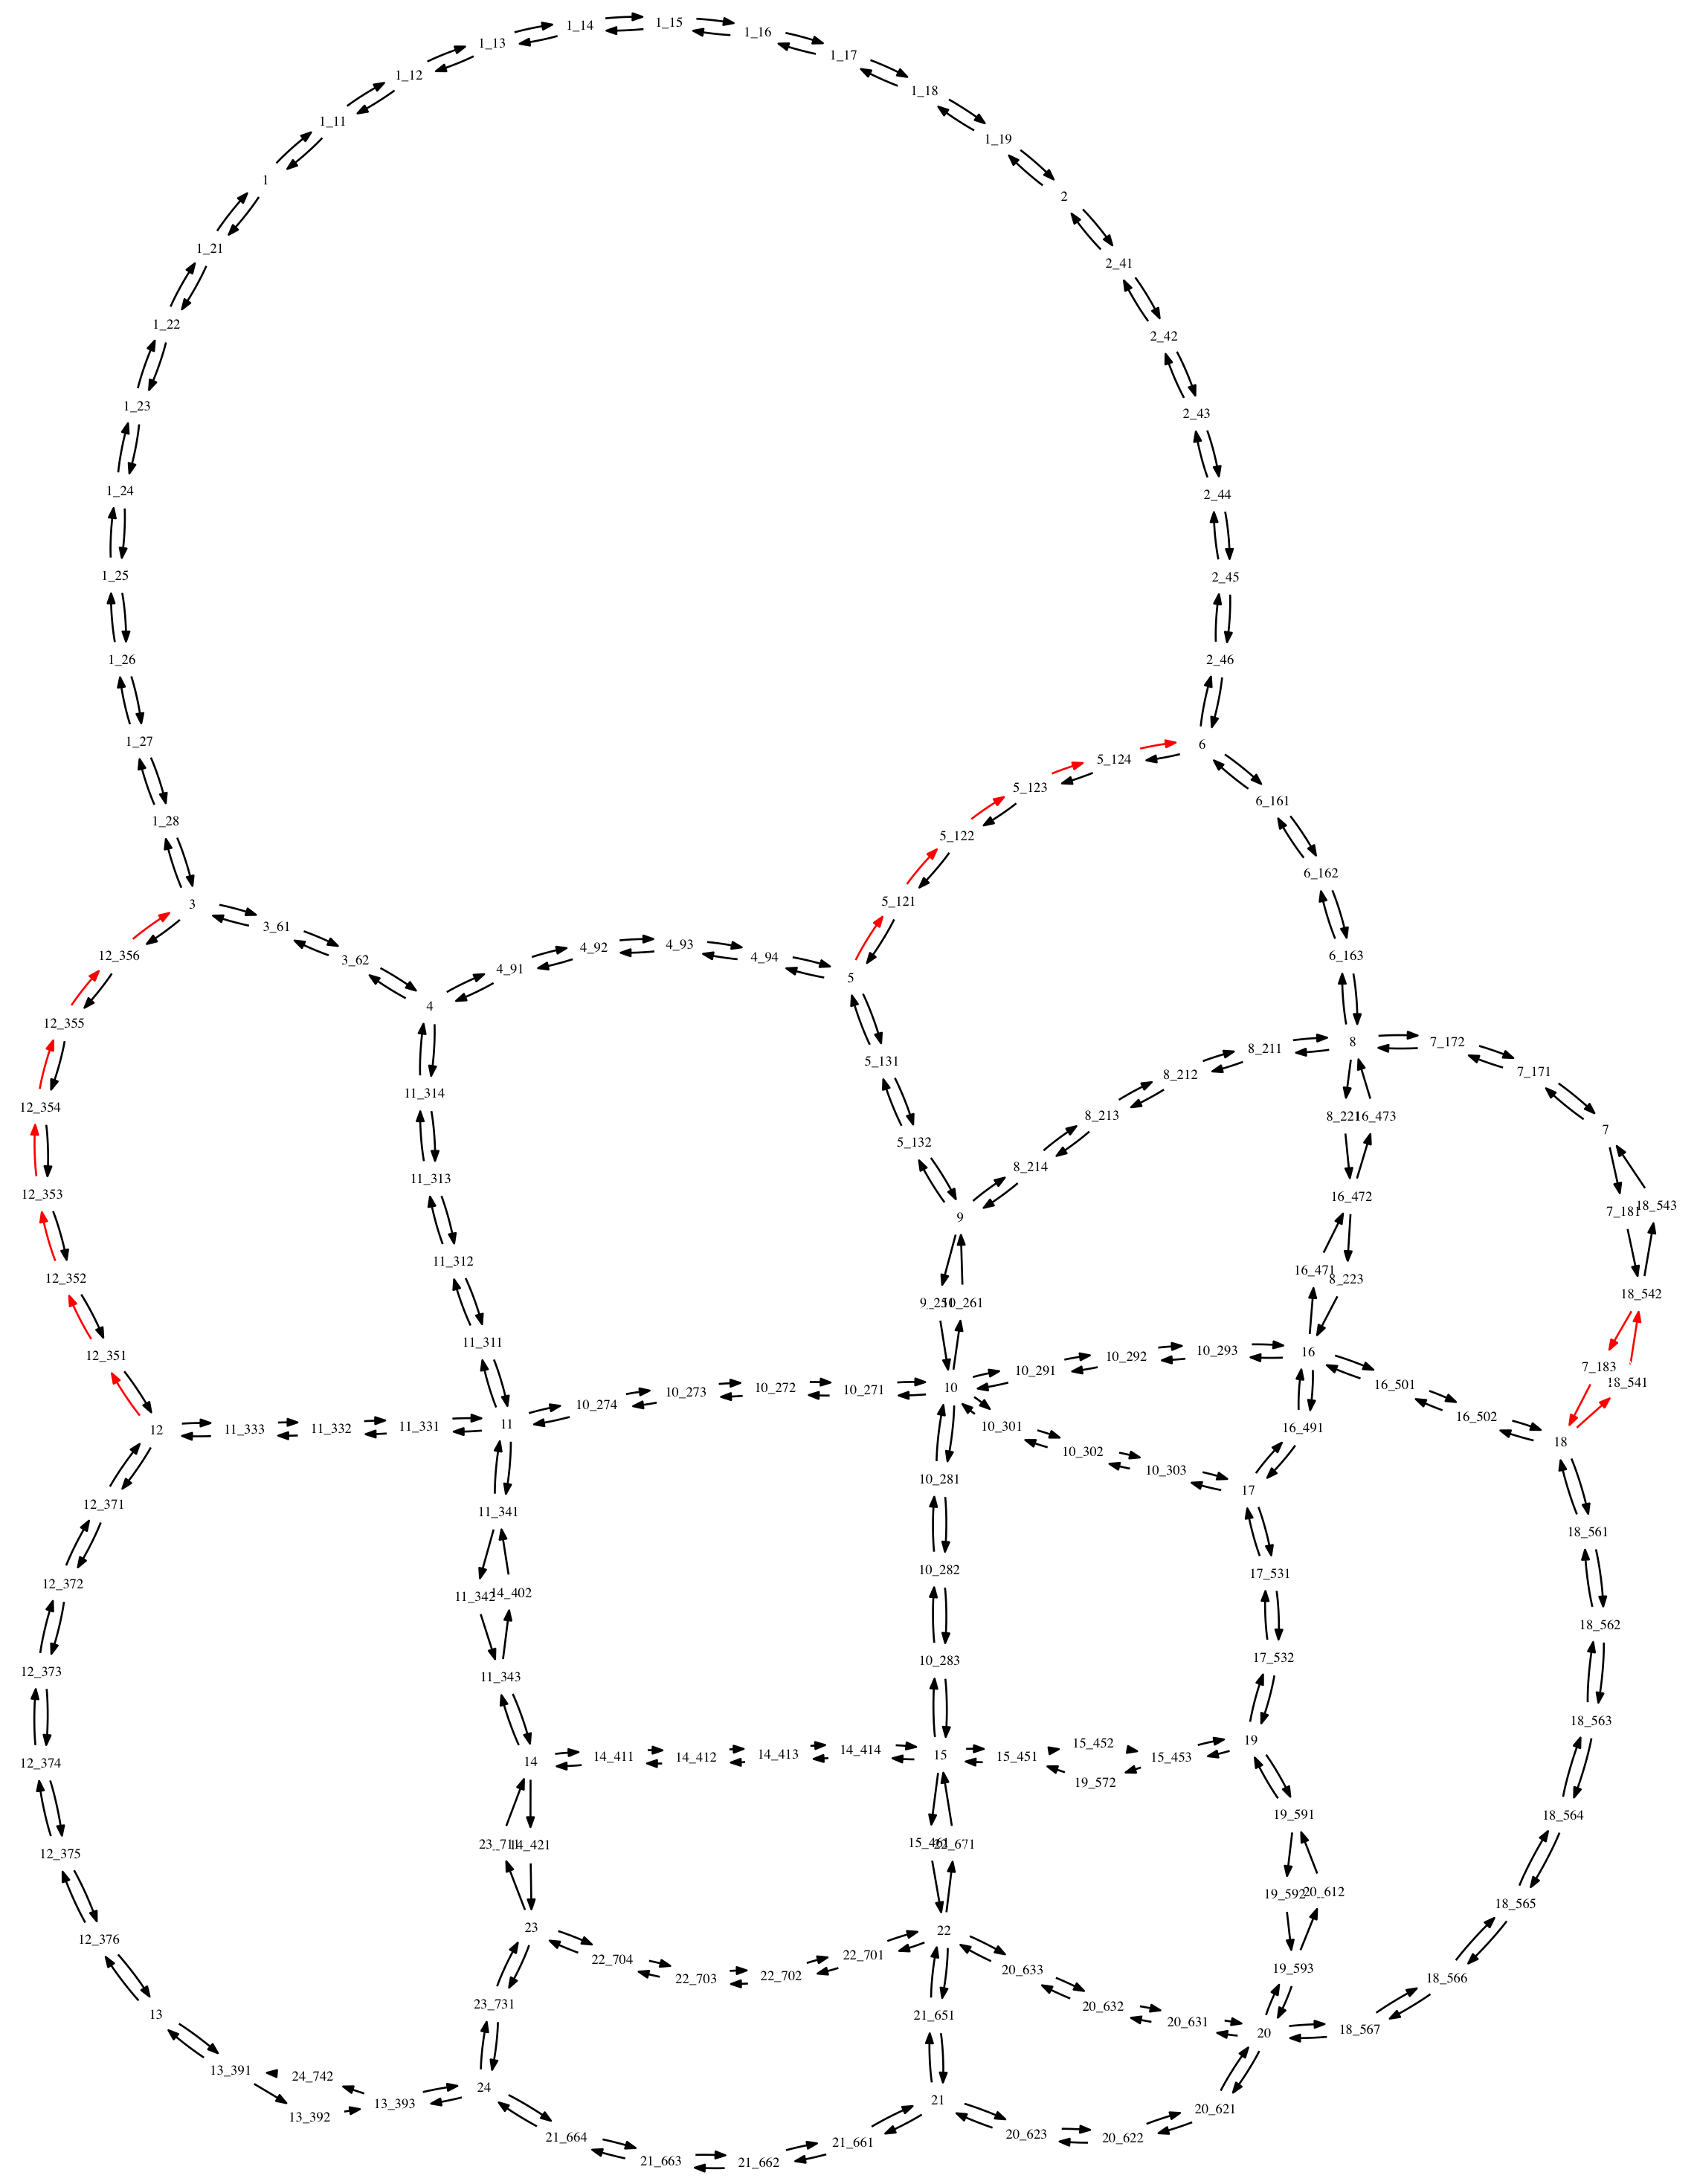
\includegraphics[totalheight=0.580\textheight, angle=90]{img/sioux-out/8/network2}
\caption{Sieć miasta Sioux Falls, rozwiązanie nr. 8.}
\label{sioux8}
\end{figure}

\begin{figure}[ht]
\centering
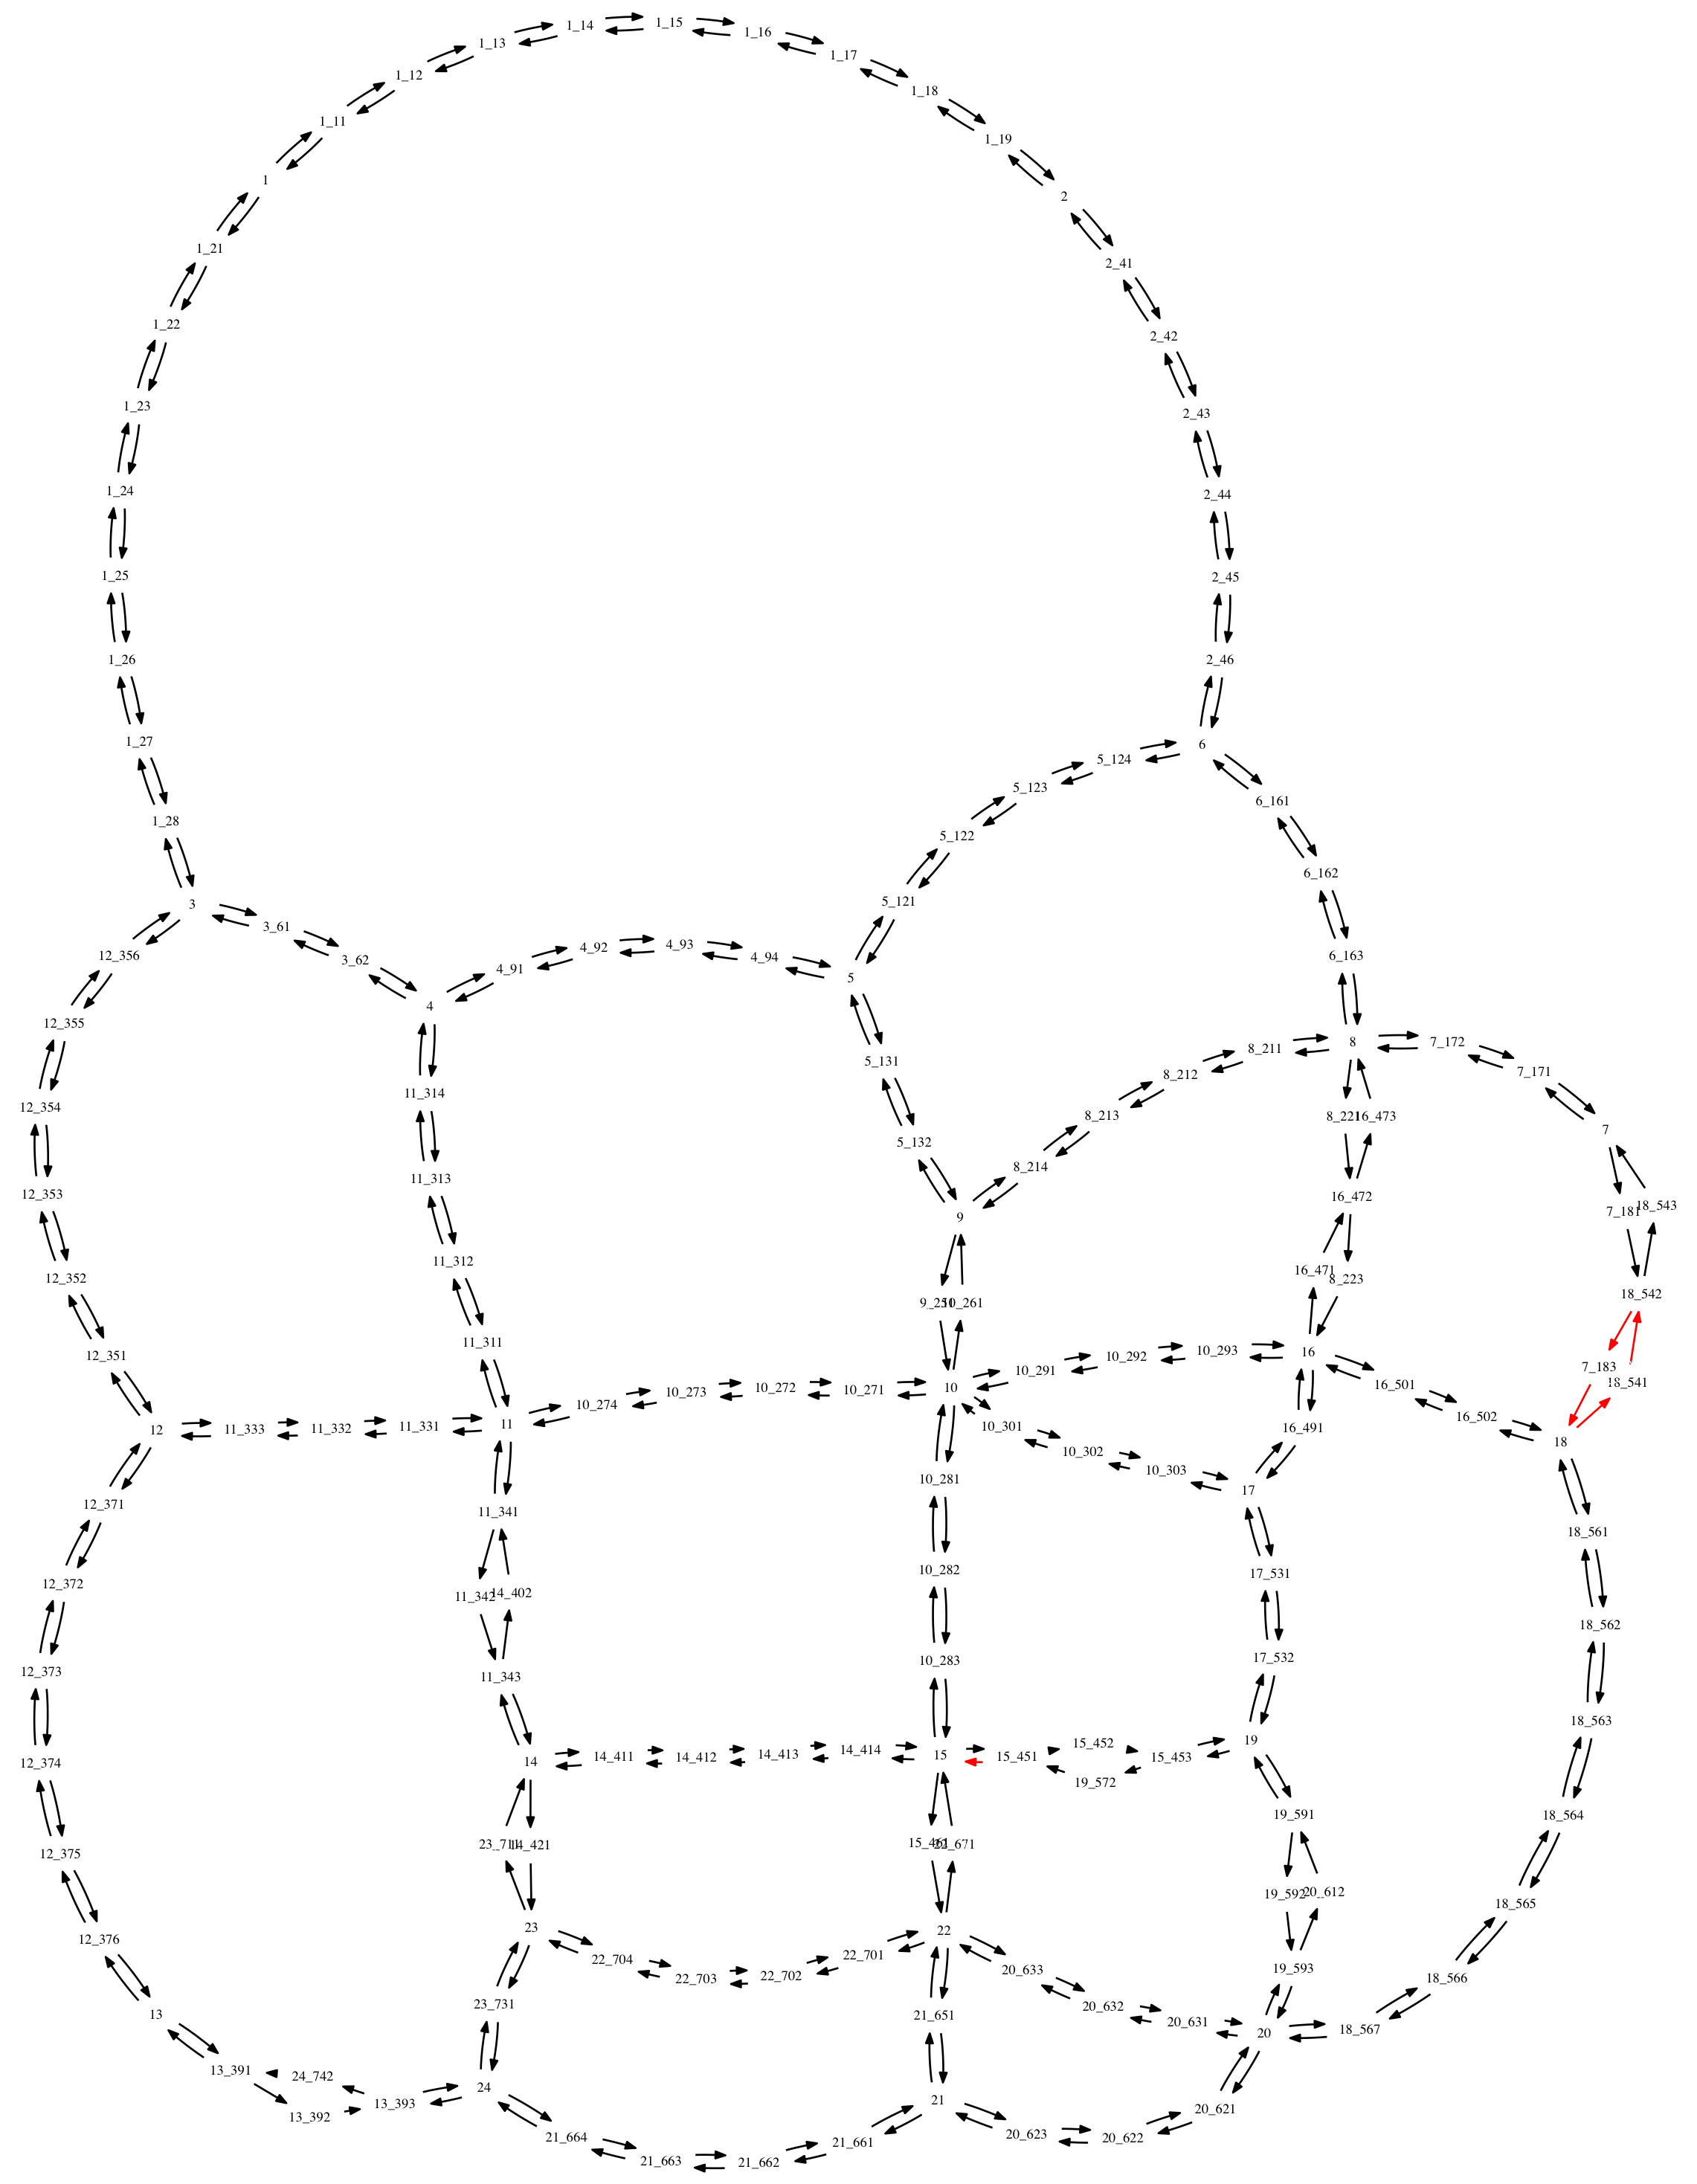
\includegraphics[totalheight=0.580\textheight, angle=90]{img/sioux-out/9/network2}
\caption{Sieć miasta Sioux Falls, rozwiązanie nr. 9.}
\label{sioux9}
\end{figure}

\begin{figure}[ht]
\centering
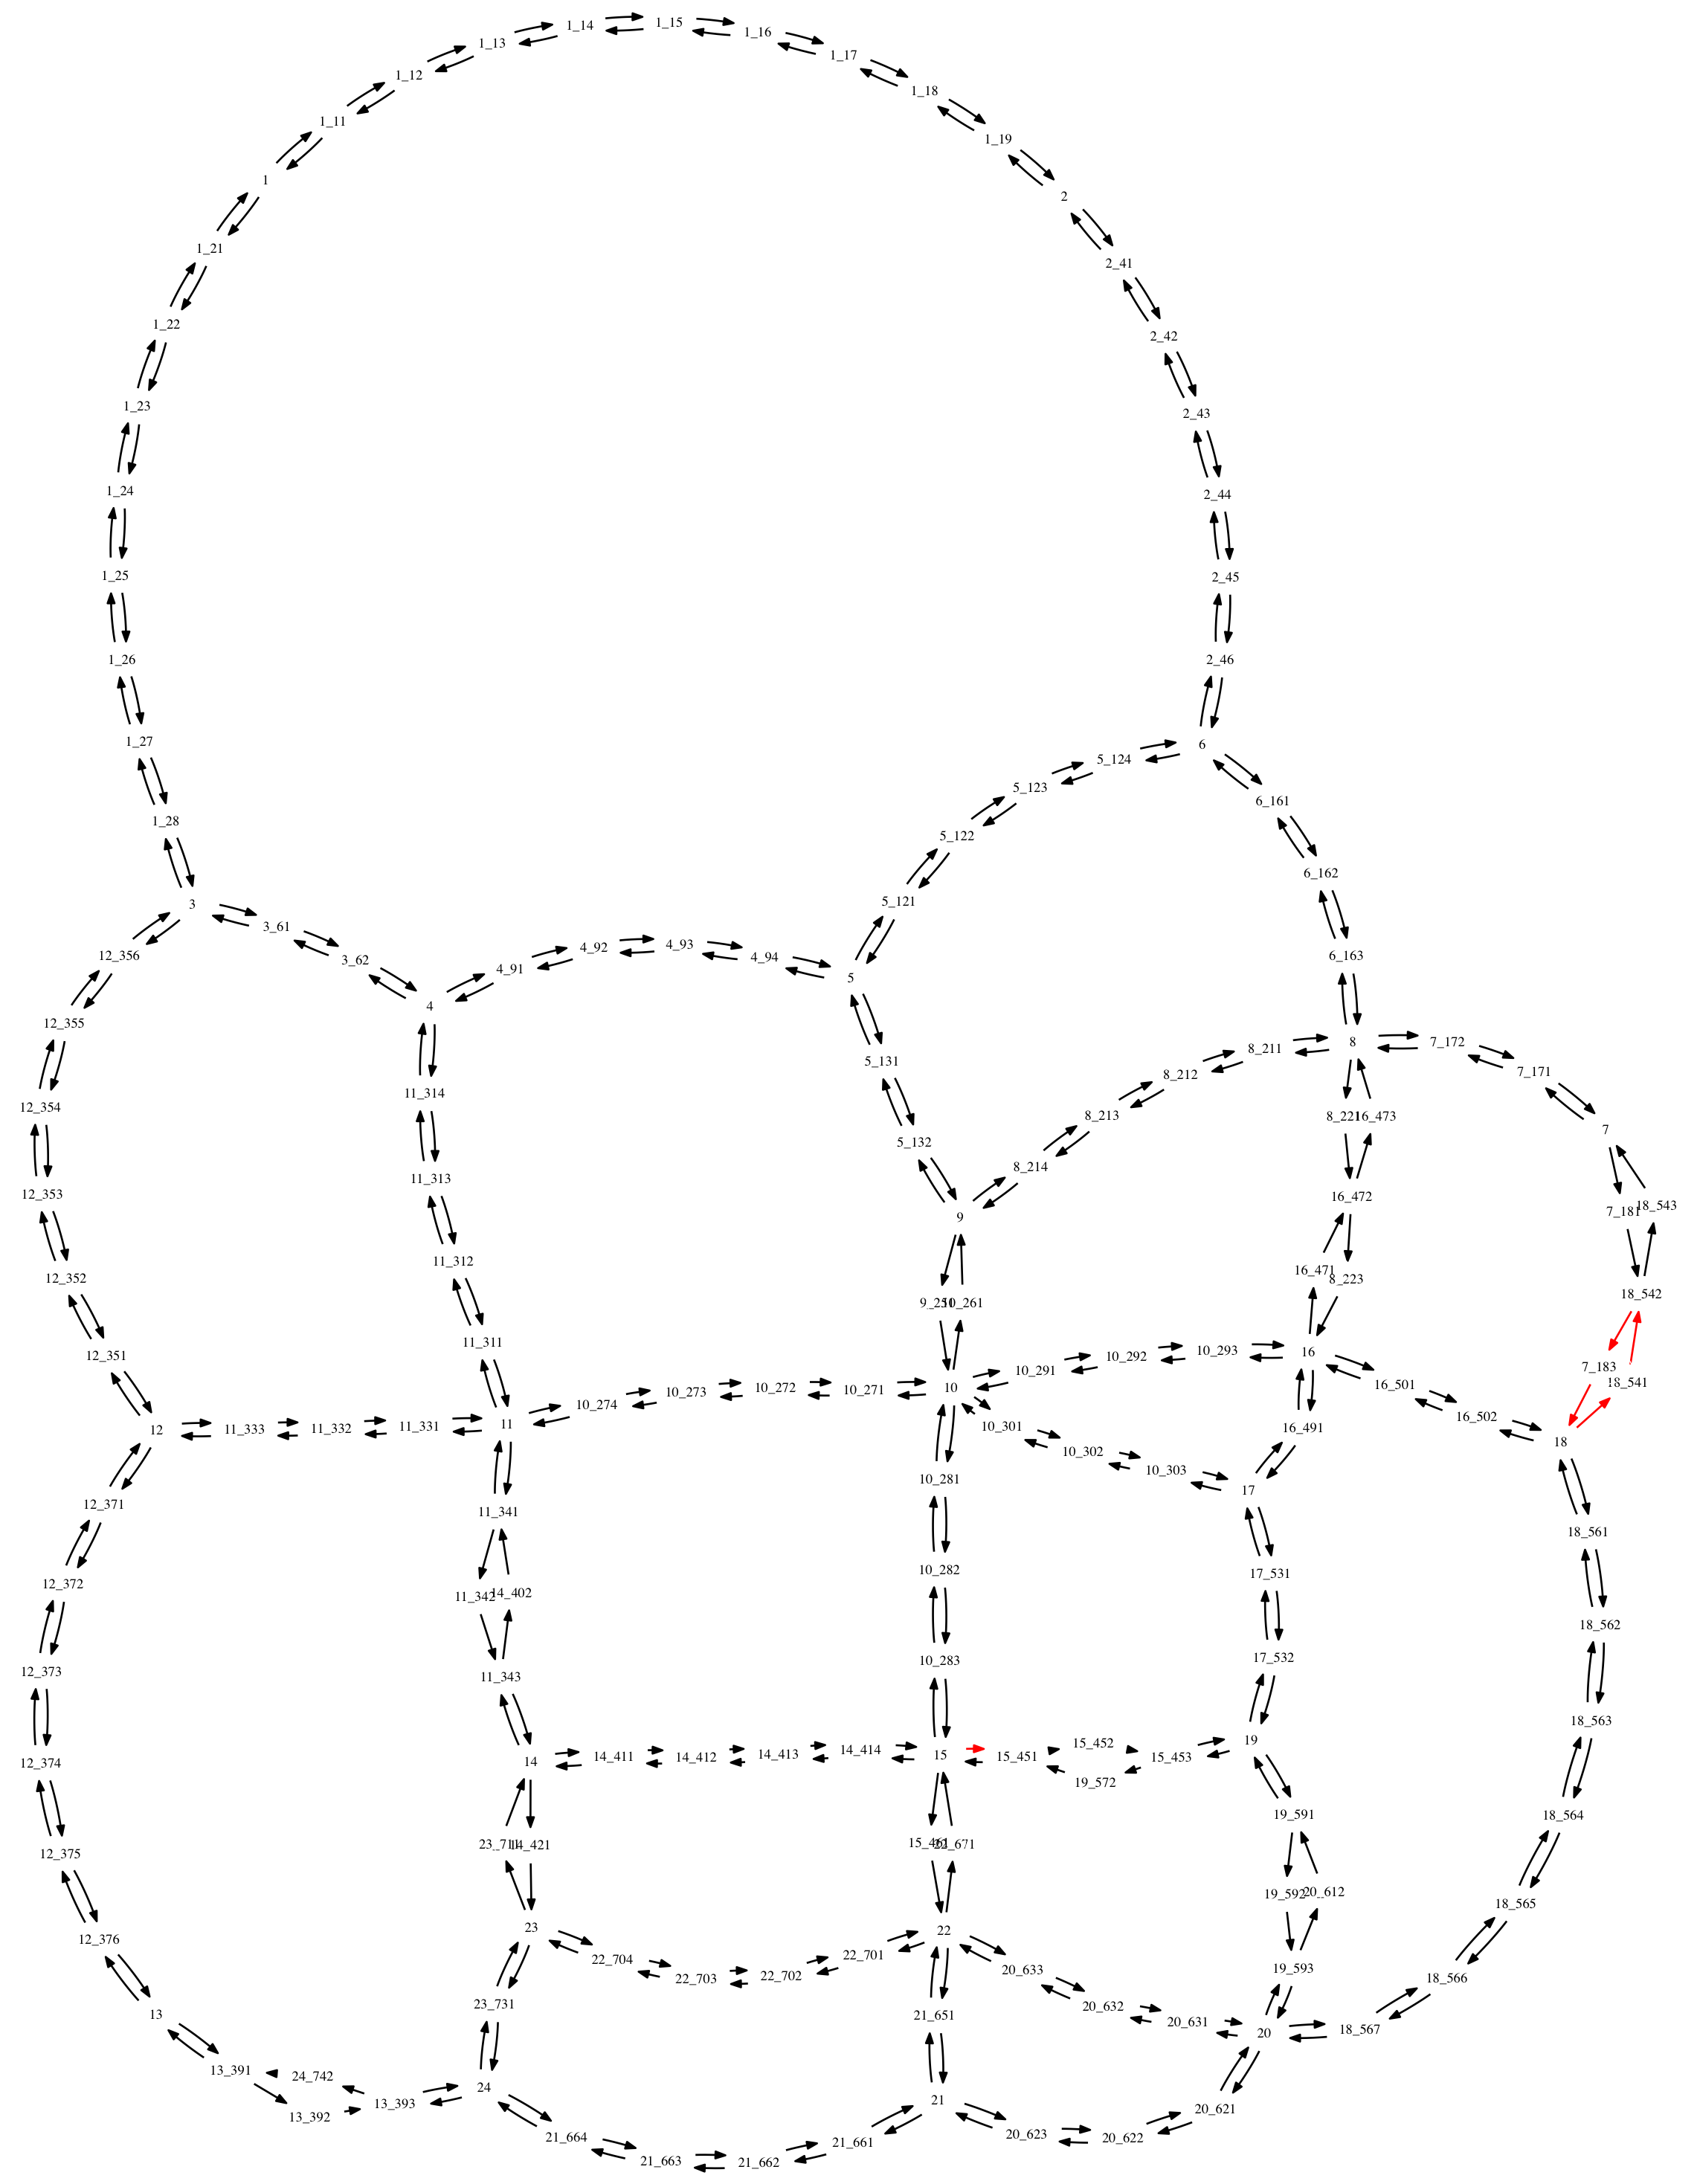
\includegraphics[totalheight=0.580\textheight, angle=90]{img/sioux-out/10/network2}
\caption{Sieć miasta Sioux Falls, rozwiązanie nr. 10.}
\label{sioux10}
\end{figure}

\begin{figure}[ht]
\centering
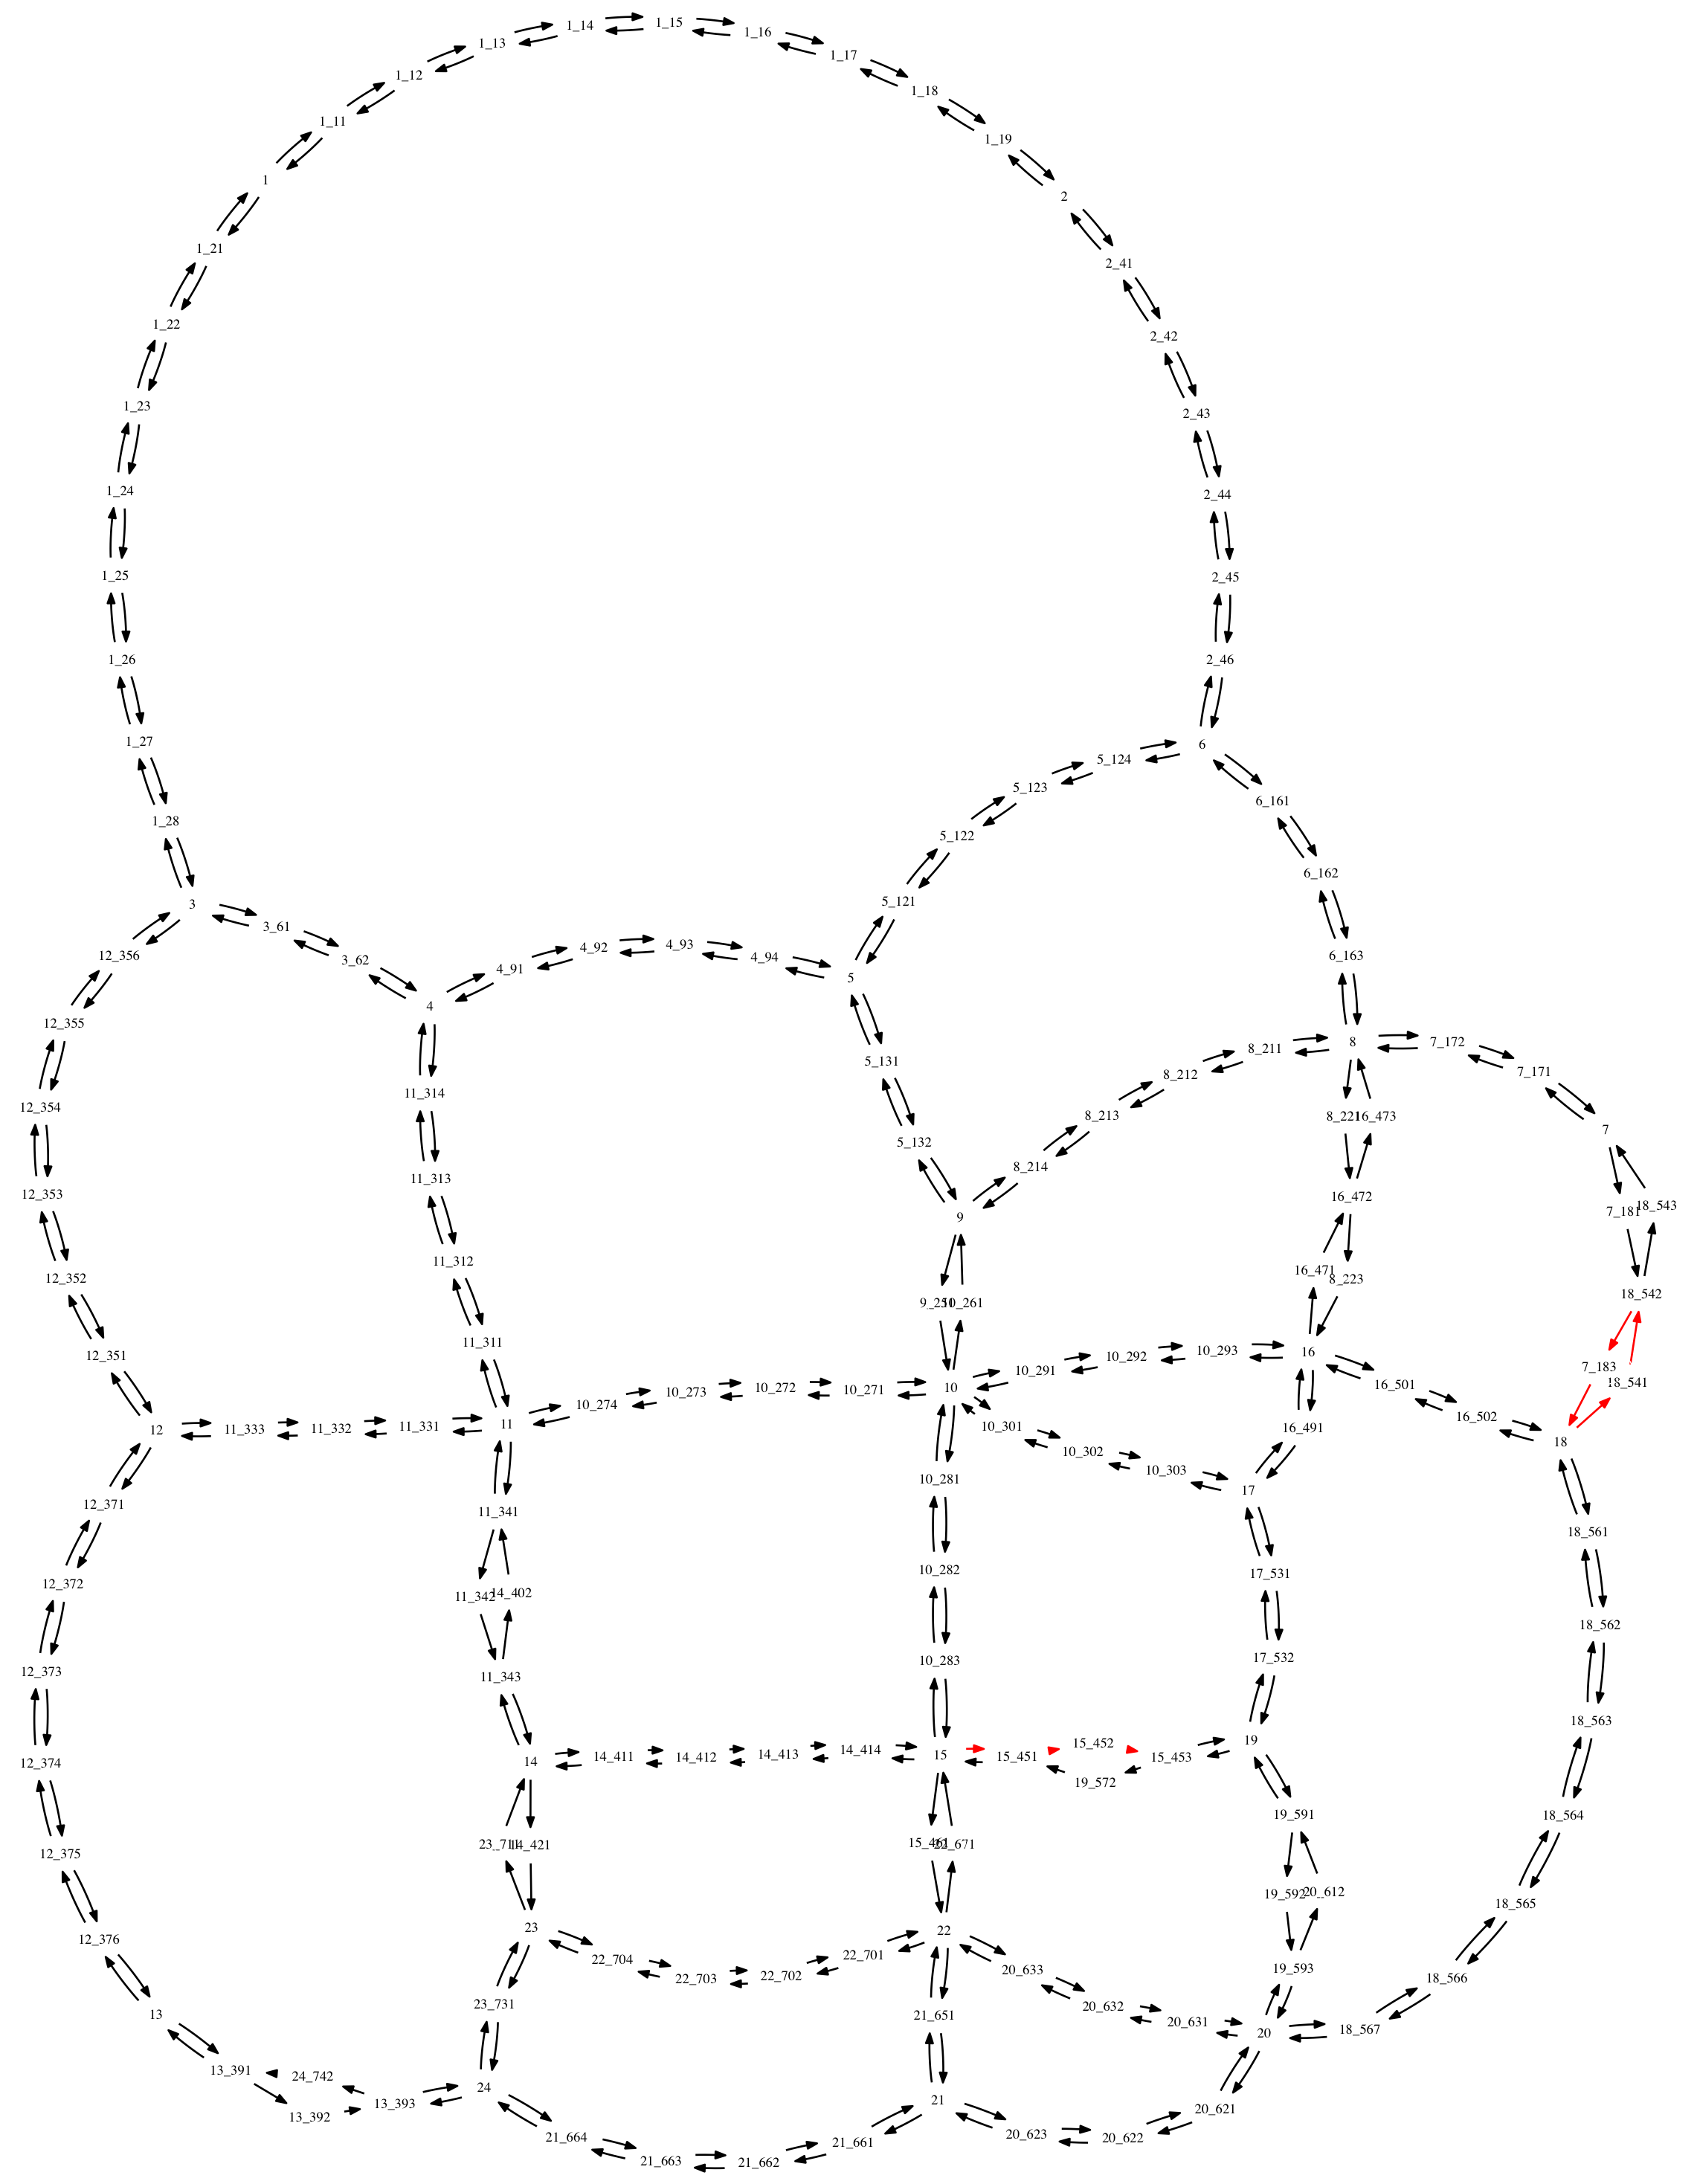
\includegraphics[totalheight=0.580\textheight, angle=90]{img/sioux-out/11/network2}
\caption{Sieć miasta Sioux Falls, rozwiązanie nr. 11.}
\label{sioux11}
\end{figure}

\begin{figure}[ht]
\centering
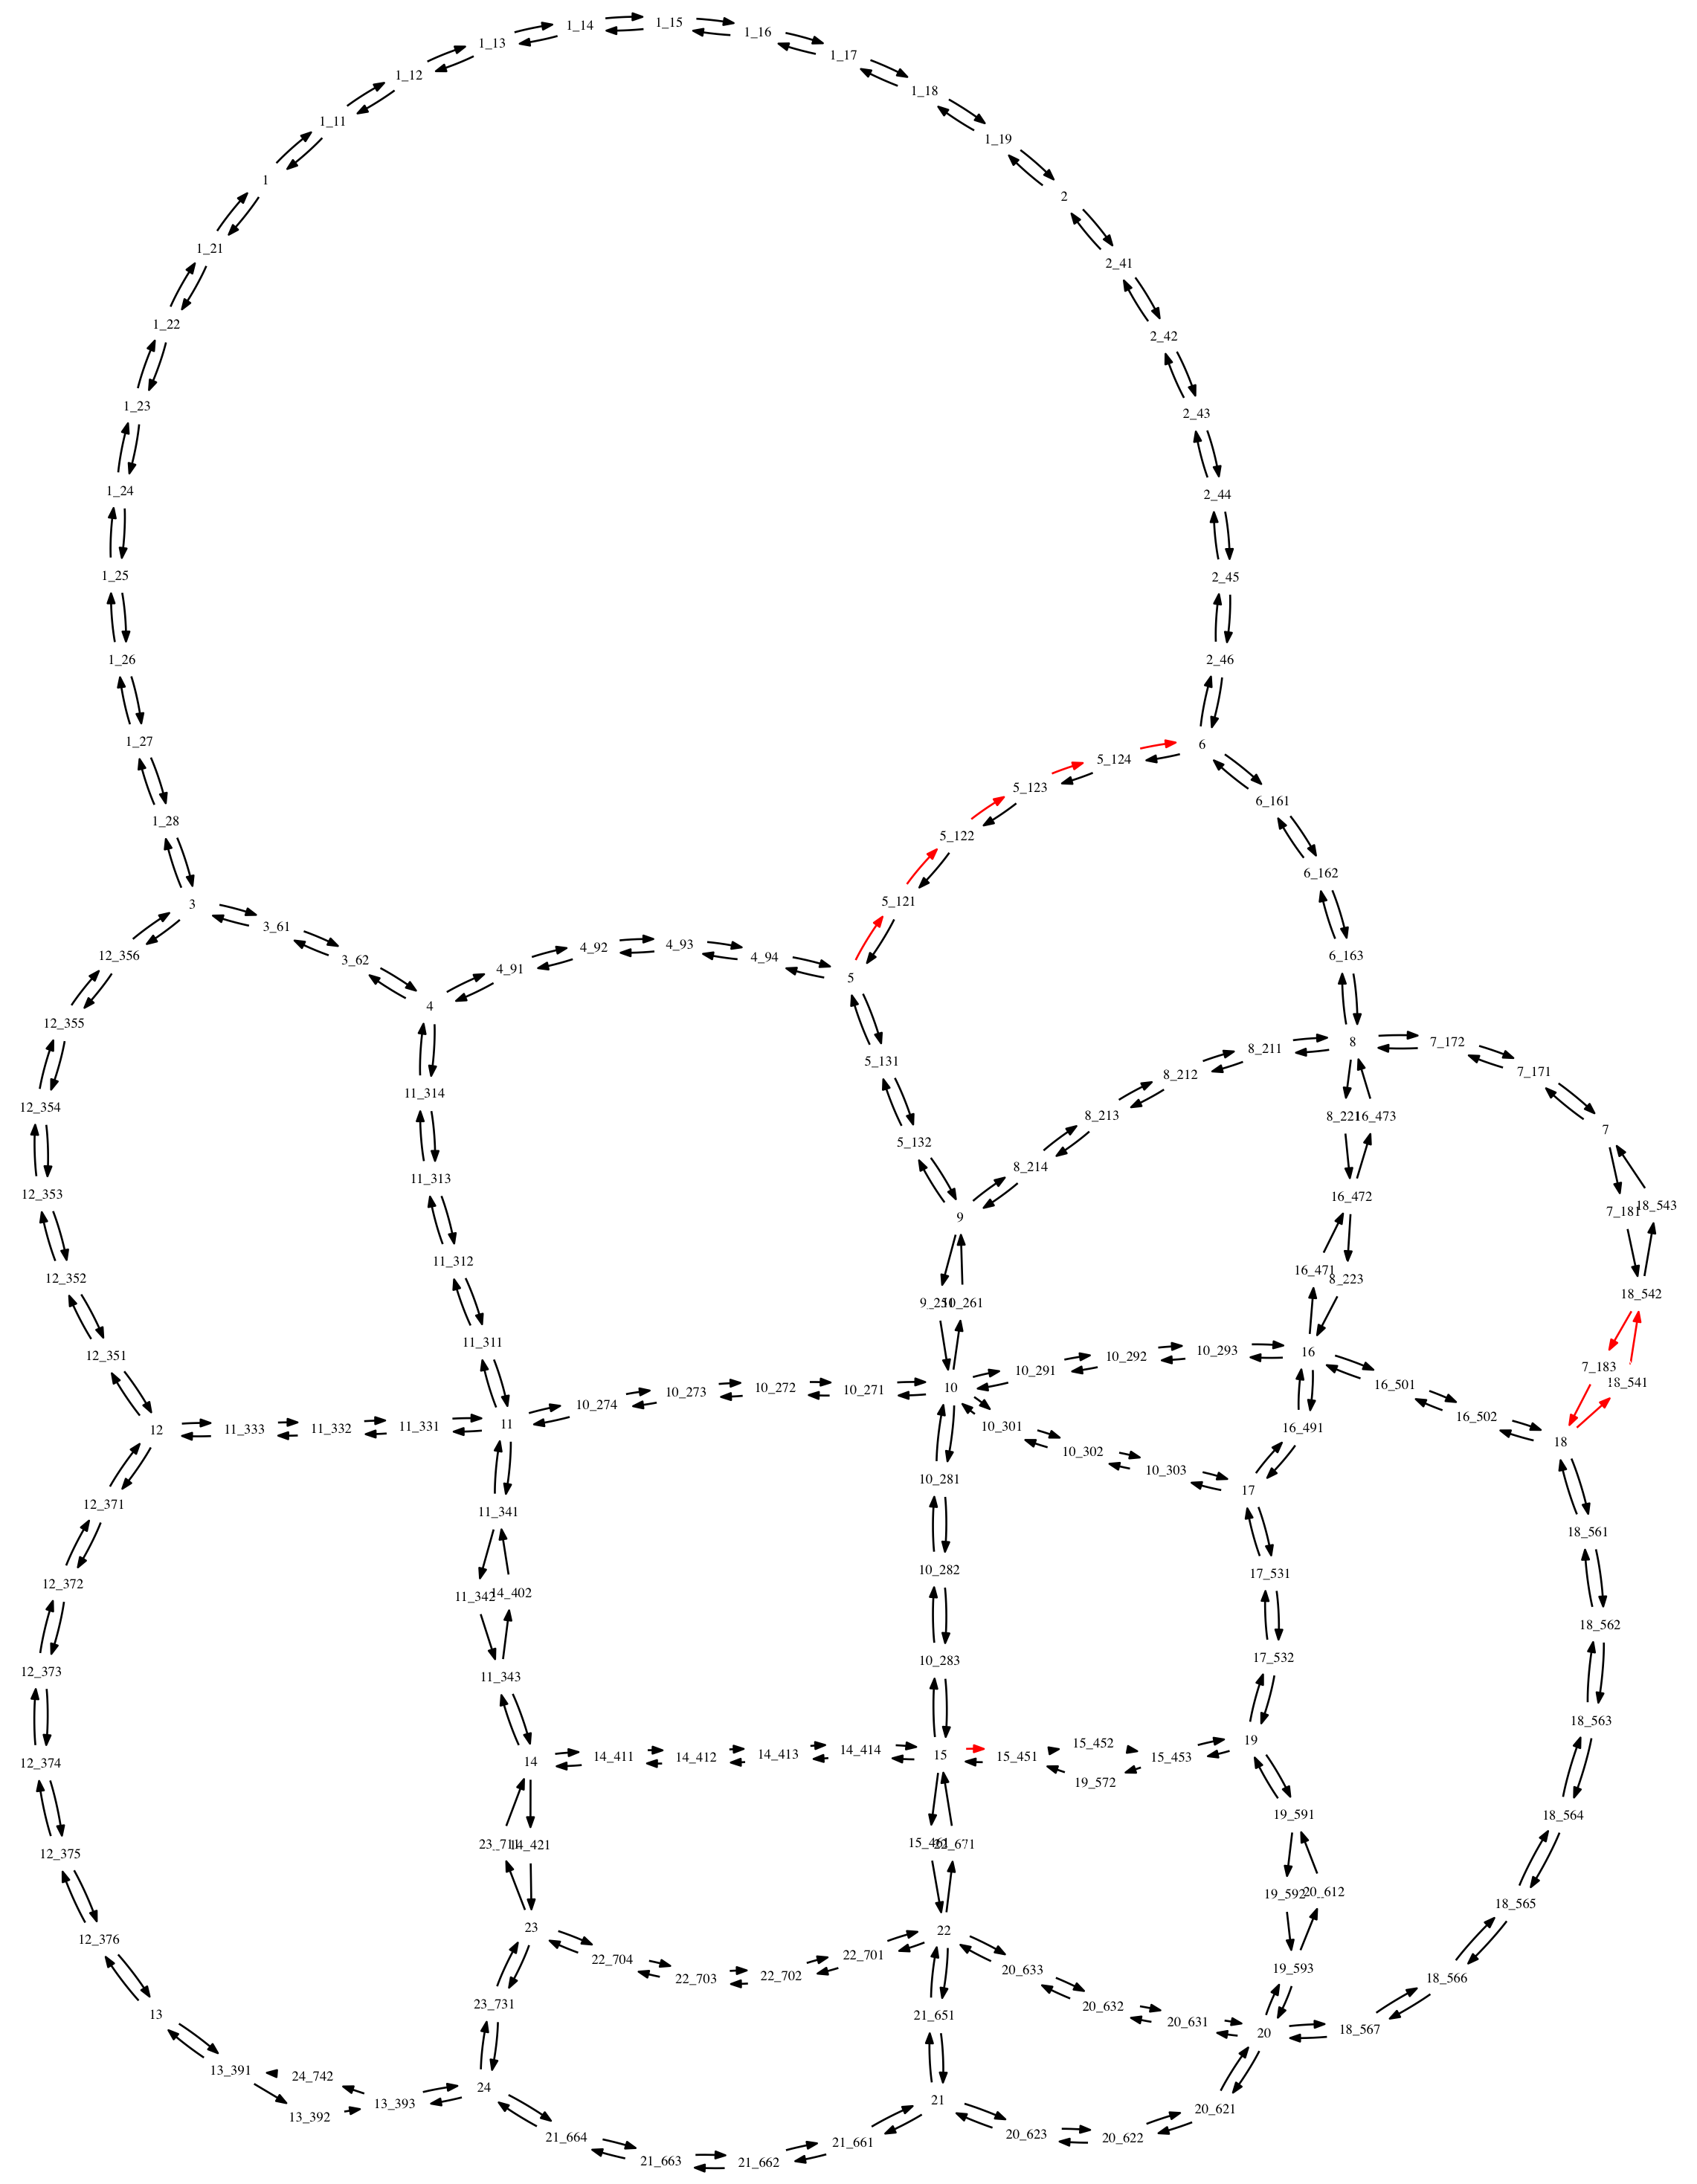
\includegraphics[totalheight=0.580\textheight, angle=90]{img/sioux-out/12/network2}
\caption{Sieć miasta Sioux Falls, rozwiązanie nr. 12.}
\label{sioux12}
\end{figure}

\begin{figure}[ht]
\centering
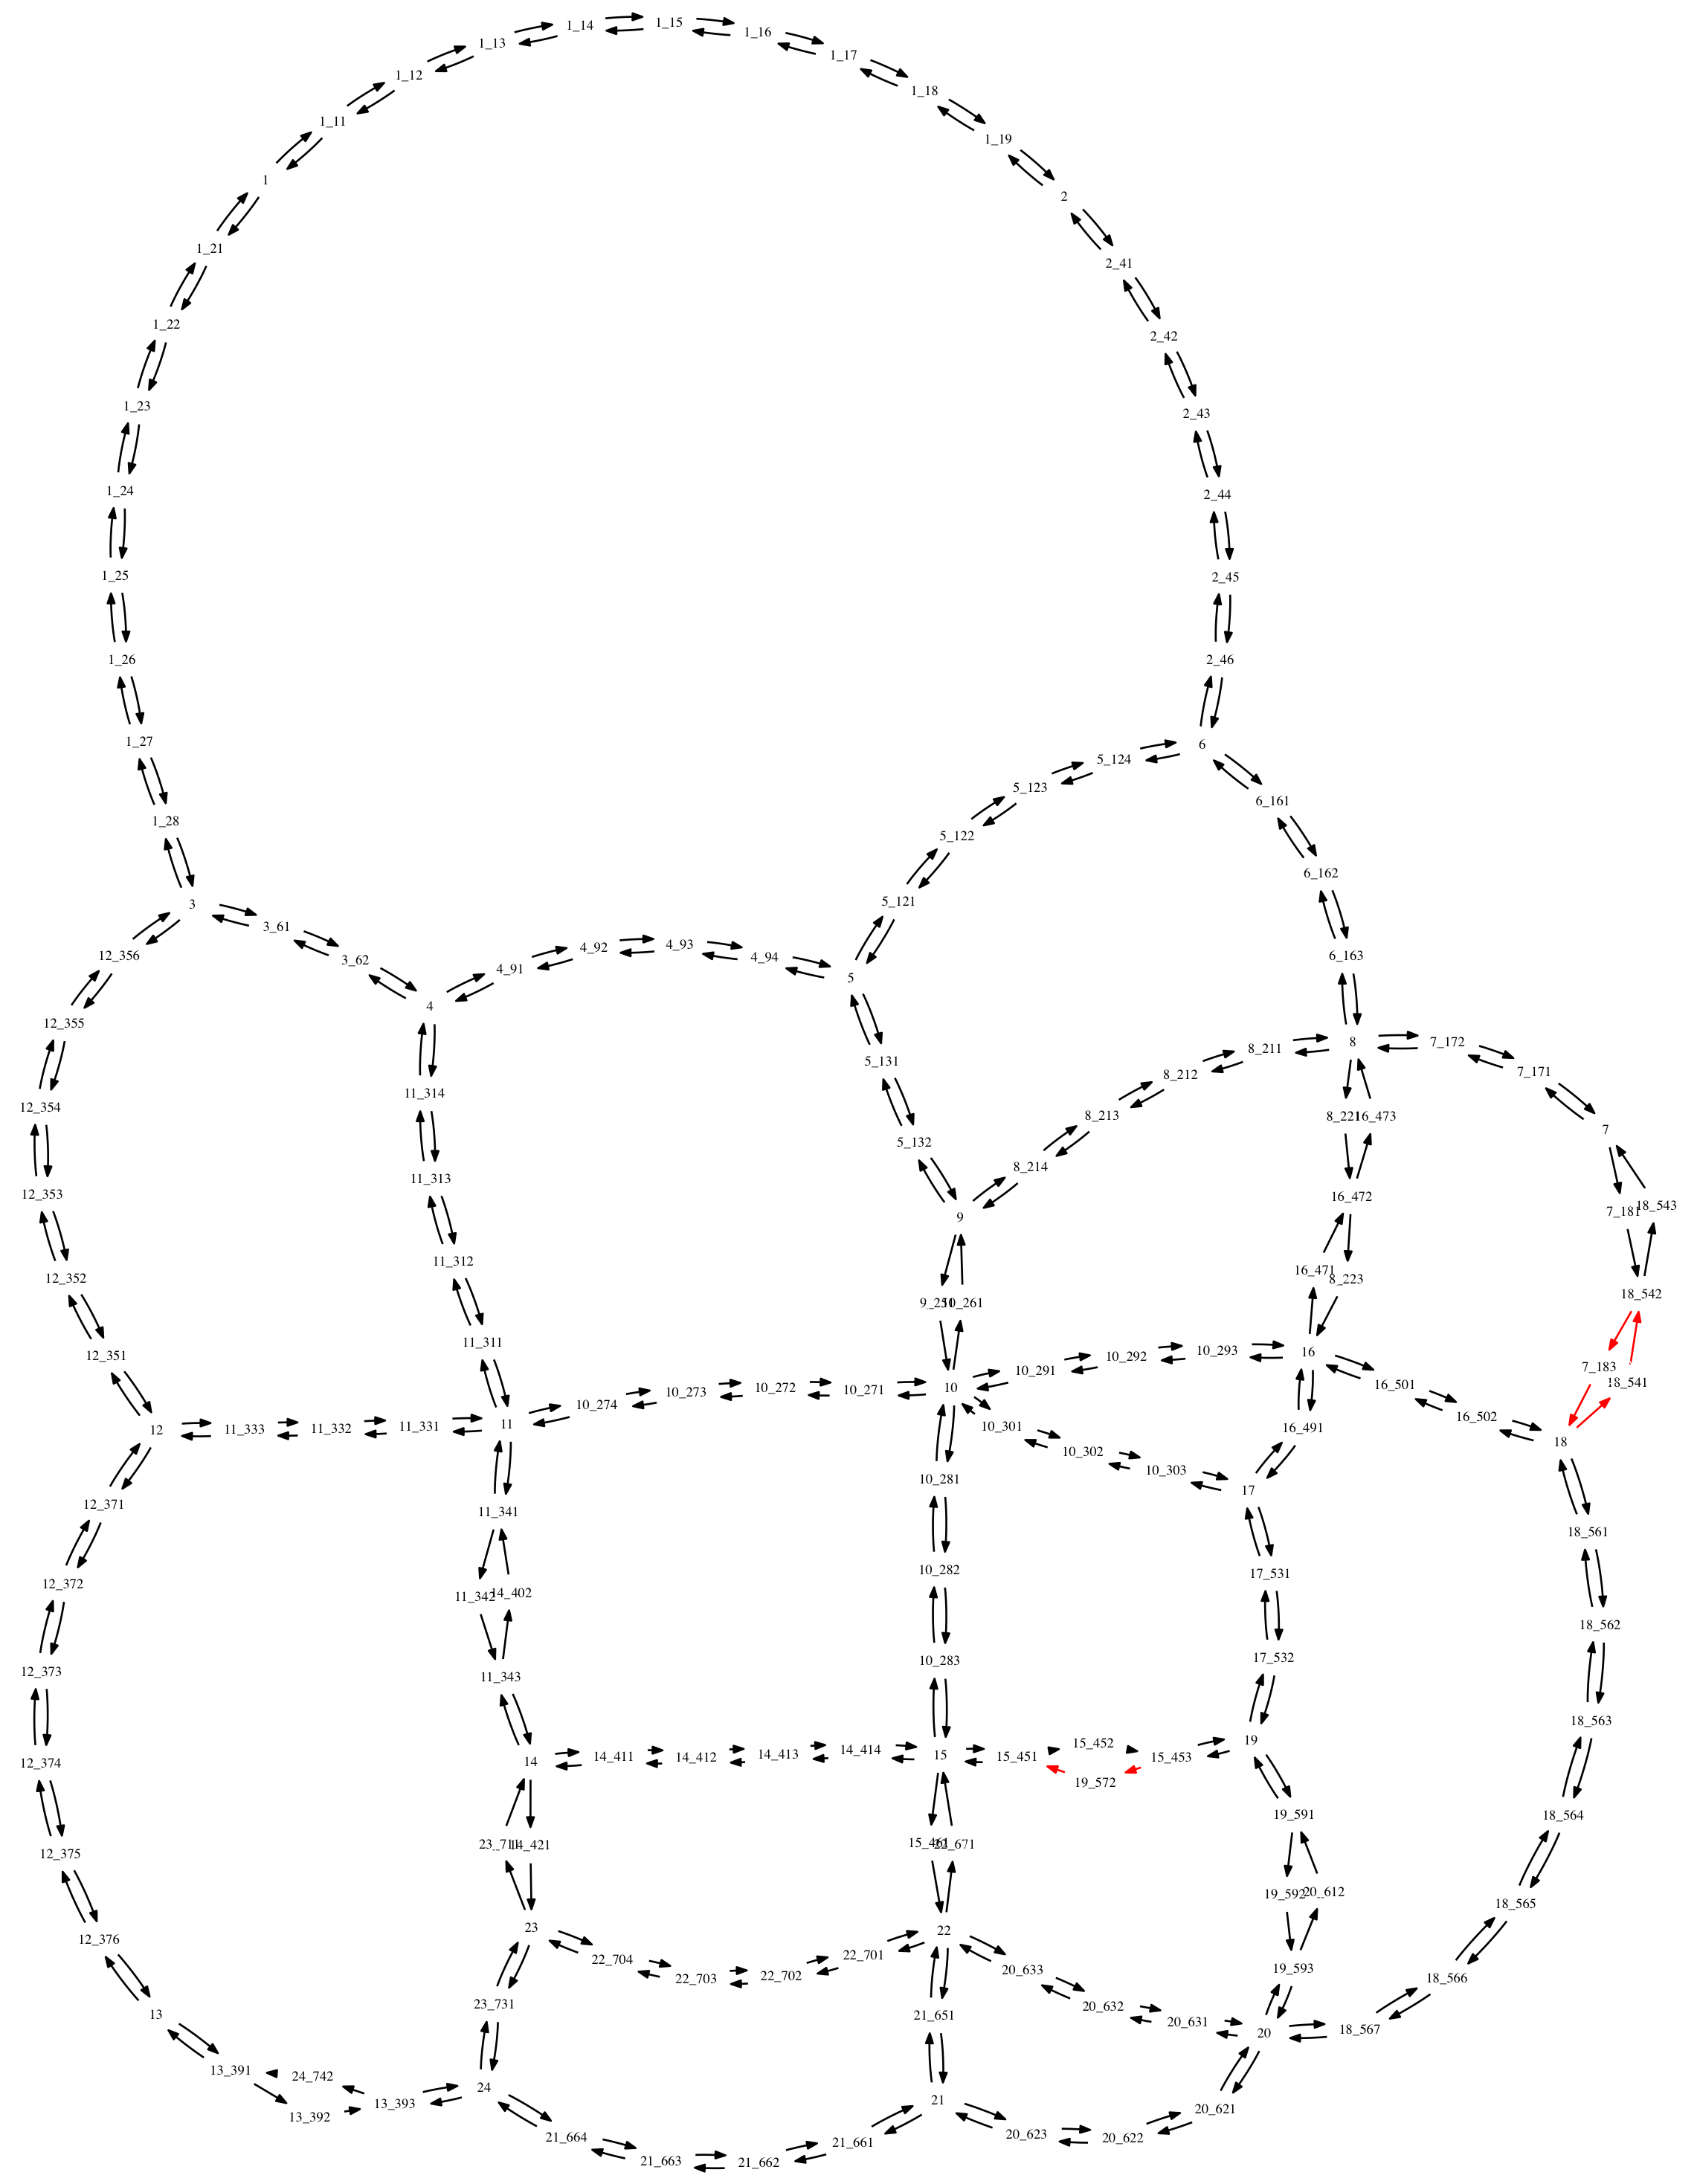
\includegraphics[totalheight=0.580\textheight, angle=90]{img/sioux-out/13/network2}
\caption{Sieć miasta Sioux Falls, rozwiązanie nr. 13.}
\label{sioux13}
\end{figure}

\begin{figure}[ht]
\centering
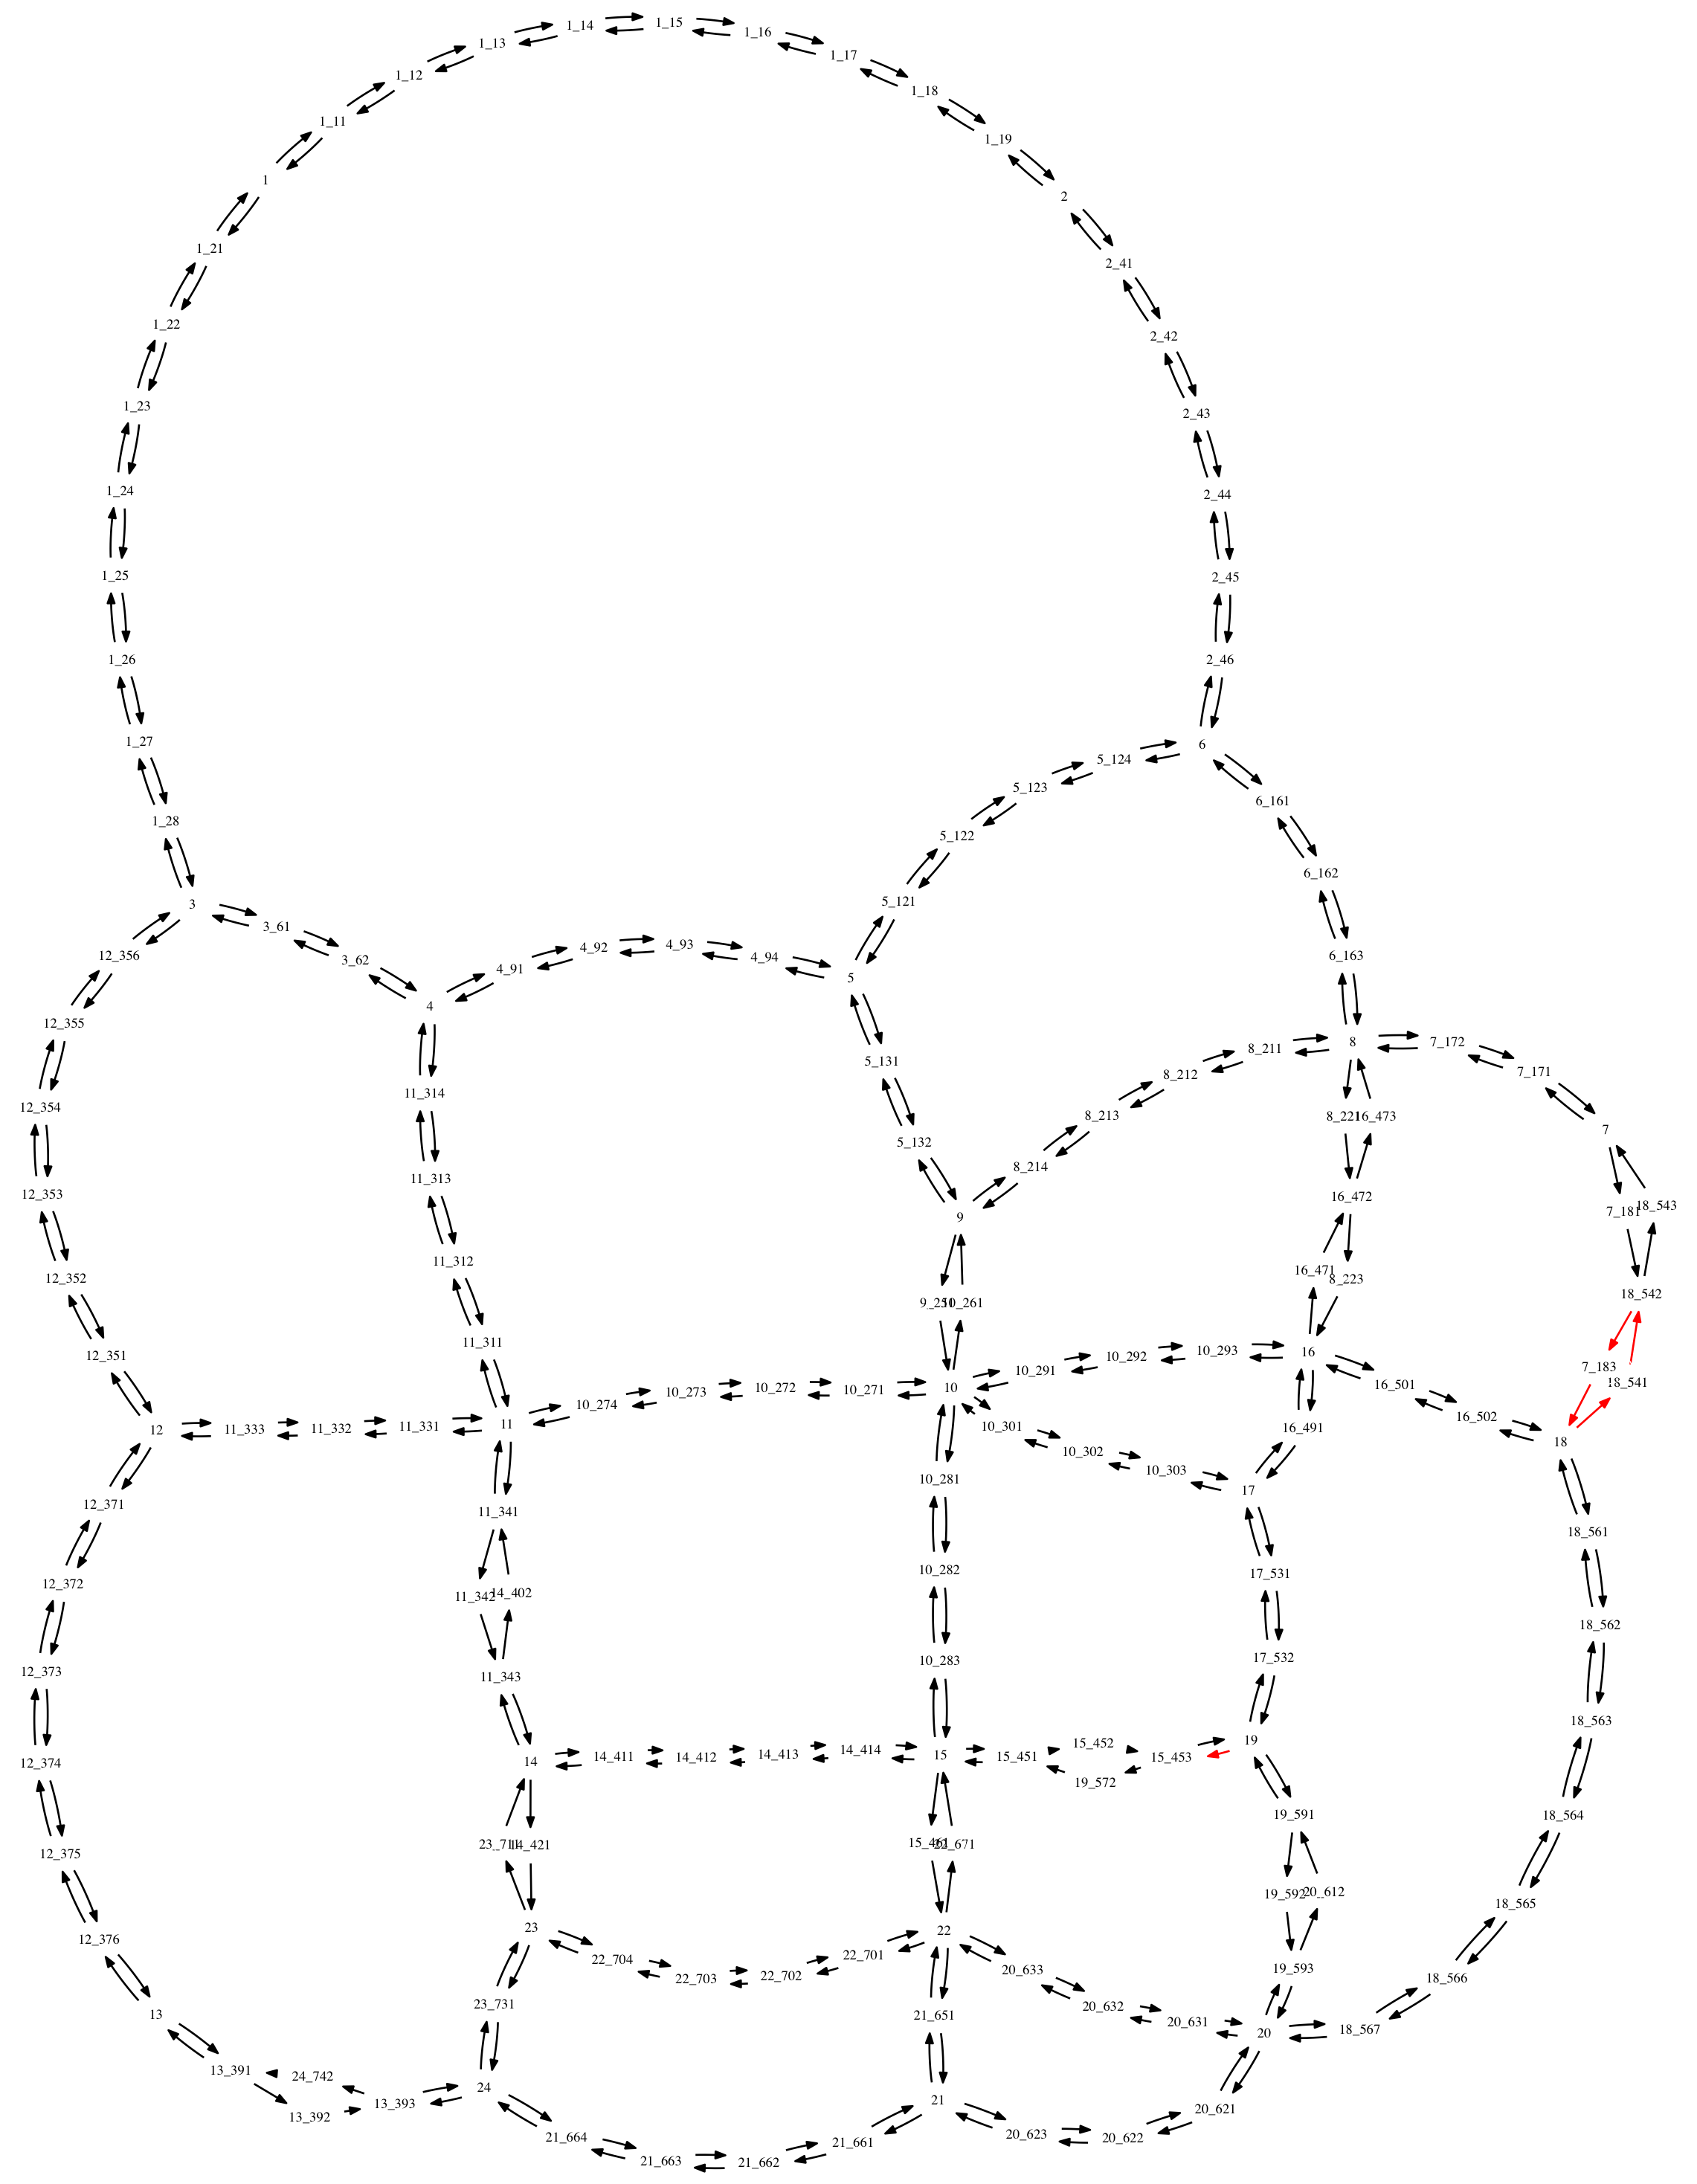
\includegraphics[totalheight=0.580\textheight, angle=90]{img/sioux-out/14/network2}
\caption{Sieć miasta Sioux Falls, rozwiązanie nr. 14.}
\label{sioux14}
\end{figure}

\begin{figure}[ht]
\centering
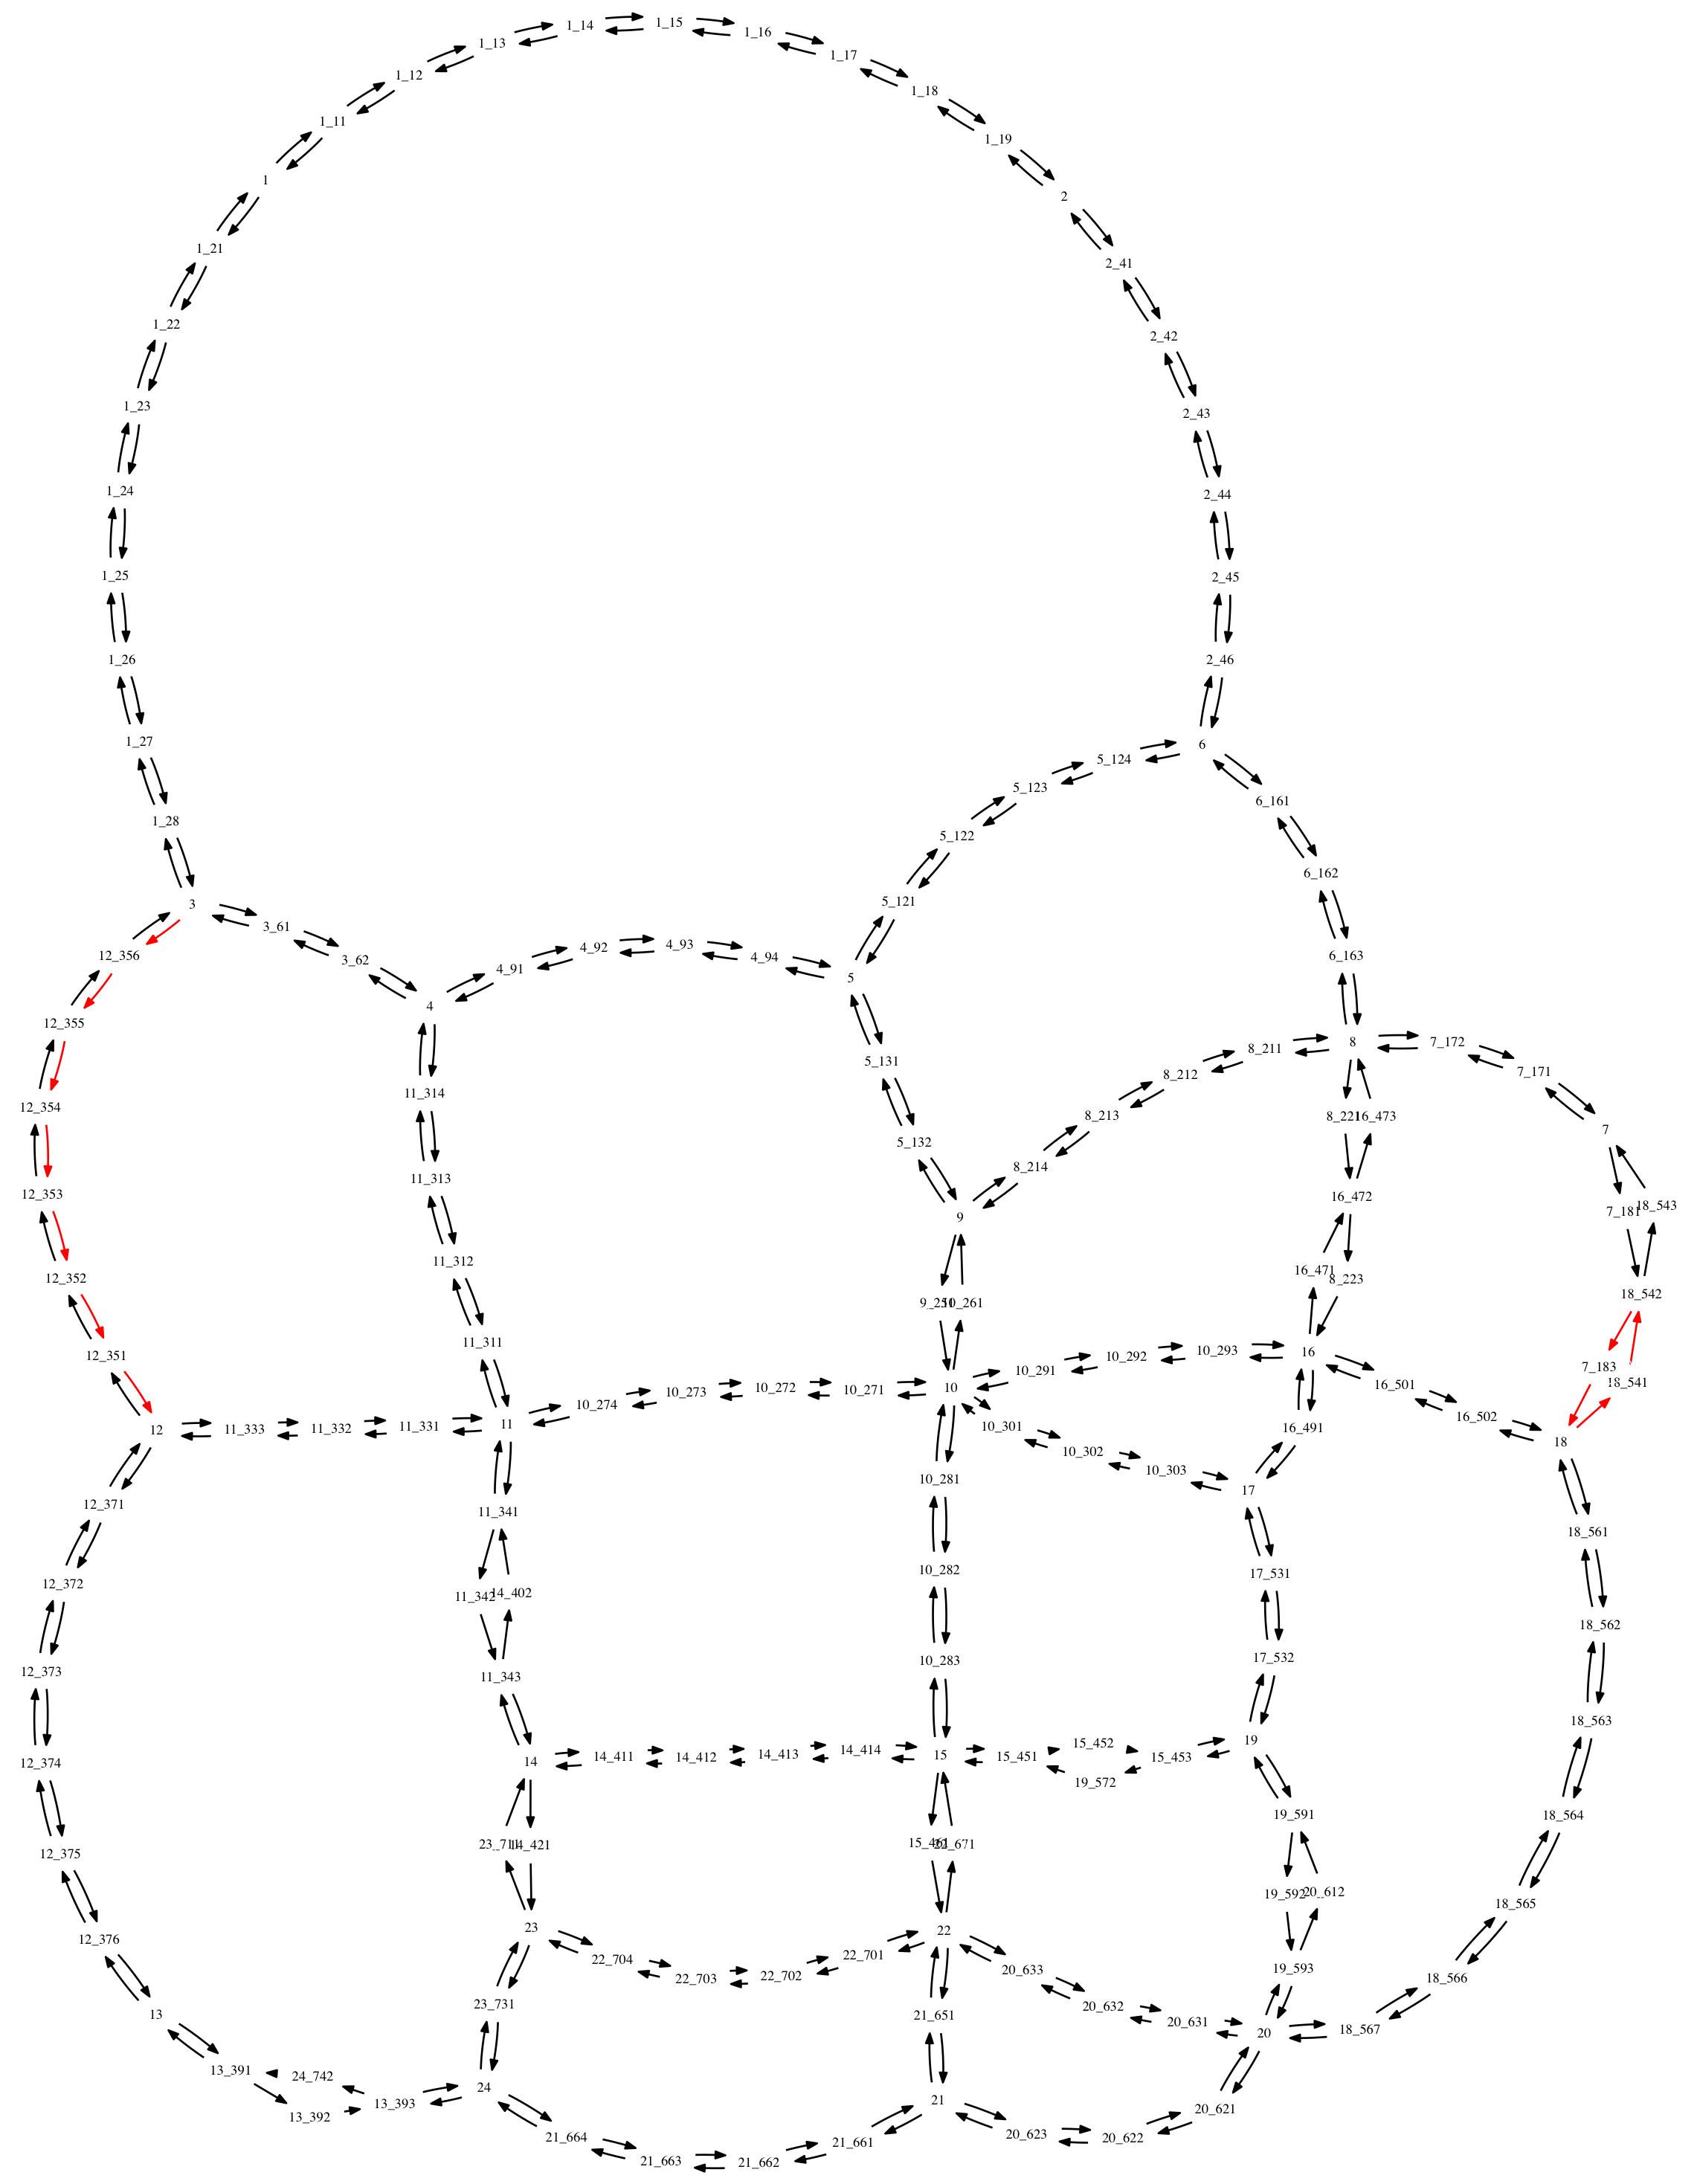
\includegraphics[totalheight=0.580\textheight, angle=90]{img/sioux-out/15/network2}
\caption{Sieć miasta Sioux Falls, rozwiązanie nr. 15.}
\label{sioux15}
\end{figure}

\begin{figure}[ht]
\centering
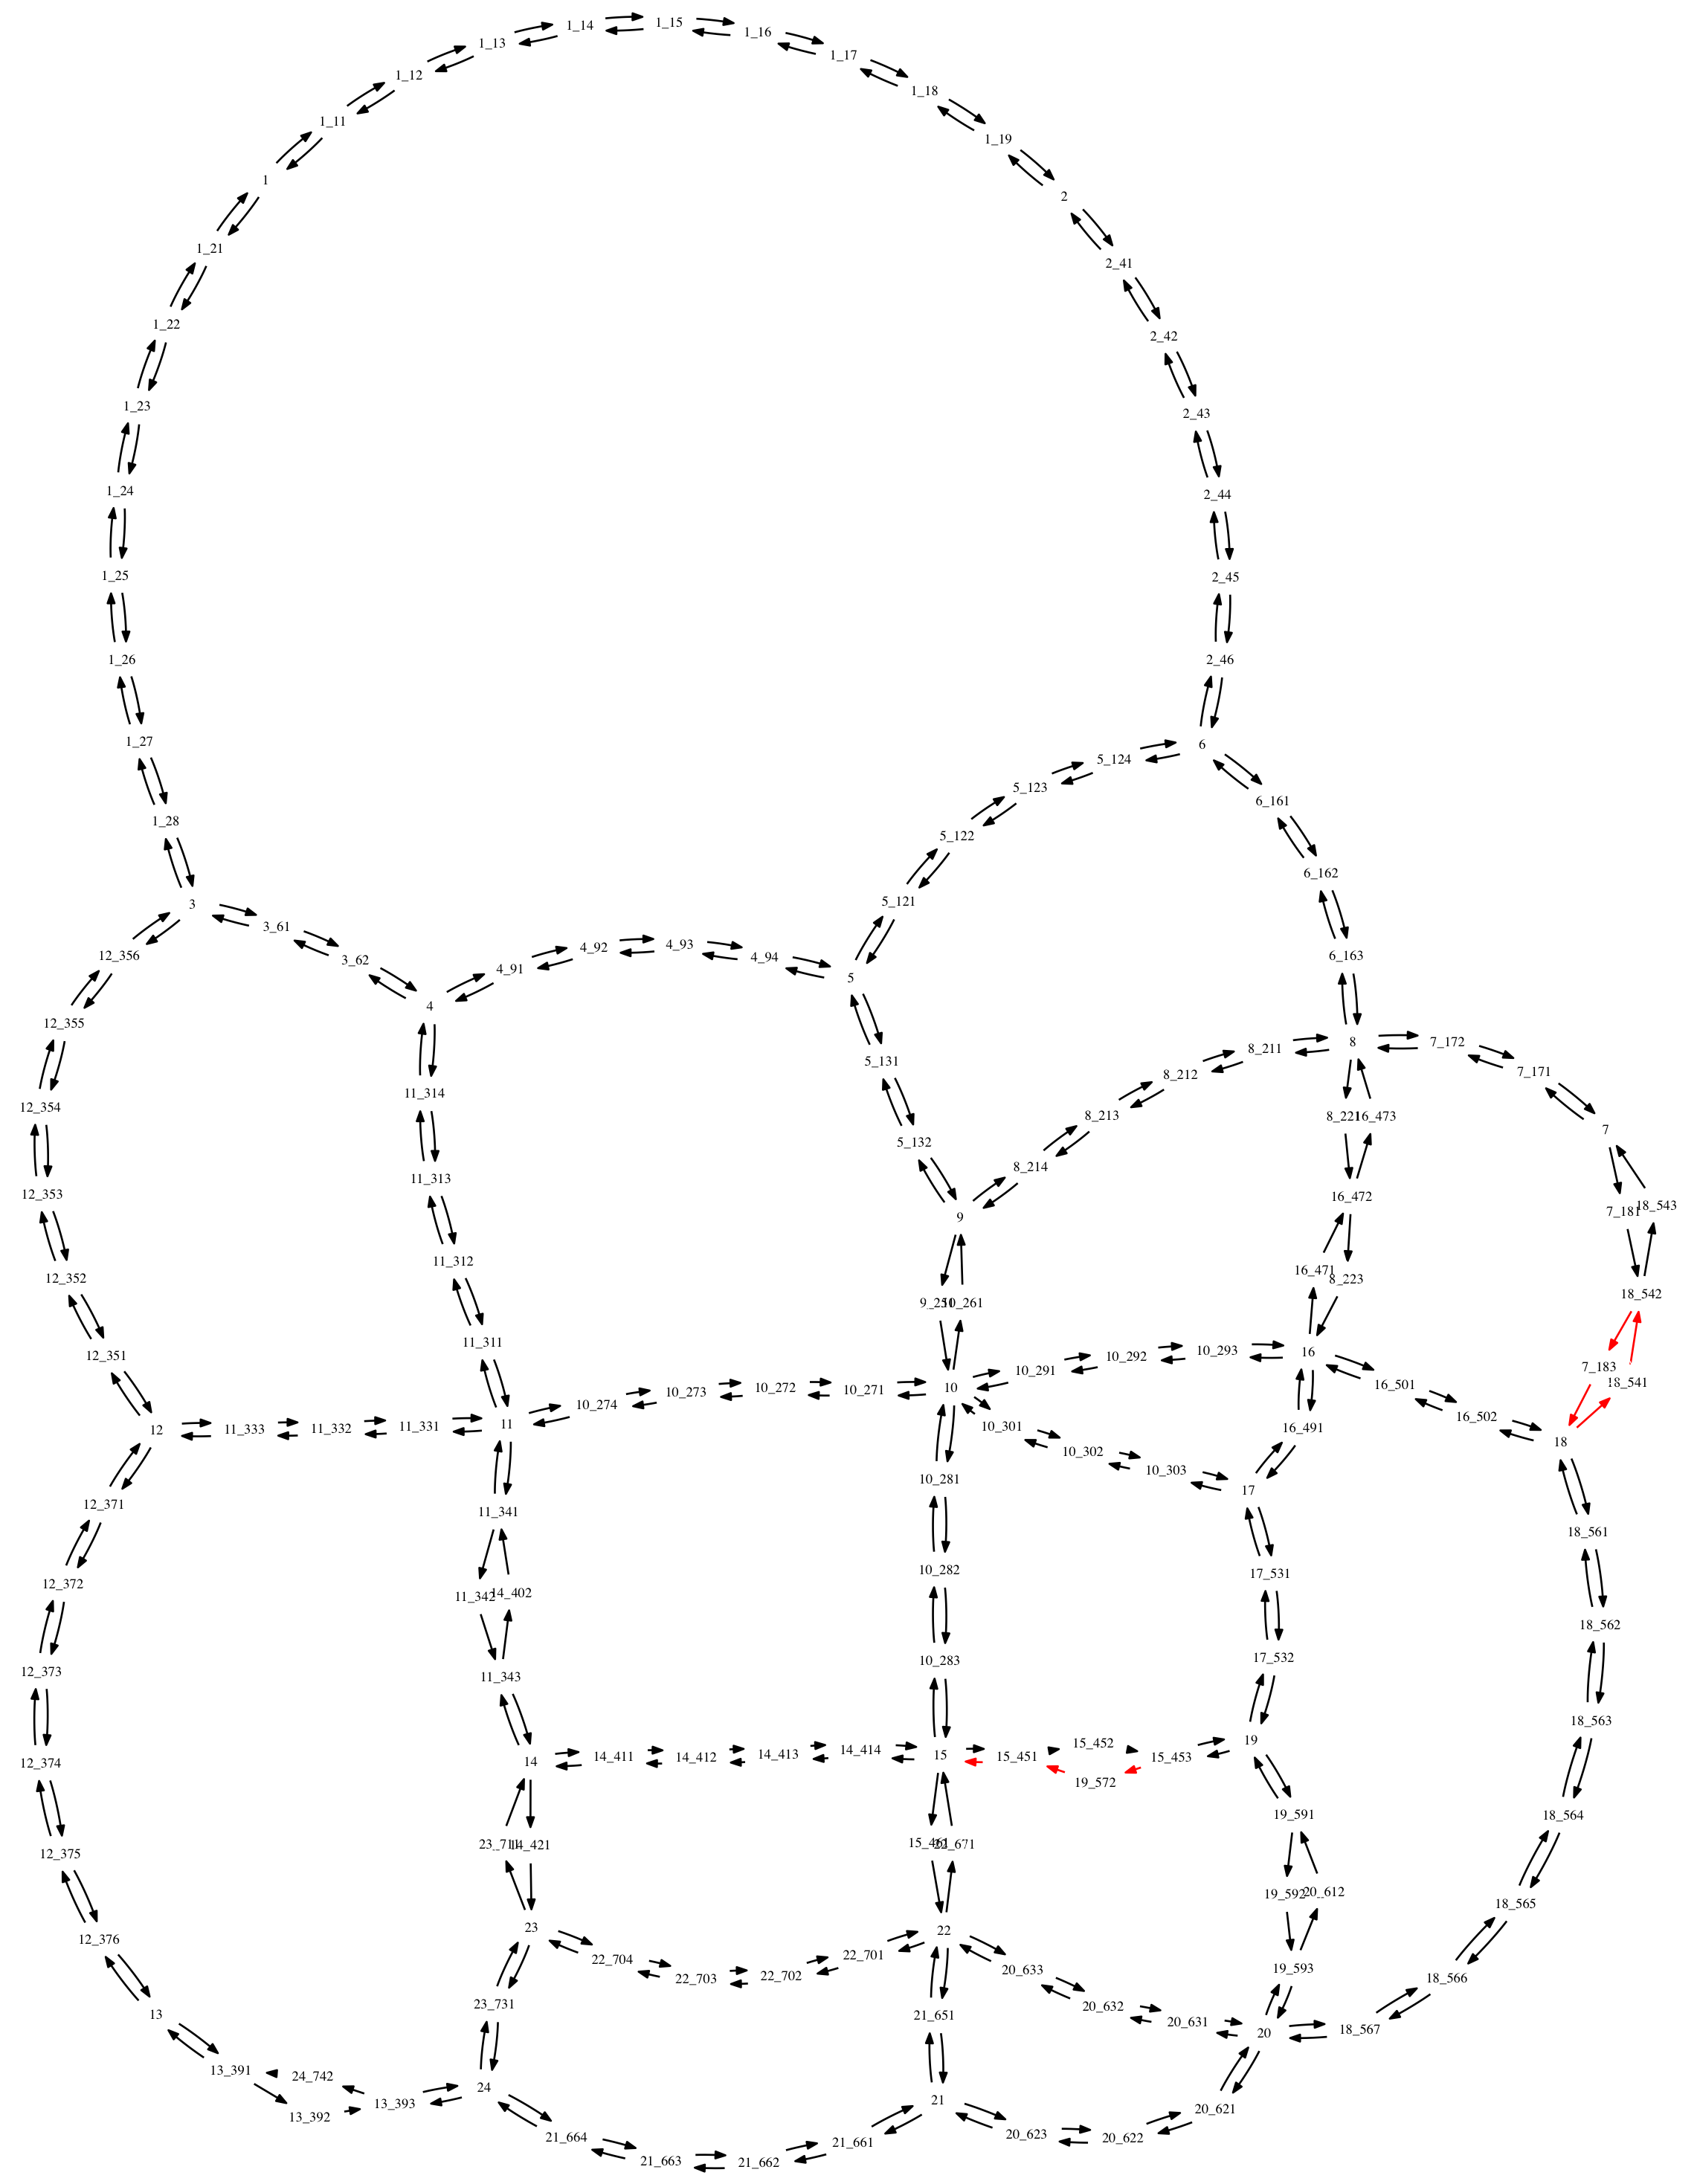
\includegraphics[totalheight=0.580\textheight, angle=90]{img/sioux-out/16/network2}
\caption{Sieć miasta Sioux Falls, rozwiązanie nr. 16.}
\label{sioux16}
\end{figure}

\begin{figure}[ht]
\centering
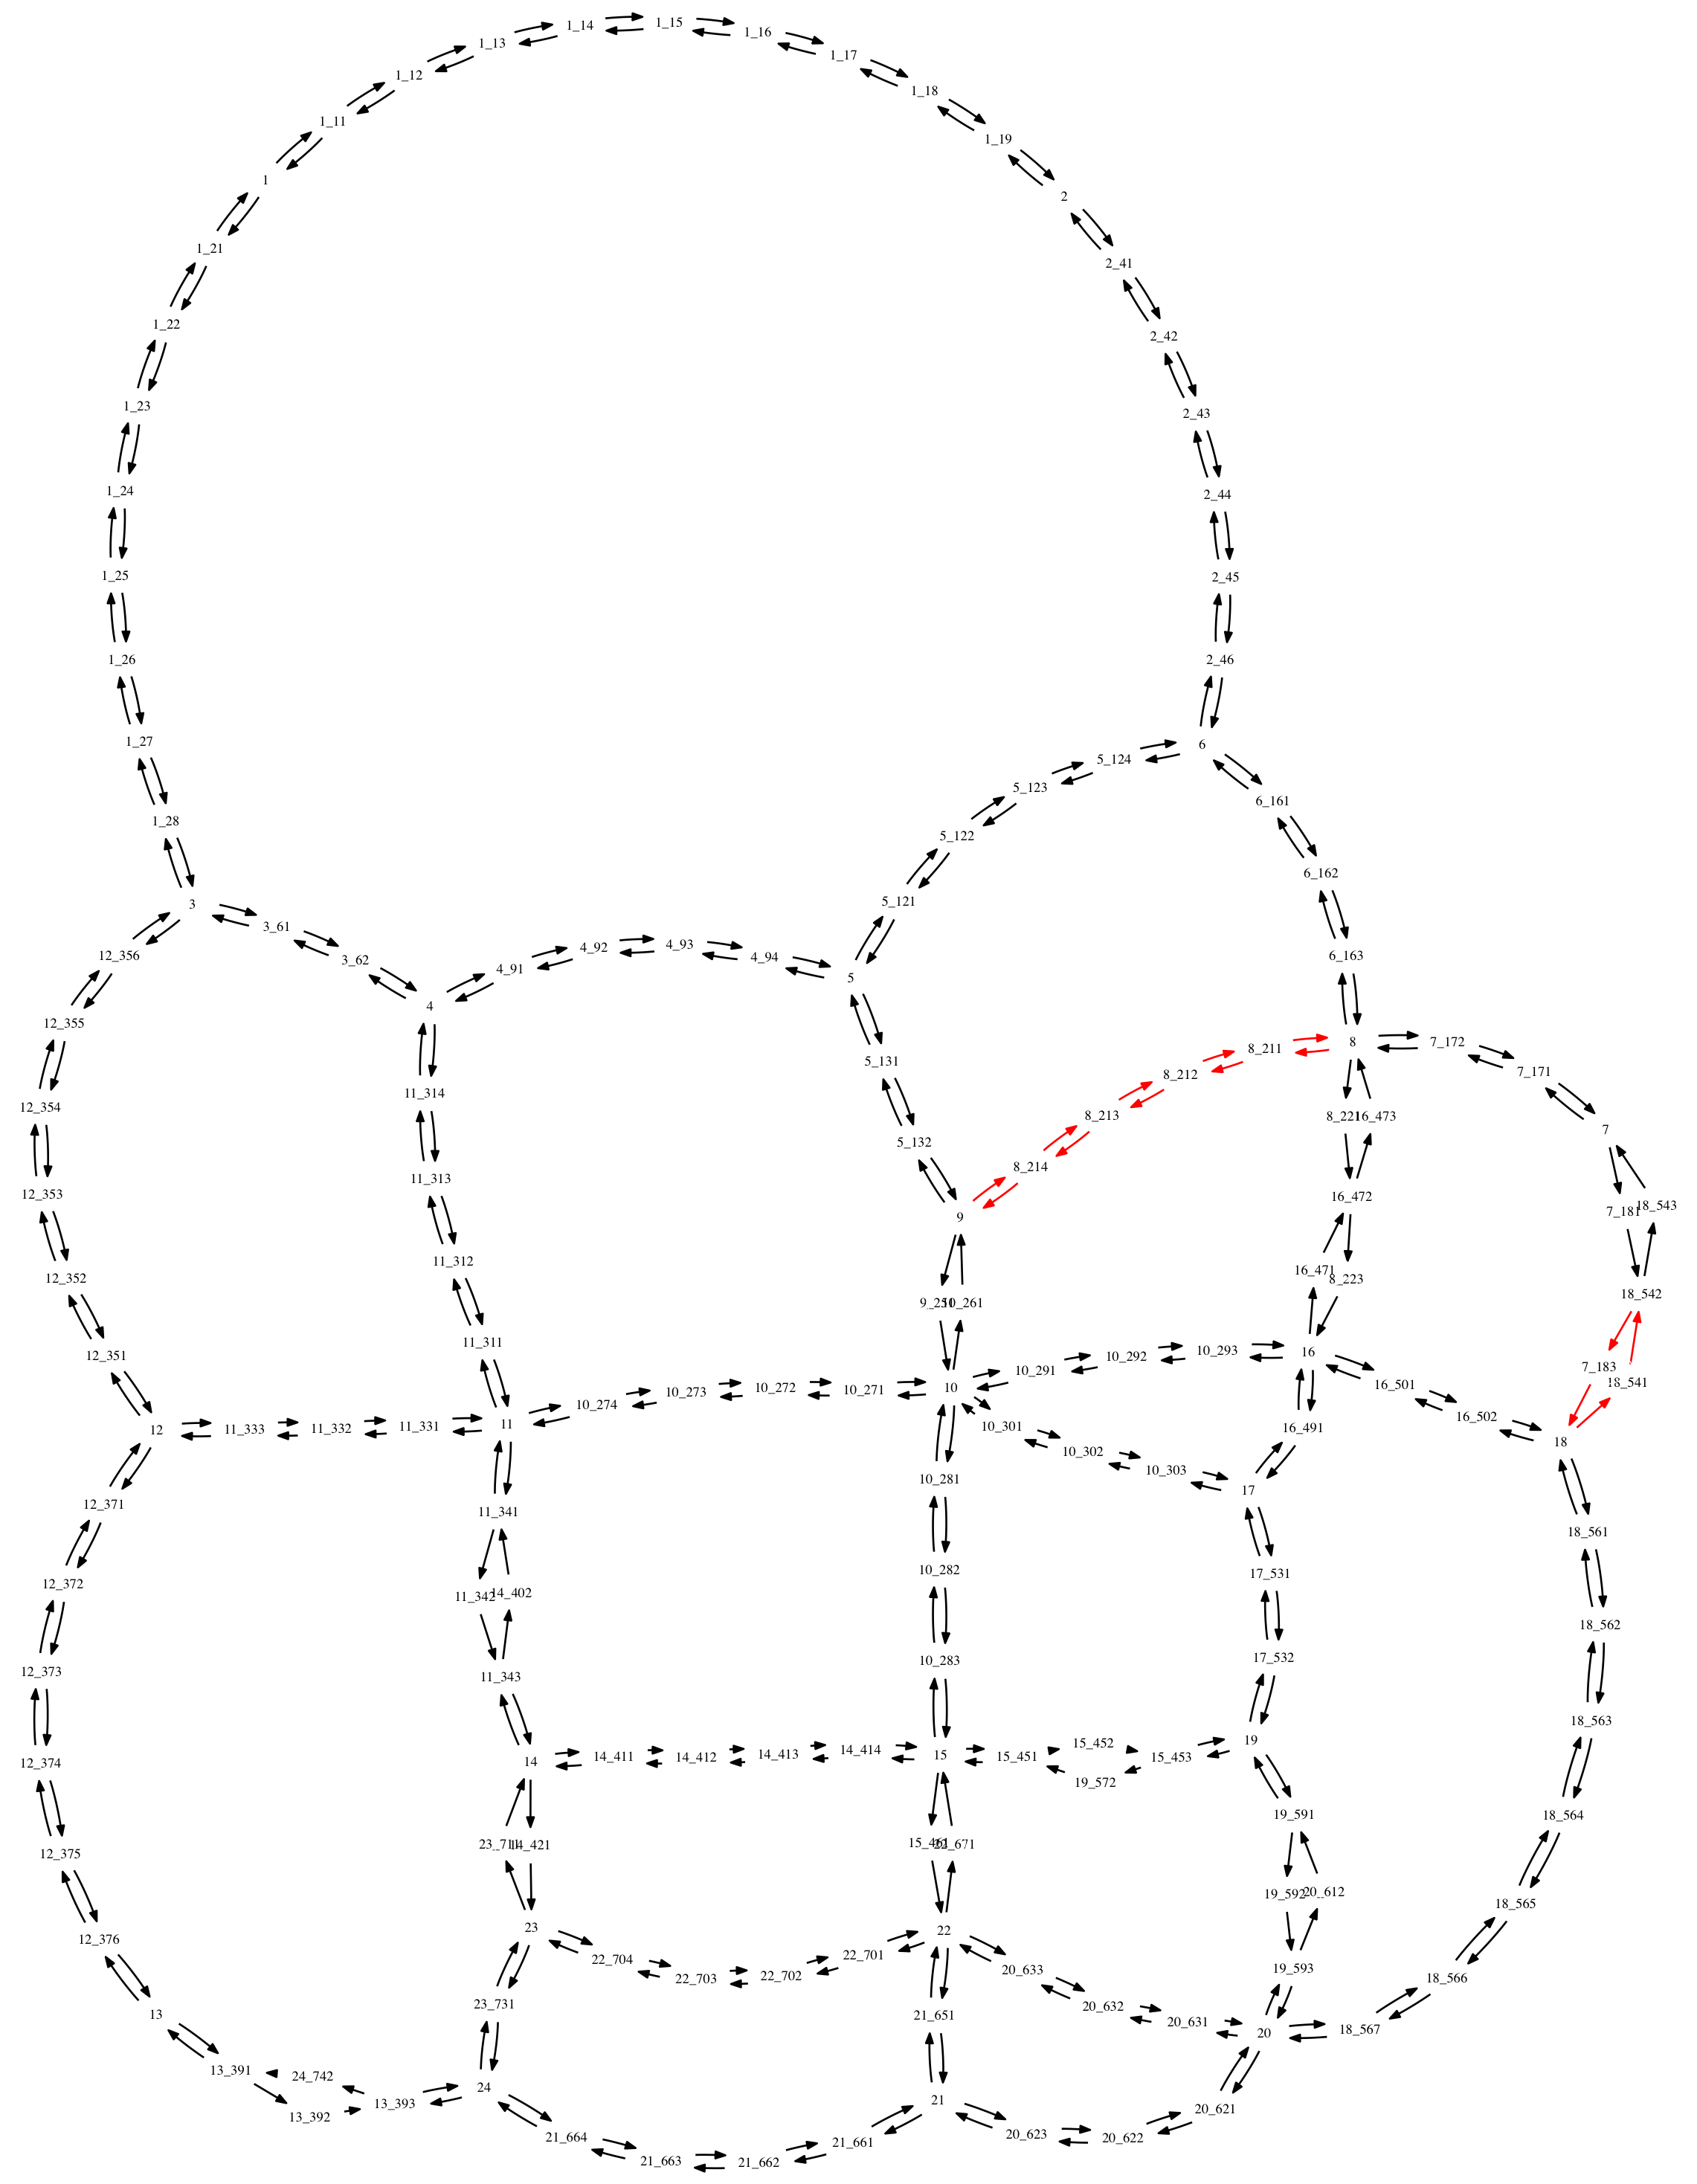
\includegraphics[totalheight=0.580\textheight, angle=90]{img/sioux-out/17/network2}
\caption{Sieć miasta Sioux Falls, rozwiązanie nr. 17.}
\label{sioux17}
\end{figure}

\clearpage
\section{Analiza symulacji}

Zgodnie z wcześniejszymi założeniami, podczas poszukiwań wybraliśmy ustawienie $10$ iteracji symulacji, do oceny sieci. W celu zweryfikowania wyników, dla najlepszych $17$ sieci przeprowadziliśmy ponowną symulację dla $100$ iteracji. Wyniki te porównujemy z wynikami sieci wejściowej. Rysunki \ref{iters1} - \ref{iters5} przedstawiają wyniki tych porównań. Dla poprawienia czytelności wykresy zostały rozdzielone. Numer sieci $0$ odnosi się do sieci wejściowej, natomiast pozostałe numery, do poszczególnych numerów ID sieci wybranych przez algorytm.

\begin{figure}[ht]
\centering
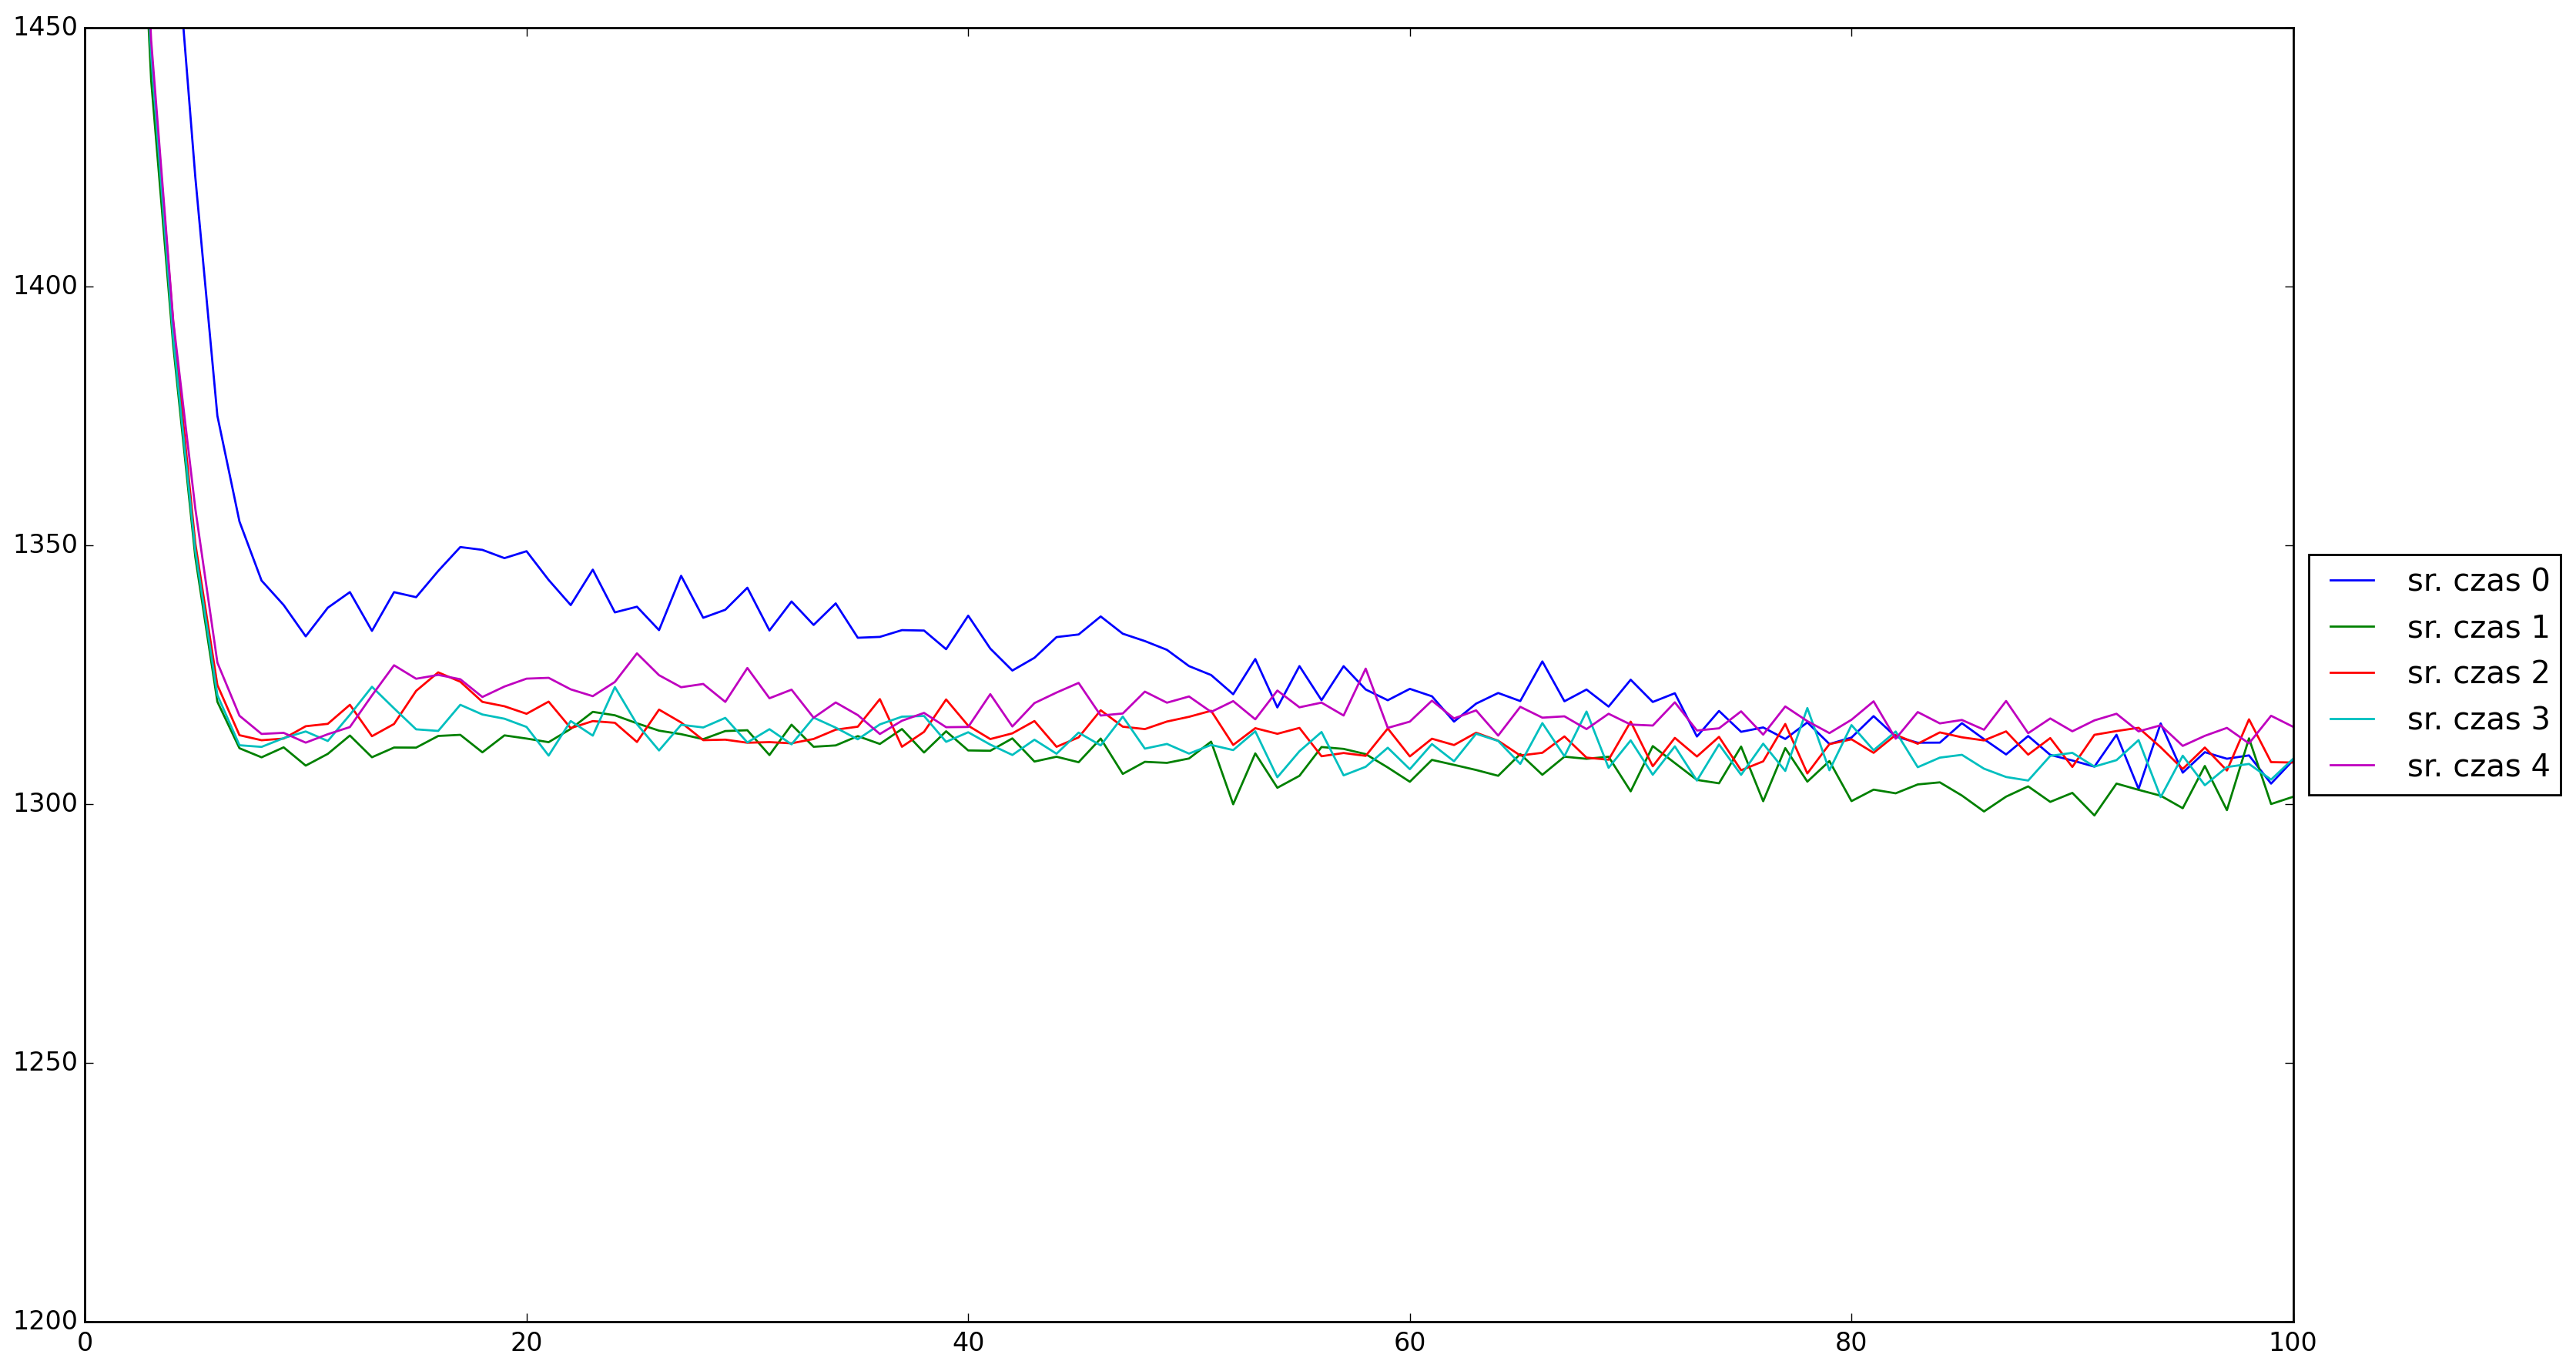
\includegraphics[width=1\textwidth]{img/iters/iters1}
\caption{Wykres zmiany średniego czasu przejazdu od iteracji dla sieci wynikowych z ujęciem sieci wejściowej.}
\label{iters1}
\end{figure}

\begin{figure}[ht]
\centering
\includegraphics[width=1\textwidth]{img/iters/iters2}
\caption{Wykres zmiany średniego czasu przejazdu od iteracji dla sieci wynikowych z ujęciem sieci wejściowej.}
\label{iters2}
\end{figure}

\begin{figure}[ht]
\centering
\includegraphics[width=1\textwidth]{img/iters/iters3}
\caption{Wykres zmiany średniego czasu przejazdu od iteracji dla sieci wynikowych z ujęciem sieci wejściowej.}
\label{iters3}
\end{figure}

\begin{figure}[ht]
\centering
\includegraphics[width=1\textwidth]{img/iters/iters4}
\caption{Wykres zmiany średniego czasu przejazdu od iteracji dla sieci wynikowych z ujęciem sieci wejściowej.}
\label{iters4}
\end{figure}

\begin{figure}[ht]
\centering
\includegraphics[width=1\textwidth]{img/iters/iters5}
\caption{Wykres zmiany średniego czasu przejazdu od iteracji dla sieci najlepszej z ujęciem sieci wejściowej.}
\label{iters5}
\end{figure}

\chapter{Podsumowanie.}\label{rozdz.podsumowanie} 
Uzyskane wyniki potwierdzają przede wszystkim badawczą stronę pracy. Dla zadanej sieci udało się zoptymalizować ruch drogowy, stosując zamknięcie określonych węzłów. Trzeba jednak pamiętać, co już zostało wspomniane, że wynik jest czysto teoretyczny. Symulacja nie odzwierciedla prawdziwego ruchu drogowego w~mieście a~ponadto zastosowaliśmy jedynie uproszczenie, w~którym nie są obecne wszystkie węzły rzeczywistej sieci drogowej. W~związku z~powyższym, uzyskane wyniki, można traktować co najwyżej jako sugestię. 

\section{Dyskusja wyników.}
Gdyby założyć, że system ten miałby dostarczyć pewnej sugestii w~sprawie podjęcia decyzji dotyczącej usprawnienia ruchu, spełnia on swoje zadanie. Przeszukiwanie przestrzeni rozwiązań wykorzystując algorytmy genetyczne, nie jest może najefektywniejszym przykładem, jednak skutecznym. Działanie podparte sumienną symulacją może przekazać miarodajne wyniki.

Symulator MATSim zadziałał zgodnie z oczekiwaniami, wykazując dużą zdolność adaptacji agentów do sieci. Przypadek ten można opisać, zadając sobie pytanie, skąd właściwie biorą się korki i zatory drogowe? Są one zwykle efektem braku poprawnego planu podróży uczestników ruchu. Symulator potrafi znaleźć taki plan, który w sposób idealny, dobiera czas podróży oraz najlepszą drogę. Jest to oczywiście możliwe dzięki powtarzającym się w każdej iteracji \textbf{tym samym} warunkom drogowym panującym w sieci. Nie jest to więc sytuacja rzeczywista.

Mając na uwadze powyższe, wybory w iteracjach wcześniejszych są mniej idealne, można powiedzieć, bardziej ludzkie. Wykresy \ref{iters1} - \ref{iters5} wyraźnie pokazują, że dla zmodyfikowanej sieci, znacznie trudniej jest popełnić błąd przy planowaniu trasy, mając ograniczoną wiedzę na temat warunków drogowych. Wymuszenie więc określonych dróg na agentach pozwoliło im szybciej dokonywać prawidłowych wyborów.

W przypadku długiej symulacji, część sieci zmodyfikowanych osiągała gorszy rezultat niż sieć wejściowa. Oprócz wyżej wymienionych czynników, musimy bowiem pamiętać, że generalnie większa liczba węzłów oznacza większe możliwości przepływowe sieci. Efekt dłuższej symulacji można porównać z dopasowaniem sieci drogowej do potrzeb zadanego modelu agentów. Taka sieć spełniałaby idealnie wymogi danej symulacji. Nie sprawdziłaby się, jednak gdyby model został zmieniony. W przypadku długiej nauki agentów, na temat danej sieci, mamy sytuację odwrotną.

\section{Analiza wyników.}
Pierwszym krokiem, który pomaga w~analizie otrzymanych wyników jest ich zgrupowanie. Dość intuicyjnym jest grupowanie na zbiory, zamykające podobne obszary (węzły). Na pierwszy rzut oka widać wyraźną zbieżność w~jednym rejonie. Niestety, choć zdecydowanie musi mieć on wpływ na poprawę czasu symulacji, nie wydaje się on punktem ,,strategicznym'' komunikacji miejskiej. Mowa oczywiście o~zamknięciu węzłów między $18$ i~$18\_542$. Przedstawiamy zaznaczony fragment na rysunku \ref{frag_1}, obróconym o~$90^{\circ}$ w~lewo.

\begin{figure}[ht]
\centering
\includegraphics[width=0.4\textwidth, angle=90]{img/sioux-out/obszar1}
\caption{Fragment grafu z zaznaczonym obszarem 1.}
\label{frag_1}
\end{figure}

Ciekawym jest jednak obszar wspólny dla wyników \ref{sioux5}, \ref{sioux7}, \ref{sioux9}, \ref{sioux10}, \ref{sioux11}, \ref{sioux12}, \ref{sioux13}, \ref{sioux14}, \ref{sioux16}. Jest to obszar znajdujący się pomiędzy wspomnianymi wierzchołkami $15$ i~$19$. Przedstawiamy zaznaczony fragment na rysunku \ref{frag_2}.

\begin{figure}[ht]
\centering
\includegraphics[width=0.60\textwidth]{img/sioux-out/obszar2}
\caption{Fragment grafu z zaznaczonym obszarem 2.}
\label{frag_2}
\end{figure}

Drugim obszarem, który został wybrany w~przypadku paru rozwiązań, są ulice pomiędzy skrzyżowaniem (wierzchołkiem) $5$ i~$6$. Został on wybrany przez \ref{sioux2}, \ref{sioux4}, \ref{sioux6}, \ref{sioux8}, \ref{sioux12}. Przedstawiamy zaznaczony fragment na rysunku \ref{frag_3}.

\begin{figure}[ht]
\centering
\includegraphics[width=0.65\textwidth]{img/sioux-out/obszar3}
\caption{Fragment grafu z zaznaczonym obszarem 3.}
\label{frag_3}
\end{figure}

Ostatni obszar, który charakteryzował się wspólnym wynikiem dla więcej niż jednego rozwiązania, tj: \ref{sioux3}, \ref{sioux8}, \ref{sioux15} znajduje się pomiędzy wierzchołkiem $3$ i~$12$. Przedstawiamy zaznaczony fragment na rysunku \ref{frag_4}, obróconym o~$90^{\circ}$ w~lewo.

\begin{figure}[ht]
\centering
\includegraphics[width=0.35\textwidth, angle=90]{img/sioux-out/obszar4}
\caption{Fragment grafu z zaznaczonym obszarem 4.}
\label{frag_4}
\end{figure}

Powyższe sugestie mogą zostać użyte w~celu poszerzonych badań nad danymi obszarami, decydując czy faktycznie mają one wpływ na komunikację w~mieście. Otrzymane wyniki nie oznaczają również, że nie istnieje bardziej optymalne rozwiązanie. Przestrzeń przeszukiwań dla powyższego grafu wynosiła $2^{90}$, a~więc zbadanie wszystkich możliwych rozwiązań problemu jest praktycznie niewykonalne.

\clearpage
\section{Perspektywy dalszych badań w~dziedzinie.}
Dość oczywistym kierunkiem rozwoju może być oczywiście dalsze przeszukiwanie posiadanego problemu. Jak już zostało wspomniane wyżej, ilość dostępnych rozwiązań jest bardzo duża.

Ciekawszym wydaje się być jednak przeszukiwanie nowych zbiorów. W~przypadku symulatora MATSim mamy do swojej dyspozycji dość pokaźną liczbę przykładów opartych o~rzeczywiste miasta, na których były prowadzone symulacje. Jeden z~dostępnych modeli jest odwzorowaniem miasta Berlin, przy okazji, wykonanym z~dużo większą dokładnością niż Sioux Falls \ref{berlin}.

\begin{figure}[ht]
\centering
\includegraphics[width=\textwidth]{img/berlin2}
\caption{Sieć drogowa miasta Berlin w postaci grafu.}
\label{berlin}
\end{figure}

Ponadto, w~pracy można wykorzystać inne twierdzenia i~paradoksy dotyczące m.in. transportu miejskiego. Niestety, jak już było wspomniane wcześniej, wiele z~tych praw jest opartych o~psychologiczne tezy, bez matematycznego podparcia, co powoduje, że wyniki są trudne do przewidzenia.

\section{Struktura projektu.}

Załączone na płycie źródła pozwalają na odtworzenie pełnego projektu używając wymienionych wcześniej środowisk programistycznych, Eclipse \cite{eclipse} i~PyDev \cite{pydev}. Poniżej przedstawiona zostaje struktura katalogów, w~kolejności alfabetycznej, wraz z~krótkim opisem zawartości.

\subsubsection{fakematsim/}
Jest to sztuczna implementacja symulatora pozwalająca na testowanie działania algorytmu genetycznego w~oparciu o~losowe wyniki. Działanie opiera się o~rozpakowanie gotowego folderu z~wcześniej przygotowanymi obliczeniami oraz podmianę wyniku na losową liczbę. Projekt jest przygotowany w~oparciu o~strukturę projektu \textit{Maven}. Jego skompilowane źródła znajdują się  w~katalogu \textit{matsim}.

\subsubsection{java/}
Tutaj znajduje się główny projekt zarządzający aplikacją obliczeniową. Jest on przygotowany w~oparciu o~strukturę projektu \textit{Maven}. Zawiera przykładowe pliki konfiguracyjne i~przygotowane testy \textit{JUnit} pozwalające na ich bezpośrednie wykorzystanie.

\subsubsection{literature/}
W tym folderze zostały zebrane wszystkie źródła literaturowe wykorzystane przy tworzeniu pracy.

\subsubsection{matsim/}
Folder ten zawiera skompilowane wersje symulatora MATSim oraz jego falsyfikatu wykorzystywanego podczas testów. Symulator został skompilowany ze źródeł dostępnych na repozytorium głównym projektu\footnote {\url{https://svn.code.sf.net/p/matsim/source/matsim/trunk}}. Drobne modyfikacje dotyczyły tylko parametrów logowania oraz uruchomienia symulatora. Nie zostały dokonane żadne zmiany ingerujące w~przebieg samej symulacji.

\subsubsection{sioux-out/}
Jest to domyślny katalog z~danymi otrzymanymi w~wyniku działania projketu.

\subsubsection{paper/}
Katalog ze źródłami pracy pisemnej w~formacie TeX.

\subsubsection{python/}
Znajdują się tutaj wszystkie wykorzystane w~projekcie skrypty Python wraz z~testami jednostkowymi. Jest to również katalog domyślny wywołań skryptów podczas obliczeń.

\subsubsection{README.md}
Plik zawierający opis instalacji wymaganych przez projekt zależności i~bibliotek na podstawie systemu Linux Ubuntu 12.04 LTS.

\subsubsection{scenarios/}
Zawiera przykładowe scenariusze, które mogą być wykorzystane przy pracy z~symulatorem MATSim. Znajduje się tutaj, oprócz wykorzystanego miasta Sioux Falls, Berlin i~Bruksela. Ponadto zawiera parę przykładowych plików konfiguracyjnych symulatora.

\subsubsection{seminar/}
Zawiera prezentację wykorzystaną podczas seminarium dyplomowego, przedstawiającą wstępne założenia projektu.


\cleardoublepage
\phantomsection
\addcontentsline{toc}{chapter}{\listfigurename} 
\listoffigures

\cleardoublepage
\phantomsection
\addcontentsline{toc}{chapter}{\listtablename} 
\listoftables

\cleardoublepage
\phantomsection
\addcontentsline{toc}{chapter}{\lstlistlistingname}
\lstlistoflistings

\cleardoublepage
\phantomsection
\addcontentsline{toc}{chapter}{\bibname} 
\begin{thebibliography}{99}
\bibitem{investigation} 
	Leslie Arthur Keith Bloy, 
	\newblock \textit{An investigation into Braess’ paradox}, 02/2007

\bibitem{newinsights}
	Rric Pas and Shari Principio
	\newblock \textit{Braess’ paradox: Some new insights}, April 1996

\bibitem{conference} 
	Wataru Nanya, Hiroshi Kitada, Azusa Hara, Yukiko Wakita, Tatsuhiro Tamaki, and Eisuke Kita
	\newblock \textit{Road Network Optimization for Increasing Traffic Flow}
	\newblock Int. Conference on Simulation Technology, JSST 2013.

\bibitem{reducingtheeffects}
	Ana L.~C.~Bazzan and Franziska Klügl
	\newblock \textit{Reducing the Effects of the Braess Paradox with Information Manipulation}

\bibitem{paradox}
	Dietrich Braess. 
	\newblock \textit{Über ein Paradoxon aus der Verkehrsplanung. „Unternehmensforschung”.} 
	\newblock 12, s.~258–268, 1968 (niem.).

\bibitem{gene}
	Mitchell Melanie
	\newblock \textit{An Introduction to Genetic Algorithms}
	\newblock First MIT Press paperback edition, 1998

\bibitem{matsim userg}
	M.~Rieser, C.~Dobler, T.~Dubernet, D.~Grether, A.~Horni, G.~Lammel, R.~Waraich, M.~Zilske, Kay W.~Axhausen, Kai Nagel
	\newblock \textit{MATSim User Guide}
	\newblock updated September 12, 2014

\bibitem{siux}
	A.~Chakirov
	\newblock \textit{Enriched Sioux Falls Scenario with Dynamic Demand}
	\newblock MATSim User Meeting, Zurich/Singapore, June 2013.
	
\bibitem{grafy}
	Łukasz Kowalik
	\newblock \textit{Algorytmy i~struktury danych, grafy}
	\newblock Wykład, 2003.
	
\bibitem{genetyczne}
	Marta Grzanek
	\newblock \textit{Sztuczna inteligencja, Klasyczny algorytm genetyczny}
	\newblock Wykład, 2007.
	
\bibitem{gene mutikrzyz}
	Dilvan de Abreu Moreira
	\newblock \textit{Agents: A~Distributed Client/Server System for Leaf Cell Generation}
	\newblock Thesis, 1995
	
\bibitem{matsim} 
	\url{http://matsim.org}	

\bibitem{math}
	\url{http://commons.apache.org/proper/commons math}
	
\bibitem{networkx}
	\url{http://networkx.github.io}

\bibitem{java} 
	\url{http://www.java.com/pl/}

\bibitem{eclipse} 
	\url{https://eclipse.org}
				
\bibitem{python} 
	\url{http://pl.python.org}
	
\bibitem{pydev} 
	\url{http://pydev.org}
	
\bibitem{ubuntu}
	\url{http://www.ubuntu.com}
	
\bibitem{azure}
	\url{http://azure.microsoft.com}
			
\bibitem{braess}
	\url{http://pl.wikipedia.org/wiki/Paradoks_Braessa}
	
\bibitem{urban}
	\url{http://urbnews.pl/paradoks braessa/}
	
\bibitem{downs}
	\url{http://pl.wikipedia.org/wiki/Paradoks_Downsa Thomsona}
	
\bibitem{lewis}
	\href{http://pl.wikipedia.org/wiki/Prawo_Lewisa Mogridge\%E2\%80\%99a}
	    {http://pl.wikipedia.org/wiki/Prawo\_Lewisa Mogridge\textquoteright{}a}
	   
\bibitem{silniespojny}
	\url{http://mathworld.wolfram.com/StronglyConnectedDigraph.html}

\end{thebibliography}

\cleardoublepage
\phantomsection
\addcontentsline{toc}{chapter}{Abstract}
\chapter*{Abstract}

The purpose of the present master thesis was to find an optimal solution of the given road network using genetic algorithm. The optimisation is performed using fixed, set in advance parameters. Paper covers two main fields of the subject. Firstly it introduces the topic of road network optimisation and Braess paradox. Secondly it describes the techniques used to achieve the final goal.

The application performing the optimisation process uses an external ranking system. In this case, a multiagent simulator, MATsim. In paper we describe the aspects of the simulation concering the final results of the project. 

The solution is prepared using Java and Python programming languages. For maximal portability, there is a list of required tools, available. During the research, the process was conducted by a machine operating on Linux Ubuntu 12.04 LTS.

\end{document}
